\documentclass[11pt,a4paper]{report}
\usepackage{hyperref}
\usepackage[margin=2.5cm]{geometry}
\usepackage{amsmath, amsthm}
\usepackage{txfonts}
\usepackage{todonotes}
\usepackage{enumitem}
\usepackage{listings}
\usepackage[nameinlink]{cleveref}
\usepackage{microtype}

\hypersetup{
  pdftitle={The Cardano Consensus and Storage Layer},
  pdfborder={0 0 0},
  breaklinks=true
}

\usetikzlibrary{arrows.meta}
\usetikzlibrary{intersections}

% https://tex.stackexchange.com/questions/229940/can-i-have-a-listing-with-fixed-column-code-and-full-flexible-comments
\makeatletter
\let\commentfullflexible\lst@column@fullflexible
\makeatother

% Use continuous footnote numbering so we can refer to them
% https://tex.stackexchange.com/questions/10448/continuous-footnote-numbering
\counterwithout{footnote}{chapter}

\lstset{
    language=haskell
  , basicstyle=\small\ttfamily
  , keywordstyle=\bfseries
  , commentstyle=\normalsize\rmfamily\itshape\commentfullflexible
  , columns=fixed
  , morekeywords={
        family
      , Type
      }
  }

\theoremstyle{definition}
\newtheorem{property}{Property}
\newtheorem{definition}{Definition}
\newtheorem{lemma}{Lemma}
\newtheorem{assumption}{Assumption}
\newtheorem{corollary}{Corollary}
\numberwithin{property}{chapter}
\numberwithin{definition}{chapter}
\numberwithin{lemma}{chapter}
\numberwithin{assumption}{chapter}
\numberwithin{corollary}{chapter}

\newenvironment{bug}
  {\begin{quote} \textbf{Known bug}.}
  {\end{quote}}

\title{The Cardano Consensus and Storage Layer \\
       {\large \sc An IOHK technical report}
  }
\author{Edsko de Vries \\ \href{mailto:edsko@well-typed.com}
                               {\small \texttt edsko@well-typed.com}
   \and Duncan Coutts  \\ \href{mailto:duncan@well-typed.com}
                               {\small \texttt duncan@well-typed.com}
                       \\ \href{mailto:duncan.coutts@iohk.io}
                               {\small \texttt duncan.coutts@iohk.io}
  }

\newcommand{\debugsep}[1]{
  \vspace{2em}
  \hrule
  \vspace{0.5em}
  \textbf{#1}
  \vspace{0.5em}
  \hrule
  \vspace{2em}
}

% TODO
%
% * Incorporate
%
%   - Previous blog posts
%   - Specifications currently stored as markdown files in the repo
%   - Any discussions in long comments in the code
%
% - choice of k: liveness versus safety
% - make sure we talk about the fact that the ledger can be linear

\newcommand{\duncan}{\todo{Duncan suitable section.}}

\begin{document}

\maketitle

\tableofcontents

\chapter{Overview}
The Cardano blockchain system is based on the Ouroboros family of protocols
for a proof-of-stake cryptocurrency.
The operation of these protocols on a node, working in collaboration with the consensus
and ledger aspects of Cardano, create the overall distributed system.
It is that distributed system that defines the "single source of truth" that is the distributed ledger.
The Ouroboros papers describe these protocols in a high-level mathematical formalism
that allows for a concise presentation and is appropriate for peer review by cryptography experts.
For separation of concerns, the papers do not describe a concrete implementation of the Ouroboros
protocols.

This document has a broader scope.
It is addressed to system designers and engineers who have an IT background
but are not necessarily crypto experts,
but want to implement Cardano or to understand the reference implementation.
The description of the protocol in this document contains all the information needed to
implement the data diffusion functionality of a compatible Cardano network node.
It covers:
\begin{itemize}
\item How nodes join the network.
\item The general semantics of the messages that nodes exchange.
\item The binary format of the messages.
\item The order in which nodes send and receive the messages of the protocol.
\item The permissible protocol states for each participant in the protocol.
\end{itemize}
This information is typically found in the description of network protocols.

However, the Ouroboros proof-of-stake cryptocurrency has additional requirements,
of a sort that are not typically covered in a
protocol  description itself.
While these underlying requirements are essential for understanding the design of the protocol,
it also makes sense to also discuss these aspects and requirements in this document.
Typical network protocols describe simple information exchanges;
the distributed nature of blockchain computation means
that additional contextual information is available.
Use of this context allows, for example, for validated store and forward
which is an essential feature to contain the effect of potential malicious actions
against the distributed system.

Shelley is a first fully decentralised release of Cardano system, implementing the Ouroboros protocol.

This Chapter contains an overview of the content and scope of this document and aspects that
are being discussed.

\wip{
\subsubsection{Software assurance}
Software assurance
}

\subsubsection{Layered Protocols}
Traditionally network protocols are presented as a stack of layers where
upper layers build on services provided by lower layers and lower layers
are independent of the implementation of the upper layers.
This concept of layers is misleading when discussing Ouroboros.
For example, it is {\em not} the case that the consensus (layer)
is built on top of the network (layer).
It is more appropriate to talk about a network component than a network layer.
The network component provides services to the consensus component and vice versa;
both components rely on each other.
The network component uses the consensus component to validate
information that it distributes to other nodes, which
is essential to guard against certain kinds of DoS attacks.
Existing peer-to-peer systems focus on a slightly different problem domain.
For example, they do not consider the information validation issue
or are concerned with issues such as 'eclipse attacks' that to not
apply to the Ouroboros family of protocols.

%\missingfigure[figwidth=6cm]{Testing a long text string}

\subsubsection{Performance of the Ouroboros Network}
In computer science, Byzantine Fault Tolerance is a property of a distributed algorithm, which states
that it works for the honest participants
under the assumption that a certain proportion of the participants are indeed honest.
A similar, but more informal property applies to performance of the Ouroboros network as well.

The network provides a service to its participants while at the same
time the participants provide a service to the network.
The performance of the Ouroboros network depends (among other things) on the performance of the nodes,
while the performance of a node also depends on the performance of the network.
Not only are there honest and adversarial participant, but there is also a huge variety of
possible network topographies, bandwidths and latencies of network connections and other
factors that determine the performance of the network.

This document discusses the high level functional and performance requirements for Ouroboros and the
assumptions made about the structure of the underlying P2P network.

\subsubsection{Protocol vs Implementation}
Network Protocols are written at different levels of abstraction.
To be useful, a protocol description must be precise enough to be implemented.
A protocol description should also be abstract enough to allow alternative implementations of the protocol
and to facilitate developing and improving it.
Furthermore, it should be possible to both implement an
abstract version of a protocol
and interpret it in a real-world scenario.
For example, it must be possible to implement a protocol
such that the real-world software runs on a machine with a typical size of memory
and a typical speed network connection.

The Shelley network protocol design has been developed in parallel
with a reference implementation in Haskell.
Haskell (more precisely GHC) has built-in support for high level concurrency abstractions
such as light-weight threads and software transactional memory.
While the protocol itself is completely language agnostic, it still makes sense to discuss some
aspects of the Haskell reference implementation in this document.
In particular, the document describes how to achieve good resource bounds for
a protocol implementation.

\wip{
  \subparagraph{Threats}
  Reference the Threats section.
  'eclipse' can be deterred}


\wip{TODO:extended abstract, scope of the document}

\section{High level requirements and User Stories}

These are the high level business requirements for the networking that were
gathered and signed off in late 2017. As such they are expressed in informal
prose, often following a ``user story'' style.
Roughly, there are three different kinds of users:
\begin{itemize}
\item Users who have delegated.
\item Small stakeholders.
\item Large stakeholders.
\end{itemize}

\subsubsection{Network connectivity}\label{network-connectivity}

\paragraph{Participate as a user who has delegated}

As a Daedalus home user with my stake delegated to other users
I would like to join the Cardano network so I can participate in the network.
\begin{itemize}
\item The system must be designed to provide this user segment with the ability
      to catch up and keep up with the blockchain without having
      to do any local network configuration.
\item The system must be designed to provide this user segment with the ability to
      continuously find and maintain a discovery of a sufficient number of
      other network participants that have reasonable connectivity.
\item The system must be designed to provide this user segment with the ability to
      find and maintain a minimum of 3 other network participants to maintain
      connectivity with performance that is sufficient to catch up with the
      blockchain.
\item The system design will take into account that this user will probably be
      behind a firewall.
\item Users in the segment can be defined by having all their stake
      delegated to other network participants.
      As such they will never be selected as a slot leader (i.e required to generate a block).
\end{itemize}


\paragraph{Participate in network as small stakeholder}

As a Daedalus home user operating a node with a small stake,
I would like to join the Cardano network so I can participate in the network as a
node that produces blocks i.e. my stake is not delegated to someone else.

\begin{itemize}
\item The system must be designed to provide this user segment with the ability to
      receive the transactions that will be incorporated into blocks (although
      sizing the operation of the distributed system to ensure that all such
      participants would be able to receive all transactions is not a bounding
      constraint).
\item The system must be designed to provide this user segment with the ability to
      participate in the MPC protocol\footnote{This requirement is now
      redundant because the MPC protocol is specific to Ouroboros Classic.}.
\item The system will be designed to provide this user segment with the ability
      to catch up and keep up with the blockchain without having to do any local
      network configuration (this is a bounding constraint).
\item The user will have sufficient connectivity and performance to receive a
      block within a time slot {\sc and} they have to be able to create and
      broadcast a block within a time slot in which the block is received by
      other participating nodes.
\item The system will be designed to maximise the likelihood that 50\% of home
      users operating a participating node are compliant with the previous requirement
      at any one time.
\item The system will be designed to provide this user segment with the ability
      to continuously find and maintain a discovery of a sufficient number of
      other network participants that have reasonable connectivity.
\item The system will provide a discovery mechanism that will find and maintain
      a minimum of 3 other network participants to maintain connectivity with
      performance that is sufficient to catch up with the blockchain.
\item The system design will take into account that this user may be behind a
      firewall (i.e being behind a firewall should not preclude a user
      participating in this fashion).
\item The Delegation workstream will provide a UI feature for the user to
      choose to control their own stake.
\item Users in this segment will be defined as {\sc not}
      \begin{itemize}
      \item[a)] being in the top 100 users ranked by stake or
      \item[b)] in a ranked set of users who together control 80\% of the stake
      \end{itemize}
\item Users in this segment will not be part of the Core Dif, but still
      subject to the normal incentives related to creating blocks.
\end{itemize}


\paragraph{Participate in network as a large stakeholder}

As a user running a core node on a server and with large stake in the network,
I would like to join the Cardano network so I can participate in the network as
a core server node that produces blocks i.e. have not delegated to someone else.

\begin{itemize}
\item A large stakeholder will be defined as
      \begin{itemize}
      \item[a)] being in the top 100 users ranked by stake; or
      \item[b)] in a ranked set of users who combined control 80\% of the stake
      \end{itemize}
\item Assuming that this user has sufficient connectivity and performance, the
      system should ensure that the collective operation of the distributed
      system will ensure that they have a high probability of receiving a
      block within a time slot such that they have sufficient time to be able
      to create and broadcast a block within a time slot where the block is
      received by other core nodes.
\item It is expected that the previous requirement will be fulfilled to a high
      degree of reliability between nodes in this category -- assuming normal
      network operations

      \begin{tabular}{rl}
      Threshold & $>95\%$ \\
      Target    & $>98\%$ \\
      Stretch   & $>99\%$
      \end{tabular}
\item The system will be designed to provide this user segment with the ability
      to continuously find and maintain a discovery of a sufficient number of
      other network participants that have reasonable connectivity.
\item Discovery will find and maintain a minimum of 10 other network
      participants to maintain connectivity with performance that is sufficient
      to catch up with the blockchain.
\item Ability to receive the transactions that will be incorporated into blocks.
\item Ability to participate in the MPC protocol\footnote{This requirement is
      now redundant because the MPC protocol is specific to Ouroboros Classic.}.
\item The user will catch up and keep up with the blockchain.
\item The server firewall rules will be such that it can communicate with other
      core nodes on the system (and vice versa) -- The system will provide the
      necessary information to update firewall rules if the server is operating
      behind a firewall to ensure the server can communicate with other core
      nodes.
\item The threshold which defines the group of large stakeholders may be
      configurable on the network layer. The configuration may include toggling
      between the rules a) and b) in the previous requirement and the threshold
      numbers within these (this is pending a decision from the Incentives
      workstream.
\item The rules and threshold configuration may need to be a protocol parameter
      that is updated by the update system.
\end{itemize}


\paragraph{Poor network connectivity notification}

As a home user, I want to see a network connection status on Daedalus so that
I know the state of my network connection.
%
\begin{itemize}
\item If the user receives a notification that they are in red or amber mode,
      Daedalus will give the user some helpful information on how to resolve
      common connectivity issues.
\end{itemize}
%
There are three (at least) the following three distinct modes that the network can be operating in:
each one has a red, green, amber status.

%
\begin{center}
\begin{tabular}{ll}
Initial block sync \\
\hline
red   & receiving $<1$ blocks per 10s \\
amber & receiving $<10$ blocks per 10s \\
green & otherwise  \\[1em]

Recovery \\
\hline
red   & receiving $<1$ block per 10s \\
amber & otherwise  \\
green & (not applicable) \\[1em]

Block chain following \\
\hline
red   & it has been more that 200s since a slot indication was received. \\
amber & it has been more than 60s since a slot indication was received. \\
green & otherwise.
\end{tabular}
\end{center}

This assumes that the slot time remains 20 seconds, or at least that the average time
between production of new blocks is 20 seconds.

\paragraph{Transaction Latency}

As a user I want my transaction to be submitted to the blockchain and received
by the target user within the following time period:
%
\begin{center}
\begin{tabular}{lr}
Threshold & 100 seconds \\
Target    & 60 seconds  \\
Stretch   & 30 seconds  \\
\end{tabular}
\end{center}
%
The above time-frames will be achieved for $>95\%$ of all transactions.

\paragraph{Network Bearer Resource Use -- end user control}

As a user operating on the network as a home user not behind a firewall, I
would like a cap on the total amount of network capacity in terms of short-term
bandwidth that other network users can request from my connection so I am
assured my network resource is not eaten up by the data diffusion function.

\begin{itemize}
\item The cap should be based on a fraction of a typical home internet
      connection -- it can be changed by configuration including ``don't act
      as a super node''.
\item The system will allow users syncing with the latest version of the
      blockchain to download blocks from more then one and up to five network
      peers concurrently.
\item A cap on number of incoming subscribers.
\item A cap on number of outbound requests for block syncing from other users.
\item The cap will not be imposed on core nodes running on a server.
\item If these resources are available, a reasonable connection speed should be
      available to users requesting to sync the latest version of the
      blockchain e.g. downloading blocks from 5 peers concurrently to aggregate
      the bandwidth.
\item (nice to have) the actual number and capacity being used is available to
      user.
\end{itemize}

\paragraph{Participant performance measurement}

There may be a requirement for measuring if a large stakeholder is not meeting
their network obligation \cite{DBLP:journals/corr/abs-1807-11218}.

It is accepted that this requirement is a ``nice to have'', and it has not been
established that it is possible, nor has it been incorporated into the
incentives mechanism.

\subsubsection{Distributed System Resilience and Security}

\paragraph{Resilience to abuse}

As a user I should not be able to attack the system using an asymmetric denial
of service attack that will deplete network resources from other users.

\begin{itemize}
\item The system should achieve its connectivity and performance requirements
      even in the presence of a non-trivial proportion of bad actors on the
      network.
\item There is an assumption that there are not a large numbers of bad actors
      in the network.
\item The previous assumption does not follow from the assumptions of Ouroboros
      which states that the users that control 50\% of the stake are
      non-adversarial.
\end{itemize}


\paragraph{DDoS protection}

As a large stakeholder running a core node on a server, I should still be able
to communicate with other user in this segment, even if the system comes under
a DDoS attack.

\begin{itemize}
\item Users in this segment will be able to generate and broadcast blocks to
      each other within the usual timing constraints in this situation.
\end{itemize}

IP addresses will be hidden.

\begin{itemize}
\item Encrypted IP addresses will be published by 10 of the other members of
      the group of large stakeholder core nodes.
\end{itemize}

Assumption

\begin{itemize}
\item Core node operators will not publish their IP addresses publicly.
\item Encrypted IP addresses will be published by the 10 of the other members
      of the group of large stakeholder core nodes.
\item If a node operator's IP address is compromised the operator will respond
      and change the IP address of their node.
\item The system will allow operators to change the address of their core nodes
      and communicate with that new IP address within a reasonable period of
      time.
\end{itemize}


\subsubsection{Network decentralisation}

\paragraph{No hegemony}

As a user I want to be assured that IOHK and its business partners are not in
an especially privileged position in terms of trust, responsibility and
necessity to the network so that network hegemony is avoided.

\begin{itemize}
\item IOHK should be in the same position on the network as any other
      stakeholder with an equivalent amount of stake.
\item There is a more general requirement that no other actor could
      achieve hegemonic control of the operation of the data diffusion layer.
\end{itemize}


\wip{
\section{Context and Introduction}

How this work relates (in general terms) to the rest of the Shelley
development and the Ouroboros papers.

\subsection{Data Diffusion assumptions in Ouroboros}
\begin{quote}
  This is the ``telling them what you are going to tell them'' part -
  outline of the data diffusion and overlay network bringing out the
  key functional and non-functional relationships - aim to serve as a
  general executive overview as well as a framing of PoS issues.
\end{quote}
\begin{itemize}
  \item Assumptions of the mathematical model(s)
  \item Goal of the data diffusion functionality
  \item Strong requirement on collective performance
  \begin{itemize}
    \item Chain growth quality
    \item Adversarial actor assumption
  \end{itemize}
\end{itemize}
\subsection{Functional Layering}
\hide[inline]{pictures as to how the various functional layers relate; How the Data
diffusion layer relates to Ledger etc; How data diffusion relates to
point-to-point overlay network.}

\subsubsection{Non-function aspects}
Performance; trustworthiness; Forwarding as an expression of confirmed
``trust'' (and corollary - forwarding of \emph{clearly} incorrect information
seen as prima-facie evidence of adversarial action.
\subsection{Protocol Roles}
Peer relationship between various nodes; Limited trust and
verification; (Brief) description of the expectations and assumptions across
the functionality boundaries;
}

\wip{
\subsubsection{Mini Protocols}
\begin{description}
\item[Chain Sync]
\item[Block Fetch]
\item[Transaction Submission]
\item[$\Delta Q$ Measurement] (not really a mini protocol, in that it
  is point-to-point and not part of the diffusion process itself,
  placed here because it ``sits'' on top of the overlay network. Role
  to generate active endpoint performance data to help optimise
  time-to-diffuse critical information exchanges (e.g. newly minted
  block diffusion)
\end{description}
}
\wip{
\subsubsection{Point-to-point Overlay Network}
\hide[inline]{need a picture} Note that long term eclipse attacks are not an issue
here (cover why a bit later); tie in chain growth requirements with
need for ``better'' communications performance between (major)
stake pools (notion of Core DIF); association explain need for
\begin{itemize}
\item fixed configuration (with/without others from this list)
\item Core DIF
\item Distributed endpoint discovery (subset of notion of peer in
  other approaches)
\end{itemize}
}

\wip{
\section{Layout of the Document}

\begin{itemize}
  \item What goes in which section ?
  \item In which order to read ?
  \item Which sections can be skipped ?
\end{itemize}

\section{Notation}
}

\wip{
\chapter{Requirements}

\section{Performance Requirements and User Stories}
\subsection{Classes of Participants}
\wip{todo: make a nice table}
\hide{Some information about participants is in the previous
section~\ref{network-connectivity}}

\subsubsection{Stake pool} % lookup what this is called in the protocols.tex
\subsubsection{Small stakeholder}
\subsubsection{User who has delegated}
\subsubsection{Requirements for Participants}
\subsubsection{Requirements for Stake Pools}
\subsubsection{Services that the System should provide}

There are two kinds of Requirements:

\begin{enumerate}
\item System capabilities for a node to take a blockchain slot creation role in the protocol.
\item What services that the system provides to the user.
\end{enumerate}

}

\hide{
\section{Protocol Updates on the Blockchain}
\begin{itemize}
\item Hybrid phase of federation and decentralisation
\item Gradually transition between protocol variants on a live blockchain.
\item Several protocol variants active in parallel, version negotiation.
\item Communication between Shelley Nodes and existing core nodes.
\item Byron proxy
\end{itemize}

\section{Node to Node and Node to Consumer IPC}
There are two basic variants of inter-process-communication in the network:
\begin{itemize}
\item IPC between Cardano nodes that are engaged in the high level Ouroboros
      blockchain consensus protocol.
\item IPC between a Cardano node and a `chain consumer' component such as a
      wallet, explorer or other custom application.
\end{itemize}
Both variants of IPC in the network follow distinct requirements and constraints, and
,while the first version of Cardano used a single protocol, the new version will
use different sets of protocols for both uses cases.
(See Section~\ref{why_distinguish_protocols} for the motivation for this design decision.)
Throughout the document it will be clear which variant of we are referring to.

\section{Threat Model}

\wip{
  WIP discussion of the threat model
\subsection{Resource Consumption Attacks}
}
}
\hide{
\section{Ouroboros}
\wip{
How PoS is different from PoW in its network requirements:
}

\begin{itemize}
  \item No capability to sustain an undetected Eclipse attack
  \item Sustained liveness requirement
\end{itemize}

\section{Delegation}
}

\chapter{System Architecture}
\hide{
\section{Overview}
This section describes the key underlying aspects and considerations of the design
of the network protocol and tries to give a big picture the overall network protocol.

\section{Key Functionality}

\wip{
  Here only an outline. Full discussion in the Section~\ref{ouroboros}.
\begin{description}
\item[Block diffusion]
\item[Chain following]
\item[Forwarding transactions]
\end{description}
}

\section{High Assurance Software}
\wip{How does the software/protocol design reflect the high assurance requirements ?}

\section{Modular Design and Mini Protocols}
\wip{Why are mini protocols a good idea ?}
\wip{How does polymorphism help modularity ?}
}

\section{Congestion Control}
A central design goal of the system is robust operation at high workloads.
For example, it is a normal working condition of the networking design
that transactions arrive at a higher rate than the number
that can be included in blockchain.
An increase of the rate at which transactions are submitted must not cause a decrease
of the block chain quality.

Point-to-point TCP bearers do not deal well with overloading.
A TCP connection has a certain maximal bandwidth,
i.e. a certain maximum load that it can handle relatively reliably under normal conditions.
If the connection is ever overloaded,
the performance characteristics will degrade rapidly unless
the load presented to the TCP connection is appropriately managed.


At the same time, the node itself has a limit on the rate at which it can process data.
In particular, a node may have to share its processing power with other processes that run on the
same machine/operation system instance, which means that a node may get slowed down for some reason,
and the system may get in a situation
where there is more data available from the network than the node can process.
The design must operate appropriately in this situation and recover form transient conditions.
In any condition, a node must not exceed its memory limits,
that is there must be defined limits, breaches of which being treated like protocol violations.

Of cause it makes no sense if the system design is robust,
but so defensive that it fails to meet performance goals.
An example would be a protocol that never transmits a message unless it has received an
explicit ACK for the previous message. This approach might avoid overloading the network,
but would waste most of the potential bandwidth.

\hide{
\subsection{Back Pressure}
Back Pressure is a strategy for congestion control for push based buffered channels like
,for example, TCP connections.



\wip{TODO: explain the concept of Back pressure and how it is used in the design}
\subsection{Push vs Pull}
\wip{TODO: data flow inside the node is pull based}
\subsection{Delta Q}
\wip{TODO: explain what delta Q means and what it has to do with congestion control.}
}

\begin{figure}[ht]
  \pgfdeclareimage[height=15cm]{node-diagram-chains-state}{figure/node-diagram-concurrency.pdf}
  \begin{center}
    \pgfuseimage{node-diagram-chains-state}
  \end{center}
  \caption{Data flow inside a Node}
  \label{node-diagram-concurrency}
\end{figure}

\wip{TODO: update Figure~\ref{node-diagram-concurrency} for ChainSync's sparse chain block fetching}

\section{Data Flow in a Node}
Nodes maintain connections with the peers that have been chosen
with help of the peer selection process.
Suppose node $A$ is connected to node $B$.
The Ouroboros protocol schedules a node $N$ to generate a new block in a given time slot.
Depending on the location of nodes $A$, $B$ and $N$ in the network topology and whether the new
block arrives first at $A$ or $B$, $A$ can be either up-stream or down-stream of $B$.
Therefore, node $A$ runs an instance of the client side of the chain-sync mini protocol
that talks with a server instance of chain-sync at node $B$ and also a server instance of chain sync
that talks with a client instance at $B$.
The situation is similar for the other mini protocols (block fetch, transaction submission, etc).
The set of mini protocols that runs over a connection is determined by the version of the network
protocol, i.e.  Node-to-Node, Node-to-Wallet and Node-to-Chain-Consumer
connections use different sets of mini protocols (e.g. different protocol
versions).  The version is negotiated when a new connection is established
using protocol which is described in Chapter~\ref{connection-management}.
\hide{Add description of this protocol in Chapter~\ref{connection-management}
and link it.}

Figure~\ref{node-diagram-concurrency} illustrates parts of the data flow in a node.
Circles represents a thread that runs one of the mini protocols (the mini protocols are explained in
Chapter~\ref{state-machine-section}).
There are two kinds of data flows:
mini protocols communicate with mini protocols of other nodes by sending and receiving messages;
and, within a node, they communicate by reading from- and writing to- a shared
mutable state (represented by boxes in Figure~\ref{node-diagram-concurrency}).
\href{https://en.wikipedia.org/wiki/Software_transactional_memory}{Software transactional memory}
(STM) is a mechanism for safe and lock-free concurrent
access to mutable state and the reference implementation makes intensive use of this abstraction.

\section{Real-time Constraints and Coordinated Universal Time}
Ouroboros models the passage of physical time as an infinite sequence of time slots,
i.e. contiguous, equal-length intervals of time,
and assigns slot leaders (nodes that are eligible to create a new block) to those time slots.
At the beginning of a time slot, the slot leader selects the block chain and transactions that are the basis
for the new block, then it creates the new block and sends the new block to its peers.
When the new block reaches the next block leader before the beginning of next time slot,
the next block leader can extend the block chain upon this block (if the block
did not arrive on time the next leader will create a new block anyway).

There are some trade-offs when choosing the slot time that is used for the protocol but
basically the slot length should be long enough such that a new block has a good chance to reach the
next slot leader in time.
A chosen value for the slot length is 20 seconds.
It is assumed that the clock skews between the local clocks of the nodes is small with respect to the
slot length.

However, no matter how accurate the local clocks of the nodes are with respect to the time slots
the effects of a possible clock skew must still be carefully considered.
For example, when a node time-stamps incoming blocks with its local clock time, it may encounter
blocks that are created in the future
with respect to the local clock of the node.
The node must then decide whether this is because of a clock skew or whether the node considers this
as adversarial behaviour of an other node.

\wip{TODO :: get feedback from the researchers on this. Tentative policy: allow 200ms to 1s
explain the problem in detail.
A node cannot forward a block from the future.
}

\chapter{Overview}
\label{hfc}

\section{Introduction}
\label{hfc:intro}

\todo{} We should discuss terminology here: what we mean by a hard fork,
and how that is different from how the word is usually used.

We should mention that era transitions happen at epoch boundaries only.

Mention that we had to adjust the consensus layer in some ways:

\begin{itemize}
\item Simplified chain selection (tip only; \cref{chain-selection:overview})
\item Remove the assumption slot/time conversion is always possible (\cref{time})
\end{itemize}

\chapter{Non-functional requirements}
\label{nonfunctional}

This whole chapter is Duncan-suitable :)
\duncan

\section{Network layer}
\label{nonfunctional:network}

This report is not intended as a comprehensive discussion of the network layer;
see \cite{network-spec} instead. However, in order to understand
some of the design decisions in the consensus layer we need to understand some
of the requirements imposed on it by the network layer.

TODOs:

\begin{itemize}
\item Highlight relevant aspects of the design of the network layer
\item Discuss requirements this imposes on the consensus layer
Primary example: Forecasting.
\item How do we keep the overlap between network and consensus as small
as possible? Network protocols do not involve consensus protocols
(chain sync client is not dependent on chain selection). Chain sync
client + "pre chain selection" + block download logic keeps things isolated.
\item Why do we even want to validate headers ahead of time? (Thread model etc.)
(Section for Duncan?).
Section with a sketch on an analysis of the amortised cost for attackers versus
our own costs to defend against it ("budget for work" that grows and shrinks
as you interact with a node).
\end{itemize}

\subsection{Header/Body Split (aka: Header submission)}
\label{nonfunctional:network:headerbody}

Discuss the chain fragments that we store per upstream node.
Discuss why we want to validate headers here -- without a full ledger state
(necessarily so, since no block bodies -- can't update ledger state): to prevent
DoS attacks.
(\cref{ledger:forecasting} contains a discussion of this from the point of view of
the ledger).
Forward reference to the chain sync client (\cref{chainsyncclient}).
Discuss why it's useful if the chain sync client can race ahead  for
\emph{performance} (why it's required for chain selection is the discussed in
\cref{forecast:ledgerview}).

See also section on avoiding the stability window
(\cref{low-density:pre-genesis}).

\subsection{Block submission}
\label{nonfunctional:network:blocksubmission}

Forward reference to \cref{servers:blockfetch}.

\subsection{Transaction submission}
\label{nonfunctional:network:txsubmission}

Mention that these are defined entirely network side, no consensus involvement
(just an abstraction over the mempool).

\section{Security "cost" concerns}

TODO: Look through the code and git history to find instances of where we
one way but not the other because it would give an attacker an easy way to
make it do lots of work (where were many such instances).

Fragile. Future work: how might be make this less brittle?
Or indeed, how might we test this?

Counter-examples (things we don't want to do)

\begin{itemize}
\item Parallel validation of an entire epoch of data (say, crypto only).
You might do a lot of work before realising that that work was not needed because
of an invalid block in the middle.
\end{itemize}

Future work: opportunities for parallelism that we don't yet exploit
(important example: script evaluation in Goguen).

\section{Hard time constraints}

Must produce a block on time, get it to the next slot leader

Bad counter-example: reward calculation in the Shelley ledger bad
(give examples of why).

\section{Predictable resource requirements}

make best == worst

(not \emph{just} a security concern: a concern even if every node honest)


\part{Consensus Layer}

\chapter{Consensus Protocol}
\label{consensus}

% TODO: what kind of variation does this design support?
% (counter-example: genesis rule)

% TODO: Describe API
%
% TODO: State invariants
%
% TODO: Discuss relationship to the Ouroboros papers. Where are the various parts
% of the paper implemented? How do additional design constraints change this?
% (e.g. header/body split)

\section{Overview}

\subsection{Chain selection}
\label{consensus:overview:chainsel}

Chain selection is the process of choosing between multiple competing chains,
and is one of the most important responsibilities of a consensus protocol. When
choosing between two chains, in theory any part of those chains could be
relevant; indeed, the research literature typically describes chain selection as
a comparison of two entire chains (\cref{bft-paper,praos-paper}). In practice
that is not realistic: the node has to do chain selection frequently, and
scanning millions of blocks each time to make the comparison is of course out of
the question.

The consensus layer keeps the most recent headers as a \emph{chain fragment}
in memory (\cref{storage:inmemory}); the rest of the chain is stored on disk.
Similarly, we keep a chain fragment of headers in memory for every (upstream)
node whose chain we are following and whose blocks we may wish to adopt
(\cref{chainsyncclient}). Before the introduction of the hard fork combinator
chain selection used to be given these fragments to compare; as we will discuss
in \cref{hfc:intro}, however, this does not scale so well to hybrid chains.

It turns out, however, that it suffices to look only at the headers at the very
tip of the chain, at least for the class of consensus algorithms we need to
support. The exact information we need about that tip varies from
one protocol to the other, but at least for the Ouroboros family of consensus
protocols the essence is always the same: we prefer longer chains over shorter
ones (justifying \emph{why} this is the right choice is the domain  of
cryptographic research and well outside the scope of this report). In the
simplest case, the length of the chain is \emph{all} that matters, and hence the
only thing we need to know about the blocks at the tips of the chains is their
block numbers.\footnote{It doesn't actually matter if the actual block headers
contain a block number or not; if they don't, we can add a ``virtual field''
to the in-memory representation of the block header. For block headers that
\emph{do} include a block number (which is the case for the Cardano chain),
header  validation verifies that the block number is increasing. Note that EBBs
complicate this particular somewhat; see page~\pageref{ebb-chain-selection}.}

This does beg the question of how to compare two chains when one (or both) of
them are empty, since now we have no header to compare. We will resolve this by
stating the following fundamental assumption about \emph{all} chain selection
algorithms supported by the consensus layer:

\begin{assumption}[Prefer extension]
\label{prefer-extension}
The extension of a chain is always preferred over that chain.
\end{assumption}

A direct consequence of \cref{prefer-extension} is that a non-empty chain is
always preferred over an empty one,\footnote{Comparing empty chain
\emph{fragments}, introduced in \cref{storage:fragments}, is significantly more
subtle, and will be discussed in \cref{chainsel:fragments}.} but we will
actually need something stronger than that: we insist that shorter chains can
never be preferred over longer ones:

\begin{assumption}[Never Shrink]
\label{never-shrink}
A shorter chain is never preferred over a longer chain.
\end{assumption}

\Cref{never-shrink} does not say anything about chains of equal length; this will
be important for Praos (\cref{praos}). An important side-note here is that
the Ouroboros Genesis consensus protocol includes a chain selection rule
(the genesis rule) that violates \cref{never-shrink} (though not \cref{prefer-extension}); it also cannot be defined by only looking at the tips of chains.
It will therefore require special treatment; we will come back to this in
\cref{genesis}.

\subsection{The security parameter $k$}
\label{consensus:overview:k}

When the Cardano blockchain was first launched, it was using a consensus
protocol that we now refer to as Ouroboros Classic \cite{cryptoeprint:2016:889}.
The re-implementation of the consensus layer never had support for Ouroboros
Classic, instead using Ouroboros BFT \cite{cryptoeprint:2018:1049} as a
transitional protocol towards Ouroboros Praos \cite{cryptoeprint:2017:573},
which is the consensus protocol in use at the time of writing, with plans to
switch to Ouroboros Genesis \cite{cryptoeprint:2018:378} relatively soon
(\cref{genesis}).

Both Ouroboros Classic and Ouroboros Praos are based on a chain selection rule
that imposes a maximum rollback condition: alternative chains to a node's
current chain that fork off more than a certain number of blocks ago are never
considered for adoption. This limit is known as the \emph{security parameter},
and is usually denoted by $k$; at present $k = 2160$ blocks. The Ouroboros
analysis shows that consensus will be reached despite this maximum rollback
limitation; indeed, this maximum rollback is \emph{required} in order to reach
consensus (we discuss this in some detail in
\cref{genesis:background:longest-chain}).

For Ouroboros BFT and Ouroboros Genesis the situation is slightly different:

\begin{itemize}
\item Ouroboros BFT does not impose a maximum rollback, but adding such a
requirement does not change the protocol in any fundamental way: the analysis
for Ouroboros Praos shows that nodes will not diverge more than $k$ blocks, and
since BFT converges much quicker than that, adding this (large) maximum rollback
requirement does not change anything.
\item The analysis that shows that nodes will not diverge by more than $k$
blocks does of course not apply to new nodes joining the system. Indeed, when
using Ouroboros Praos, such nodes are vulnerable to an attack where an adversary
with some stake (does not have to be much) presents the newly joining node with
a chain that diverges by more than $k$ blocks from the honest chain, at which
point point the node would become unable to switch to the real chain. Solving
this is the purview of Ouroboros Genesis.

Like Ouroboros BFT, Ouroboros Genesis likewise does not impose a maximum
rollback, \emph{but} the analysis \cite{cryptoeprint:2018:378} shows that when
nodes are up to date, they can employ the Ouroboros Praos rule (i.e., the rule
\emph{with} the maximum rollback requirement). This is not true when the node is
behind and is catching up, but the main goal of \cref{genesis} is to show how we
can nonetheless avoid rollbacks exceeding $k$ blocks even when a node is
catching up.
\end{itemize}

Within the consensus layer we therefore assume that we \emph{always} have a
limit $k$ on the number of blocks we might have to rollback. We take advantage
of this in many ways; here we just mention a few:

\begin{itemize}
\item We use it as an organizing principle in the storage layer
(\cref{storage}), dividing the chain into a part that we know is stable (the
"immutable chain"), and a part near the tip that is still subject to rollback
(the "volatile chain"). Block lookup into the immutable chain is very efficient,
and since the vast majority of the chain is immutable, this helps improve
overall efficiency of the system.

\item When we switch to a new fork by rolling back and then adopting some new
blocks, those new blocks must be verified against the ledger state as it was
at the point we rolled back to. This means we must be able to construct
historical ledger states. In principle this is always possible, as we can always
reply the entire chain, but doing so would be expensive. However, since we have
a limit on the maximum rollback, we also have a limit on how old the oldest
ledger state is we might have to reconstruct; we take advantage of this in the
Ledger Database (\cref{ledgerdb}) which can efficiently reconstruct any of those
$k$ historical ledger states.

\item We need to keep track of the chains of our peer nodes in order to be able
to decide whether or not we might wish to switch to those chains
(\cref{chainsyncclient}). For consensus protocols based on a longest chain rule
(such as Ouroboros Praos), this means that we would need to download and verify
enough blocks from those alternative chains that the alternative chain becomes
longer than our own. Without a maximum rollback, this would be an unbounded
amount of work as well as an unbounded amount of data we would have to store.
A maximum rollback of $k$, however, means that validating (and storing) $k+1$
blocks should be sufficient.\footnote{For chain selection algorithms such as
Ouroboros Genesis which are based on properties of the chains near their
\emph{intersection point} rather than near their tips this is less relevant.}
\end{itemize}

Of course, a maximum rollback may be problematic in the case of severe network
outages that partition the nodes for extended periods of time (in the order of
days). When this happens, the chains will diverge and recovering converge will
need manual intervention; this is true for any of the consensus protocols
mentioned above. This manual intervention is outside the scope of this report.

\section{The \lstinline!ConsensusProtocol! Class}
\label{consensus:class}

We model consensus protocols as a single class called
\lstinline!ConsensusProtocol!; this class can be considered to be the
central class within the consensus layer.

\begin{lstlisting}
class (..) => ConsensusProtocol p where
\end{lstlisting}

The type variable $p$ is a type-level tag describing a particular consensus
protocol; if Haskell had open kinds\footnote{We will come back to this in
\cref{future:openkinds}.}, we could say \lstinline!(p :: ConsensusProtocol)!.
All functions within this class take an argument of type
%
\begin{lstlisting}
data family ConsensusConfig p :: Type
\end{lstlisting}
%
This allows the protocol to depend on some static configuration data; what
configuration data is required will vary from protocol to
protocol.\footnote{Explicitly modelling such a required context could be avoided
if we used explicit records instead of type classes; we will discuss this point
in more detail in \cref{technical:classes-vs-records}.}  The rest of the
consensus layer does not really do much with this configuration, except make it
available where required; however, we do require that whatever the configuration
is, we can extract $k$ from it:
%
\begin{lstlisting}
protocolSecurityParam :: ConsensusConfig p -> SecurityParam
\end{lstlisting}
%
For example, this is used by the chain database to determine when blocks can be
moved from the volatile DB to the immutable DB (\cref{storage:components}). In
the rest of this section we will consider the various parts of the
\lstinline!ConsensusProtocol! class one by one.

\subsection{Chain selection}
\label{consensus:class:chainsel}

As mentioned in \cref{consensus:overview:chainsel}, chain selection will only
look at the headers at the tip of the ledger. Since we are defining consensus
protocols independent from a concrete choice of ledger, however
(\cref{decouple-consensus-ledger}), we cannot use a concrete block or header
type. Instead, we merely say that the chain selection requires \emph{some} view
on headers that it needs to make its decisions:

\begin{lstlisting}
type family SelectView p :: Type
type SelectView p = BlockNo
\end{lstlisting}

The default is \lstinline!BlockNo! because as we have seen this is all that is
required for the most important chain selection rule, simply preferring longer
chains over shorter ones. It is the responsibility of the glue code that
connects a specific choice of ledger to a consensus protocol to define the
projection from a concrete block type to this \lstinline!SelectView!
(\ref{BlockSupportsProtocol}). We then require that these views must be
comparable
%
\begin{lstlisting}
class (Ord (SelectView p), ..) => ConsensusProtocol p where
\end{lstlisting}
%
and say that one chain is (strictly) preferred over another if its
\lstinline!SelectView! is greater. If two chains terminate in headers with
the \emph{same} view, neither chain is preferred over the other, and we
could pick either one (we say they are equally preferable).

Later in this chapter we will discuss in detail how our treatment of
consensus algorithms differs from the research literature (\cref{bft,praos}),
and in \cref{chainsel} we will see how the details of how chain selection
is implemented in the chain database; it is worth pointing out here, however, that the comparison based on \lstinline!SelectView! is not intended to capture

\begin{itemize}
\item chain validity
\item the intersection point (checking that the intersection point is not too
far back, preserving the invariant that we never roll back more than $k$ blocks,
see \cref{consensus:overview:k})
\end{itemize}

Both of these responsibilities would require more than seeing just
the tip of the chains. They are handled independent of the choice of
consensus protocol by the chain database, as discussed in \cref{chainsel}.

When two \emph{candidate} chains (that is, two chains that aren't our current)
are equally preferable, we are free to choose either one. However, when a
candidate chain is equally preferable to our current, we \emph{must} stick
with our current chain. This is true for all Ouroboros consensus protocols,
and we define it once and for all:

\begin{lstlisting}
preferCandidate ::
     ConsensusProtocol p
  => proxy      p
  -> SelectView p  -- ^ Tip of our chain
  -> SelectView p  -- ^ Tip of the candidate
  -> Bool
preferCandidate _ ours cand = cand > ours
\end{lstlisting}

\subsection{Ledger view}
\label{consensus:class:ledgerview}

We mentioned in \cref{overview:ledger} that some consensus protocols may require
limited information from the ledger; for instance, the Praos consensus protocol
needs access to the stake distribution for the leadership check. In the
\lstinline!ConsensusProtocol! abstraction, this is modelled as a \emph{view}
on the ledger state

\begin{lstlisting}
type family LedgerView p :: Type
\end{lstlisting}

The ledger view will be required in only one function: when we ``tick'' the
state of the consensus protocol. We will discuss this state management in more
detail next.

\subsection{Protocol state management}
\label{consensus:class:state}

Each consensus protocol has its own type chain dependent state\footnote{We are
referring to this as the ``chain dependent state'' to emphasise that this is
state that evolves with the chain, and indeed is subject to rollback when we
switch to alternatives forks. This distinguishes it from chain
\emph{independent} state such as evolving private keys, which are updated
independently from blocks and are not subject to rollback.}

\begin{lstlisting}
type family ChainDepState p :: Type
\end{lstlisting}

The state must be updated with each block that comes in, but just like for
chain selection, we don't work with a concrete block type but instead define a
\emph{view} on blocks that is used to update the consensus state:

\begin{lstlisting}
type family ValidateView p :: Type
\end{lstlisting}

We're referring to this as the \lstinline!ValidateView! because updating the
consensus state also serves as \emph{validation} of (that part of) the block;
consequently, validation can also \emph{fail}, with protocol specific error
messages:

\begin{lstlisting}
type family ValidationErr p :: Type
\end{lstlisting}

Updating the chain dependent state now comes as a pair of functions. As for the ledger
(\cref{overview:ledger}), we first \emph{tick} the protocol state to the
appropriate slot, passing the already ticked ledger view as an
argument:\footnote{Throughout the consensus layer, the result of ticking is
distinguished from the unticked value at the type level. This allows to store
additional (or indeed, less) information in the ticked ledger state, but also
clarifies ordering. For example, it is clear in \lstinline!tickChainDepState!
that the ledger view we pass as an argument is already ticked, as opposed to the
\emph{old} ledger view.}

\begin{lstlisting}
tickChainDepState ::
     ConsensusConfig p
  -> Ticked (LedgerView p)
  -> SlotNo
  -> ChainDepState p
  -> Ticked (ChainDepState p)
\end{lstlisting}

As an example, the Praos consensus protocol (\cref{praos}) derives its
randomness from the  chain itself. It does that by maintaining a set of random
numbers called \emph{nonces}, which are used as seeds to pseudo-random number
generators. Every so often the current nonce is swapped out for a new one; this
does not depend on the specific block, but merely on a certain slot number being
reached, and hence is an example of something that the ticking function should
do.

The (validation view on) a block can then be applied to the already ticked
protocol state:

\begin{lstlisting}
updateChainDepState ::
     ConsensusConfig       p
  -> ValidateView          p
  -> SlotNo
  -> Ticked (ChainDepState p)
  -> Except (ValidationErr p) (ChainDepState p)
\end{lstlisting}

Finally, there is a variant of this function that can we used to \emph{reapply}
a known-to-be-valid block, potentially skipping expensive cryptographic checks,
merely computing what the new state is:

\begin{lstlisting}
reupdateChainDepState ::
     ConsensusConfig       p
  -> ValidateView          p
  -> SlotNo
  -> Ticked (ChainDepState p)
  -> ChainDepState         p
\end{lstlisting}

Re-applying previously-validated blocks happens when we are replaying blocks
from the immutable database when initialising the in-memory ledger state
(\cref{ledgerdb:on-disk:initialisation}). It is also useful during chain
selection (\cref{chainsel}): depending on the consensus protocol, we may end up
switching relatively frequently between short-lived forks; when this happens,
skipping expensive checks can improve the performance of the node. \todo{How
  does this relate to the best case == worst case thing? Or to the asymptotic
  attacker/defender costs?}

\subsection{Leader selection}
\label{consensus:class:leaderselection}

The final responsibility of the consensus protocol is leader selection. First,
it is entirely possible for nodes to track the blockchain without ever producing
any blocks themselves; indeed, this will be the case for the majority of
nodes\footnote{Most ``normal'' users will not produce blocks themselves, but
instead delegate their stake to stakepools who produce blocks on their behalf.}
In order for a node to be able to lead at all, it may need access to keys and
other configuration data; the exact nature of what is required is different
from protocol to protocol, and so we model this as a type family

\begin{lstlisting}
type family CanBeLeader p :: Type
\end{lstlisting}

A value of \lstinline!CanBeLeader! merely indicates that the node has the
required configuration to lead at all. It does \emph{not} necessarily mean that
the node has the right to lead in any particular slot; \emph{this} is indicated
by a value of type \lstinline!IsLeader!:

\begin{lstlisting}
type family IsLeader p :: Type
\end{lstlisting}

In simple cases \lstinline!IsLeader! can just be a unit value (``yes, you are a
leader now'') but for more sophisticated consensus protocols such as Praos this
will be a cryptographic proof that the node indeed has the right to lead in this
slot. Checking whether a that \emph{can} lead \emph{should} lead in a given slot
is the responsibility of the final function in this class:

\begin{lstlisting}
checkIsLeader ::
     ConsensusConfig       p
  -> CanBeLeader           p
  -> SlotNo
  -> Ticked (ChainDepState p)
  -> Maybe (IsLeader       p)
\end{lstlisting}

\section{Connecting a block to a protocol}
\label{BlockSupportsProtocol}

Although a single consensus protocol might be used with many blocks, any given
block is designed for a \emph{single} consensus protocol. The following type
family witnesses this relation:\footnote{For a discussion about why we
choose to make some type families top-level definitions rather than associate
them with a type class, see \cref{technical:toplevel-vs-associated}.}
%
\begin{lstlisting}
type family BlockProtocol blk :: Type
\end{lstlisting}
%
Of course, for the block to be usable with that consensus protocol, we need
functions that construct the \lstinline!SelectView!
(\cref{consensus:class:chainsel}) and \lstinline!ValidateView!
(\cref{consensus:class:state}) projections from that block:
%
\begin{lstlisting}
class (..) => BlockSupportsProtocol blk where
  validateView ::
       BlockConfig blk
    -> Header blk -> ValidateView (BlockProtocol blk)

  selectView ::
       BlockConfig blk
    -> Header blk -> SelectView (BlockProtocol blk)
\end{lstlisting}
%%
The \lstinline!BlockConfig! is the static configuration required to work with
blocks of this type; it's just another data family:
%
\begin{lstlisting}
data family BlockConfig blk :: Type
\end{lstlisting}

\section{Design decisions constraining the Ouroboros protocol family}
\label{design-decisions-constraining-ouroboros}

\todo{TODO} TODO: Perhaps we should move this to conclusions; some of these
requirements may only become clear in later chapters (like the forecasting
range).

\todo{TODO} TODO: The purpose of this section should be to highlight design
decisions we're already covering in this chapter that impose constraints
on existing or future members of the Ouroboros protocol family.

For example, we at least have:
\begin{itemize}
\item max-K rollback, we insist that there be a maximum rollback length. This
was true for Ouroboros Classic, but is not true for Praos/Genesis, nevertheless
we insist on this for our design. We should say why this is so helpful for our
design. We should also admit that this is a fundamental decision on liveness vs
consistency, and that we're picking consistency over liveness. The Ouroboros
family is more liberal and different members of that family can and do make
different choices, so some adaptation of protocols in papers may be needed to
fit this design decision. In particular this is the case for Genesis. We cannot
implement Genesis as described since it is not compatible with a rollback limit.

\item We insist that we can compare chains based only on their tips. For example
even length is a property of the whole chain not a block, but we insist that
chains include their length into the blocks in a verifiable way, which enables
this tip-only checking. Future Ouroboros family members may need some adaptation
to fit into this constraint. In particular the Genesis rule as described really
is a whole chain thing. Some creativity is needed to fit Genesis into our
framework: e.g. perhaps seeing it not as a chain selection rule at all but as a
different (coordinated) mode for following headers.

\item We insist that a strict extension of a chain is always preferred over
that chain.

\item We insist that we never roll back to a strictly shorter chain.

\item The minimum cyclic data dependency time: the minimum time we permit
between some data going onto the chain and it affecting the validity of blocks
or the choices made by chain selection. This one is a constraint on both the
consensus algorithm and the ledger rules. For example this constrains the Praos
epoch structure, but also ledger rules like the Shelley rule on when genesis
key delegations or VRF key updates take effect. We should cover why we have this
constraint: arising from wanting to do header validation sufficiently in advance
of block download and validation that we can see that there's a potential longer
valid chain.

\item The ledger must be able to look ahead sufficiently to validate $k + 1$
headers (to guarantee a roll back of $k$). \todo{TODO}TODO: We should discuss
this in more detail.
\end{itemize}

\section{Permissive BFT}
\label{bft}

Defined in \cite{byron-chain-spec}
Not to be confused with ``Practical BFT'' \cite{10.1145/571637.571640}

\subsection{Background}
\label{bft:background}

\duncan
Discuss \emph{why} we started with Permissive BFT (backwards compatible with
Ouroboros Classic).

\subsection{Implementation}

\subsection{Relation to the paper}
\label{bft-paper}

Permissive BFT is a variation on Ouroboros BFT, defined in
\cite{cryptoeprint:2018:1049}. We have included the main protocol description
from that paper as \cref{figure:bft} in this document; the only difference is
that we've added a few additional labels so we can refer to specific parts of
the protocol description below.

It will be immediately obvious from \cref{figure:bft} that this description
covers significantly more than what we consider to be part of the consensus
protocol proper here. We will discuss the various parts of the BFT protocol
description below.

\begin{description}
  \item[Clock update and network delivery] The BFT specification requires that
  ``with each advance of the clock (..) a collection of transactions and
  blockchains are pushed to the server''. We consider neither block submission
  nor transaction submission to be within the scope of the consensus algorithm;
  see \cref{nonfunctional:network:blocksubmission,servers:blockfetch} and
  \cref{nonfunctional:network:blocksubmission,servers:txsubmission} instead, respectively.

  \item[Mempool update] (\cref{bft:mempool}). The design of the mempool is the
  subject of \cref{mempool}. Here we only briefly comment on how it relates to
  what the BFT specification assumes:
%
  \begin{itemize}
    \item \textit{Consistency} (\cref{bft:mempool:consistency}). Our mempool
    does indeed ensure consistency. In fact, we require something strictly
    stronger; see \cref{mempool:consistency} for details.
    \item \textit{Time-to-live (TTL)} (\cref{bft:mempool:ttl}). The BFT
    specification requires that transactions stay in the mempool for a maximum
    of $u$ rounds, for some configurable $u$. Our current mempool does not have
    explicit support for a TTL parameter. The Shelley ledger will have support
    for TTL starting with the ``Allegra'' era, so that transactions are only
    valid within a certain slot window; this is part of the normal ledger rules
    however and requires no explicit support from the consensus layer. That's
    not to say that explicit support would not be useful; see \cref{future:ttl}
    in the chapter on future work.
    \item \textit{Receipts} (\cref{bft:mempool:receipts}). We do not offer any
    kind of receipts for inclusion in the mempool. Clients such as wallets must
    monitor the chain instead (see also \cite{wallet-spec}). The BFT
    specification marks this as optional so this is not a deviation.
  \end{itemize}
%
  \item[Blockchain update] (\cref{bft:update}). The BFT specification requires
  that the node prefers any valid chain over its own, as long as its strictly
  longer. \emph{We do not satisfy this requirement.} The chain selection rule
  for Permissive BFT is indeed the longest chain rule, \emph{but} consensus
  imposes a global maximum rollback (the security parameter $k$;
  \cref{consensus:overview:k}). In other words, nodes \emph{will} prefer longer
  chains over its own, \emph{provided} that the intersection between that chain
  and the nodes own chain is no more than $k$ blocks away from the node's tip.
  \todo{Justify this maximum rollback?}

  Moreover, our definition of validity is also different. We do require that
  hashes line up (\cref{bft:update:hash}), although we do not consider this part
  of the responsibility of the consensus protocol, but instead require this
  independent of the choice of consensus protocol when updating the header state
  (\cref{storage:headerstate}). We do of course also require that the transactions in
  the block are valid (\cref{bft:update:body}), but this is the responsibility
  of the ledger layer instead (\cref{ledger}); the consensus protocol should be
  independent from what's stored in the block body.

  Permissive BFT is however different from BFT \emph{by design} in the
  signatures we require.\footnote{\label{footnote:singlesignature}There is
  another minor deviation from the specification: we don't require an explicit
  signature on the block body. Instead, we have a single signature over the
  header, and the header includes a \emph{hash} of the body.} BFT requires that
  each block is signed strictly according to the round robin schedule
  (\cref{bft:update:signatures}); the whole point of \emph{permissive} BFT is
  that we relax this requirement and merely require that blocks are signed by
  \emph{any} of the known core nodes.

  Permissive BFT is however not \emph{strictly} more permissive than BFT:
  although blocks do not need to be signed according to the round robin
  schedule, there is a limit on the number of signatures by any given node in a
  given window of blocks. When a node exceeds that threshold, its block is
  rejected as invalid. Currently that threshold is set to 0.22 \cite[Appendix A,
  Calculating the $t$ parameter]{byron-chain-spec}, which was considered to be
  the smallest value that would be sufficiently unlikely to consider a chain
  generated by Ouroboros Classic as invalid (\cref{bft:background}) and yet give
  as little leeway to a malicious node as possible. This has an unfortunate side
  effect, however. BFT can always recover from network partitions \cite[Section
  1, Introduction]{cryptoeprint:2018:1049}, but this is not true for PBFT: in a
  setting with 7 core nodes (the same setting as considered in the PBFT
  specification), a 4:3 network partition would quickly lead to \emph{both}
  partitions being unable to produce more blocks; after all, the nodes in the
  partition of 4 nodes would each sign 1/4th of the blocks, and the nodes in the
  partition of 3 nodes would each sign 1/3rd. Both partitions would therefore
  quickly stop producing blocks. Picking 0.25 for the threshold instead of 0.22
  would alleviate this problem, and would still be conform the PBFT
  specification, which says that the value must be in the closed interval
  $[\frac{1}{5}, \frac{1}{4}]$. Since PBFT is however no longer required (the
  Byron era is past and fresh deployments would not need Permissive BFT but
  could use regular BFT), it's probably not worth reconsidering this, although
  it \emph{is} relevant for the consensus tests (\cref{testing:dire}).
%
  \item[Blockchain extension] (\cref{bft:extension}).
  The leadership check implemented as part of PBFT is conform specification
  (\cref{bft:leadershipcheck}). The rest of this section matches the
  implementation, modulo some details some of which we already alluded to above:
%
  \begin{itemize}
    \item The block format is slightly different; for instance, we only have a
    single signature (\cref{footnote:singlesignature}).
    \item Blocks in Byron have a maximum size, so we cannot necessarily take
    \emph{all} valid transactions from the mempool.
    \item Block diffusion is not limited to the suffix of the chain: clients
    can request \emph{any} block that's on the chain. This is of course critical
    to allow nodes to join the network later, something which the BFT paper does
    not consider.
  \end{itemize}
%
  It should also be pointed out that we consider neither block production nor
  block diffusion to be part of the consensus protocol at all; only the
  leadership check itself is.

  \item[Ledger reporting].
  Although we do offer a way to query the state of the ledger
  (\cref{ledger:queries}), we do not offer a query to distinguish between
  finalised/pending blocks.
  \todo{TODO} TODO: It's also not clear to me why the BFT specification would
  consider a block to be finalised as soon as it's $3t + 1$ blocks deep
  (where $t$ is the maximum number of core nodes). The paper claims that BFT
  can always recover from a network partition, and the chain selection rule
  in the paper requires supporting infinite rollback.

\end{description}

\begin{figure}
\small
\hrule
\textbf{Parameters}:

\vspace{1em}

\begin{tabular}{c|l}
$n$ & total number of core nodes \\
$t$ & maximum number of core nodes \\
    & (we do not make this distinction between $n$ and $t$ in the consensus layer, effectively setting $n = t$) \\
$u$ & time to live (TTL) of a transaction \\
\end{tabular}

\vspace{1em}

\textbf{Protocol}: \\

The $i$-th server locally maintains a blockchain $B_0 B_1 \ldots B_l$, an
ordered sequence of transactions called a mempool, and carries out the following
protocol:

\begin{description}
  \item[Clock update and network delivery] With each advance of the clock to a
  slot $\mathit{sl}_j$, a collection of transactions and blockchains are pushed
  to the server by the network layer. Following this, the server proceeds as
  follows:
  %
  \begin{enumerate}
    \item \textbf{Mempool update}.\label{bft:mempool}
      \begin{enumerate}
        \item \label{bft:mempool:consistency} Whenever a transaction
        $\mathit{tx}$ is received, it is added to the mempool as long as it is
        consistent with
        \begin{enumerate}
          \item the existing transactions in the mempool and
          \item the contents of the local blockchain.
        \end{enumerate}
        \item \label{bft:mempool:ttl} The transaction is maintained in the
        mempool for $u$ rounds, where $u$ is a parameter.
        \item \label{bft:mempool:receipts} Optionally, when the transaction
        enters the mempool the server can return a signed receipt back to the
        client that is identified as the sender.
      \end{enumerate}
%
  \item \textbf{Blockchain update}.\label{bft:update} Whenever the server
  becomes aware of an alternative blockchain
  $B_0 B_1' \ldots B'_s$
  with $s > l$, it replaces its local chain with this new chain provided it is
  valid, i.e. each one of its blocks
  $(h, d, \mathit{sl}_j, \sigma_\mathit{sl}, \sigma_\mathrm{block})$
%
  \begin{enumerate}
    \item \label{bft:update:signatures} contains proper signatures
    \begin{enumerate}
      \item one for time slot $\mathit{sl}_j$ and
      \item one for the entire block
    \end{enumerate}
    by server $i$ such that $i - 1 = (j - 1) \bmod n$
    \item \label{bft:update:hash} $h$ is the hash of the previous block, and
    \item \label{bft:update:body} $d$ is a valid sequence of transactions w.r.t.
    the ledger defined by the transactions found in the previous blocks
  \end{enumerate}
%
  \item \textbf{Blockchain extension}.\label{bft:extension} Finally, the server
  checks if it is responsible to issue the next block by testing if
%
  \begin{equation}
    i - 1 = (j - 1) \bmod n
  \label{bft:leadershipcheck}
  \end{equation}
%
  In such case, this $i$-th server is the slot leader. It
%
  \begin{itemize}
    \item collects the set $d$ of all valid transactions from its mempool and
    \item appends the block $B_{l+1} = (h, d, \mathit{sl}_j, \sigma_\mathit{sl}, \sigma_\mathrm{block})$ to its blockchain, where
    \begin{equation*}
      \begin{split}
      \sigma_\mathit{sl}    & = \mathsf{Sign}_{\mathsf{sk}_i}(\mathit{sl}_j) \\
      \sigma_\mathrm{block} & = \mathsf{Sign}_{\mathsf{sk}_i}(h, d, \mathit{sl}_j, \sigma_\mathit{sl}) \\
      h                     & = H(B_l) \\
      \end{split}
    \end{equation*}
    It then diffuses $B_{l+1}$ as well as any requested blocks from the suffix of its blockchain that covers the most recent $2t + 1$ slots.
    \end{itemize}

  \end{enumerate}

  \item[Ledger Reporting] Whenever queried, the server reports as ``finalised'' the ledger of transactions contained in the blocks $B_0 \ldots B_m, m \le l$, where $B_m$ has a slot time stamp more than $3t + 1$ slots in the past. Blocks $B_{m+1} \ldots B_l$ are reported as ``pending''.
\end{description}

\hrule
\caption{\label{figure:bft}Ouroboros-BFT \cite[Figure 1]{cryptoeprint:2018:1049}}
\end{figure}

\section{Praos}
\label{praos}

TODO: Discuss $\Delta$: When relating the papers to the implementation, we
loosely think of $\Delta$ as roughly having value 5, i.e., there is a maximum
message delay of 5 slots. However, this link to the paper is tenuous at best:
the messages the paper expects the system to send, and the messages that the
system \emph{actually} sends, are not at all the same. Defining how these relate
more precisely would be critical for a more formal statement of equivalence
between the paper and the implementation, but such a study is well outside the
scope of this report.

\subsection{Active slot coefficient}
\label{praos:f}

\subsection{Implementation}

\subsection{Relation to the paper}
\label{praos-paper}

\cite{cryptoeprint:2018:378}

\section{Combinator: Override the leader schedule}
\label{consensus:override-leader-schedule}

\chapter{Interface to the ledger}
\label{ledger}

\section{Abstract interface}
\label{ledger:api}

In \cref{overview:ledger} we identified three responsibilities for the ledger
layer:
%
\begin{itemize}
\item ``Ticking'' the ledger state, applying any time related changes
(\cref{ledger:api:IsLedger}). This is independent from blocks, both at the value
level (we don't need a block in order to tick) and at the type level.
\item Applying and verifying blocks (\cref{ledger:api:ApplyBlock}). This
obviously connects a ledger and a block type, but we try to avoid to talk about
\emph{the} ledger corresponding to a block, in order to improve
compositionality; we will see examples of where this comes in useful in the
definition of the extended ledger state (\cref{storage:extledgerstate}) and the
ledger database (\cref{ledgerdb}).
\item Projecting out the ledger view (\cref{ledger:api:LedgerSupportsProtocol}),
connecting a ledger to a consensus protocol.
\end{itemize}
%
We will discuss these responsibilities one by one.

\subsection{Independent definitions}
\label{ledger:api:IsLedger}

We will start with ledger API that can be defined independent of a choice of
block or a choice of consensus protocol.

\subsubsection{Configuration}

Like the other abstractions in the consensus layer, the ledger defines its own
type of required static configuration
%
\begin{lstlisting}
type family LedgerCfg l :: Type
\end{lstlisting}

\subsubsection{Tip}

We require that any ledger can report its tip as a \lstinline!Point!. A
\lstinline!Point! is either genesis (no blocks have been applied yet) or a pair
of a hash and slot number; it is parametric over $l$ in order to allow
different ledgers to use different hash types.
%
\begin{lstlisting}
class GetTip l where
  getTip :: l -> Point l
\end{lstlisting}

\subsubsection{Ticking}

We can now define the \lstinline!IsLedger! class as
%
\begin{lstlisting}
class (GetTip l, GetTip (Ticked l), ..) => IsLedger l where
  type family LedgerErr l :: Type
  applyChainTick :: LedgerCfg l -> SlotNo -> l -> Ticked l
\end{lstlisting}

The type of \lstinline!applyChainTick! is similar to the type of
\lstinline!tickChainDepState! we saw in \cref{consensus:class:state}.
Examples of the time-based changes in the ledger state include activating
delegation certificates in the Byron ledger, or paying out staking rewards
in the Shelley ledger.

Ticking is not allowed to fail (it cannot return an error). Consider what it
would mean if it \emph{could} fail: it would mean that a previous block was
accepted as valid, but set up the ledger state so that no matter what would
happen next, as soon as a particular moment in time is reached, the ledger would
fail to advance any further. Obviously, such a situation cannot be permitted to
arise (the block should have been rejected as invalid).

Note that ticking does not change the tip of the ledger: no blocks have been
applied (yet). This means that we should have

\begin{equation}
  \mathtt{getTip} \; l
= \mathtt{getTip} \; (\mathtt{applyChainTick}_\mathit{cfg} \; s \; l)
\end{equation}

\subsubsection{Ledger errors}

The inclusion of \lstinline!LedgerErr! in \lstinline!IsLedger! is perhaps
somewhat surprising. \lstinline!LedgerErr! is the type of errors that can arise
when applying blocks to the ledger, but block application is not yet defined
here. Nonetheless, a ledger can only be used with a \emph{single} type of
block\footnote{While it is true that the Cardano ledger can be used with Byron
blocks, Shelley blocks, Goguen blocks, etc., this distinction between the
different blocks is invisible to most of the consensus layer. The whole raison
d'\^{e}tre of the hard fork combinator (\cref{hfc}) is to present a composite
ledger (say, the one consisting of the Byron, Shelley and Goguen eras) as a
single type of ledger with a single type of block. The rest of the consensus
layer is not aware that this composition has happened; from its point
perspective it's just another ledger with an associated block type.}, and
consequently can only have a \emph{single} type of error; the only reason block
application is defined separately is that a single type of \emph{block} can be
used with multiple ledgers (in other words, this is a 1-to-many
relationship).\footnote{Defining \lstinline!LedgerErr! in \lstinline!ApplyBlock!
(\cref{ledger:api:ApplyBlock}) would result in ambiguous types, since it would
not refer to the \lstinline!blk! type variable of that class.}

\subsection{Applying blocks}
\label{ledger:api:ApplyBlock}

If \lstinline!applyChainTick! was analogous to \lstinline!tickChainDepState!,
then \lstinline!applyLedgerBlock! and \lstinline!reapplyLedgerBlock! are
analogous to \lstinline!updateChainDepState! and
\lstinline!reupdateChainDepState!, respectively
(\cref{consensus:class:state}): apply a block to an already ticked
ledger state:
%
\begin{lstlisting}
class (IsLedger l, ..) => ApplyBlock l blk where
  applyLedgerBlock ::
    LedgerCfg l -> blk -> Ticked l -> Except (LedgerErr l) l
  reapplyLedgerBlock ::
    LedgerCfg l -> blk -> Ticked l -> l
\end{lstlisting}
%
The discussion of the difference between, and motivation for, the distinction
between application and reapplication in \cref{consensus:class:state}
about the consensus protocol state applies here equally.

\subsection{Linking a block to its ledger}

We mentioned at the start of \cref{ledger:api} that a single block can be used
with multiple ledgers. Nonetheless, there is one ``canonical'' ledger for each
block; for example, the Shelley block is associated with the Shelley ledger,
even if it can also be applied to the extended ledger state or the ledger
DB. We express this through a data family linking a block to its ``canonical
ledger state'':
%
\begin{lstlisting}
data family LedgerState blk :: Type
\end{lstlisting}
%
and then require that it must be possible to apply a block to its associated
ledger state
%
\begin{lstlisting}
class ApplyBlock (LedgerState blk) blk => UpdateLedger blk
\end{lstlisting}
%
(this is an otherwise empty class). For convenience, we then also introduce
some shorthand:
%
\begin{lstlisting}
type LedgerConfig      blk = LedgerCfg (LedgerState blk)
type LedgerError       blk = LedgerErr (LedgerState blk)
type TickedLedgerState blk = Ticked    (LedgerState blk)
\end{lstlisting}

\subsection{Projecting out the ledger view}
\label{ledger:api:LedgerSupportsProtocol}

In \cref{overview:ledger} we mentioned that a consensus protocol may require
some information from the ledger, and in \cref{consensus:class:ledgerview} we
saw that this is modelled as the \lstinline!LedgerView! type family in the
\lstinline!ConsensusProtocol! class. A ledger and a consensus protocol are
linked through the block type (indeed, apart from the fundamental concepts we
have discussed so far, most of consensus is parameterised over blocks, not
ledgers or consensus protocols). Recall from \cref{BlockSupportsProtocol} that
the \lstinline!BlockProtocol! type family defines for each block what the
corresponding consensus protocol is; we can use this to define the projection of
the ledger view (defined by the consensus protocol) from the ledger state as
follows:
%
\begin{lstlisting}
class (..) => LedgerSupportsProtocol blk where
  protocolLedgerView ::
       LedgerConfig blk
    -> Ticked (LedgerState blk)
    -> Ticked (LedgerView (BlockProtocol blk))

  ledgerViewForecastAt ::
       LedgerConfig blk
    -> LedgerState blk
    -> Forecast (LedgerView (BlockProtocol blk))
\end{lstlisting}
%
The first method extracts the ledger view out of an already ticked ledger state;
think of it as the ``current'' ledger view. Forecasting deserves a more detailed
discussion and will be the topic of the next section.

\section{Forecasting}
\label{ledger:forecasting}

\subsection{Introduction}

In \cref{nonfunctional:network:headerbody} we discussed the need to validate
headers from upstream peers. In general, header validation requires information
from the ledger state. For example, in order to verify whether a Shelley header
was produced by the right node, we need to know the stake distribution (recall
that in Shelley the probability of being elected a leader is proportional to the
stake); this information is precisely what is captured by the
\lstinline!LedgerView! (\cref{consensus:class:ledgerview}). However, we cannot
update the ledger state with block headers only, we need the block bodies: after
all, to stay with the Shelley example, the stake evolves based on the
transactions that are made, which appear only in the block bodies.

Not all is lost, however. The stake distribution used by the Shelley ledger for
the sake of the leadership check \emph{is not the \emph{current} stake
distribution}, but the stake distribution as it was at a specific point in the
past. Moreover, that same stake distribution is then used for all leadership
checks in a given period of time.\footnote{The exact details of precisely
\emph{how} the chain is split is not relevant to the consensus layer, and is
determined by the ledger layer.} In the depiction below, the stake distribution
as it was at point $b$ is used for the leadership checks near the current tip,
the stake distribution at point $a$ was used before that, and so forth:
%
\begin{center}
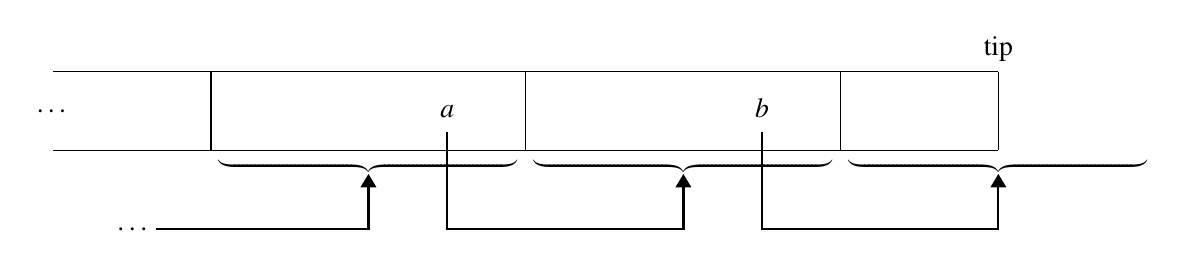
\begin{tikzpicture}
%                             /--------\
%                             |        |
%                             *        v  tip
% 1 -----+------------+------------+-----+
%        |       *    |            |     * current stake
% 0 -----+------------+------------+-----|
%   -10  -8           -4           0     2
%                |          ^
%                \----------/
\draw (-10, 0.5) node{\ldots};
\draw (-10,  0) --  (2, 0);
\draw (-10,  1) --  (2, 1);
\draw  (-8,  0) -- (-8, 1);
\draw  (-4,  0) -- (-4, 1);
\draw   (0,  0) --  (0, 1);
\draw   (2,  0) --  (2, 1) node[above]{tip};
\draw  (-6, -0.2) node {$\underbrace{\hspace{3.8cm}}$};
\draw  (-2, -0.2) node {$\underbrace{\hspace{3.8cm}}$};
\draw  ( 2, -0.2) node {$\underbrace{\hspace{3.8cm}}$};
\draw [thick, arrows={-Triangle}] (-9, -1) node[fill=white] {$\ldots$}-- (-6, -1) -- (-6, -0.3);
\draw [thick, arrows={-Triangle}] (-5, 0.5) node[fill=white] {$\mathstrut a$} -- (-5, -1) -- (-2, -1) -- (-2, -0.3);
\draw [thick, arrows={-Triangle}] (-1, 0.5) node[fill=white] {$\mathstrut b$} -- (-1, -1) -- (2, -1) -- (2, -0.3);
\end{tikzpicture}
\end{center}
%
This makes it possible to \emph{forecast} what the stake distribution (i.e.,
the ledger view) will be at various points. For example, if the chain looks like
%
\begin{center}
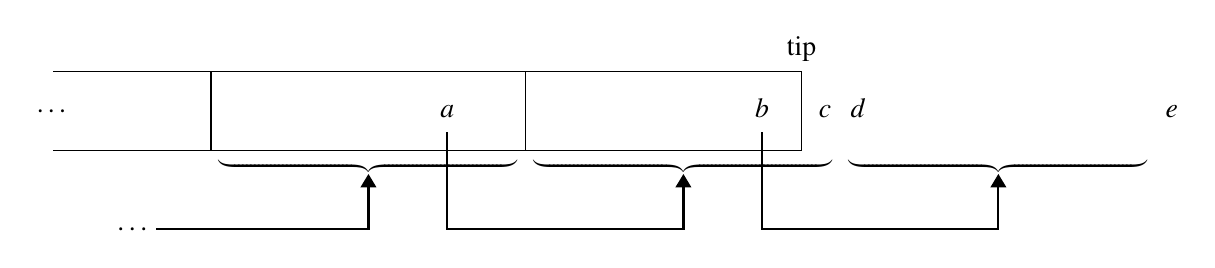
\begin{tikzpicture}
\draw (-10,    0.5) node{\ldots};
\draw (-10,    0) -- (-0.5, 0);
\draw (-10,    1) -- (-0.5, 1);
\draw  (-8,    0) -- (-8,   1);
\draw  (-4,    0) -- (-4,   1);
\draw  (-0.5,  0) -- (-0.5, 1) node[above]{tip};
\draw  (-6,   -0.2) node {$\underbrace{\hspace{3.8cm}}$};
\draw  (-2,   -0.2) node {$\underbrace{\hspace{3.8cm}}$};
\draw  ( 2,   -0.2) node {$\underbrace{\hspace{3.8cm}}$};
\draw [thick, arrows={-Triangle}] (-9, -1) node[fill=white] {$\ldots$}-- (-6, -1) -- (-6, -0.3);
\draw [thick, arrows={-Triangle}] (-5, 0.5) node[fill=white] {$\mathstrut a$} -- (-5, -1) -- (-2, -1) -- (-2, -0.3);
\draw [thick, arrows={-Triangle}] (-1, 0.5) node[fill=white] {$\mathstrut b$} -- (-1, -1) -- (2, -1) -- (2, -0.3);
\draw (0, 0.5) node[left] {$\mathstrut c$};
\draw (0, 0.5) node[right] {$\mathstrut d$};
\draw (4, 0.5) node[right] {$\mathstrut e$};
\end{tikzpicture}
\end{center}
%
then we can ``forecast'' that the stake distribution at point $c$ will be the one
established at point $a$, whereas the stake distribution at point $d$ will be the
one established at point $b$. The stake distribution at point $e$ is however not
yet known; we say that $e$ is ``out of the forecast range''.

\subsection{Code}

Since we're always forecasting what the ledger would look like \emph{if it would
be advanced to a particular slot}, the result of forecasting is always something
ticked:\footnote{An \emph{unticked} ledger view would arise from deriving the
ledger view from the \emph{current} ledger state, not taking (nor needing to
take) into account any changes that have been scheduled for later slots. The
unticked ledger view is however rarely useful; when we validate a header, any
changes that have been scheduled in the most recent ledger state for slots
before or at the slot number of the header must be applied before we validate
the header; we therefore almost exclusively work with ticked ledger views.}
%
\begin{lstlisting}
data Forecast a = Forecast {
      forecastAt  :: WithOrigin SlotNo
    , forecastFor :: SlotNo -> Except OutsideForecastRange (Ticked a)
    }
\end{lstlisting}
%
Here \lstinline!forecastAt! is the tip of the ledger in which the forecast was
constructed and \lstinline!forecastFor! is constructing the forecast for a
particular slot, possibly returning an error message of that slot is out of
range. This terminology---a forecast constructed \emph{at} a slot
and computed \emph{for} a slot---is used throughout both this technical report
as well as the consensus layer code base.

\subsection{Ledger view}
\label{forecast:ledgerview}

For the ledger view specifically, the \lstinline!LedgerSupportsProtocol!
class (\cref{ledger:api:LedgerSupportsProtocol}) requires a function
%
\begin{lstlisting}
ledgerViewForecastAt ::
     LedgerConfig blk
  -> LedgerState blk
  -> Forecast (LedgerView (BlockProtocol blk))
\end{lstlisting}
%
This function must satisfy two important properties:
%
\begin{description}
\item[Sufficient range]

When we validate headers from an upstream node, the most recent usable ledger
state we have is the ledger state at the intersection of our chain and the chain
of the upstream node. That intersection will be at most $k$ blocks back, because
that is our maximum rollback (\cref{consensus:overview:k}). Furthermore, it is
only useful to track an upstream peer if we might want to adopt their blocks,
and we only switch to their chain if it is longer than ours
(\cref{consensus:overview:chainsel}). This means that in the worst case
scenario, with the intersection $k$ blocks back, we need to be able to evaluate
$k + 1$ headers in order to adopt the alternative chain. However, the range of a
forecast is based on \emph{slots}, not blocks; since not every slot may contain
a block (\cref{time:slots-vs-blocks}), the range needs to be sufficient to
\emph{guarantee} to contain at least $k + 1$ blocks\footnote{Due to a
misalignment between the consensus requirements and the Shelley specification,
this is not the case for Shelley, where the effective maximum rollback is in
fact $k - 1$; see \cref{shelley:forecasting}).}; we will come back to this in
\cref{future:block-vs-slot}.

The network layer may have additional reasons for wanting a long forecast
range; see \cref{nonfunctional:network:headerbody}.

\item[Relation to ticking]
Forecasting is not the only way that we can get a ledger view for a particular
slot; alternatively, we can also \emph{tick} the ledger state, and then ask
for the ledger view at that ticked ledger state. These two ways should give us
the same answer:
%
\begin{equation}
\begin{array}{lllll}
\mathrm{whenever} &
\mathtt{forecastFor} \; (\mathtt{ledgerViewForecastAt}_\mathit{cfg} \; l) \; s & = & \mathtt{Right} & l' \\
\mathrm{then} & \mathtt{protocolLedgerView}_\mathit{cfg} \; (\mathtt{applyChainTick}_\mathit{cfg} \; s \; l) & = && l'
\end{array}
\end{equation}
%
In other words, whenever the ledger view for a particular slot is within the
forecast range, then ticking the ledger state to that slot and asking for the
ledger view at the tip should give the same answer. Unlike forecasting, however,
ticking has no maximum range. The reason is the following fundamental difference between these two concepts:
%
\begin{quote}
\textbf{(Forecast vs. ticking)} When we \emph{forecast} a ledger view, we are
predicting what that ledger view will be, \emph{no matter which blocks will  be
applied to the chain} between the current tip and the slot of the forecast. By
contrast, when we \emph{tick} a ledger, we are applying any time-related
changes to the ledger state in order to apply the \emph{next} block; in other
words, when we tick to a particular slot, \emph{there \emph{are} no blocks in
between the current tip and the slot we're ticking to}. Since there are no
intervening blocks, there is no uncertainty, and hence no limited range.
\end{quote}
\end{description}

\section{Queries}
\label{ledger:queries}

\section{Abandoned approach: historical states}

\chapter{Epoch Boundary Blocks}
\label{ebbs}

\section{Introduction}

Recall that when a new epoch begins, the active stake distribution in the new
epoch---that is, the stake distribution used to determine the leader schedule---
is not the stake distribution as it was at the end of the last epoch, but
rather as it was some distance back:
%
\begin{center}
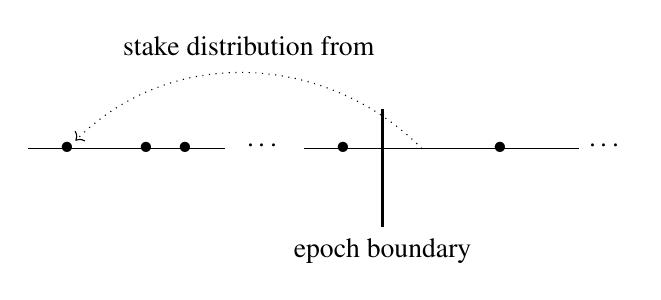
\begin{tikzpicture}
\draw
     (0   , 0)
  -- (0.5 , 0) node{$\bullet$}
  -- (1.5 , 0) node{$\bullet$}
  -- (2   , 0) node{$\bullet$}
  -- (2.5 , 0);
\node at (3,0) {$\cdots$};
\draw
     (3.5 , 0)
  -- (4   , 0) node{$\bullet$}
  -- (6   , 0) node{$\bullet$}
  -- (7   , 0) node[right]{$\cdots$};
\draw [very thick] (4.5,0.5) -- (4.5,-1) node[below] {epoch boundary};
\draw [->, dotted] (5,0) to [out=135,in=45] (0.6,0.1);
\path (5,0) -- (0.6,0.1) node[pos=0.5,above=1] {stake distribution from};
\end{tikzpicture}
\end{center}
%
This means that blocks cannot influence the active stake distribution until
some time in the future. That is important, because when a malicious node
forks off from the honest chain, the leadership schedule near the intersection
point cannot be influenced by the attacker, allowing us to compare chain
density and choose the honest chain (which will be denser because of the
assumed honest majority); see \cref{genesis} for an in-depth discussion.

In the literature, the term ``epoch boundary block'' (or EBB for short) normally
simply refers to the last block in any given epoch (for example,
see~\cite{buterin2020combining}). It might therefore be a bit surprising to find
the term in this report since the final block in an epoch is not of special
interest in the Ouroboros family of consensus protocols. However, in the first
implementation of the Byron ledger (using the original Ouroboros protocol
\cite{cryptoeprint:2016:889}, which we now refer to as ``Ouroboros Classic''), a
decision was made to include the leadership schedule for each new epoch as an
explicit block on the blockchain; the term EBB was used to refer to this special
kind of block:\footnote{It is not entirely clear if an EBB should be regarded as
the final block in an epoch, or as the first block in the next epoch. The name
would suggest that the former interpretation is more appropriate; as it turns
out, however, the very first epoch on the chain \emph{starts} with an EBB,
recording the leadership schedule derived from the genesis block. We will
therefore regard the EBB as starting an epoch, rather than ending one.}
%
\begin{center}
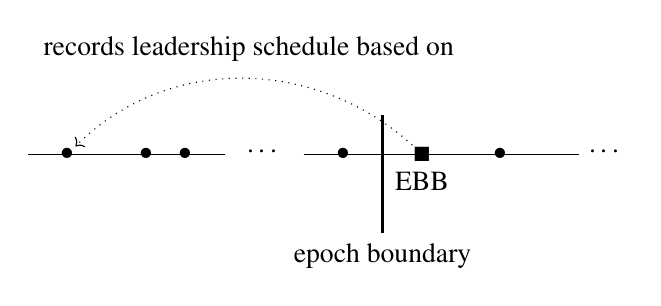
\begin{tikzpicture}
\draw
     (0   , 0)
  -- (0.5 , 0) node{$\bullet$}
  -- (1.5 , 0) node{$\bullet$}
  -- (2   , 0) node{$\bullet$}
  -- (2.5 , 0);
\node at (3,0) {$\cdots$};
\draw
     (3.5 , 0)
  -- (4   , 0) node{$\bullet$}
  -- (6   , 0) node{$\bullet$}
  -- (7   , 0) node[right]{$\cdots$};
\draw [very thick] (4.5,0.5) -- (4.5,-1) node[below] {epoch boundary};
\draw [->, dotted] (5,0) to [out=135,in=45] (0.6,0.1);
\path (5,0) -- (0.6,0.1) node[pos=0.5,above=1] {records leadership schedule based on};
\node at (5,0) {$\blacksquare$};
\node [below=0.1] at (5,0) {EBB};
\end{tikzpicture}
\end{center}

Having the leadership schedule explicitly recorded on-chain turns out not to
be particularly useful, however, and the code was modified not to produce EBBs
anymore even before we switched from Byron to Shelley (as part of the OBFT hard
fork, see \cref{overview:history}); these days, the contents of the existing
EBBs on the chain are entirely ignored. Unfortunately, we cannot forget about
EBBs altogether because---since they are an actual block on the
blockchain---they affect the chain of block hashes: the first ``real'' block in
each epoch points to the EBB as its predecessor, which then in turns points to
the final block in the previous epoch.

So far, none of this is particularly problematic to the consensus layer. Having
multiple types of blocks in a ledger presents some challenges for serialisation
(\cref{serialisation:storage:nested-contents}), but does not otherwise affect
consensus much: after all, blocks are interpreted by the ledger layer, not by
the consensus layer. Unfortunately, however, the design of the Byron EBBs has
odd quirk: an EBB has the same block number as its \emph{predecessor}, and the
same slot number as its \emph{successor}:
%
\begin{center}
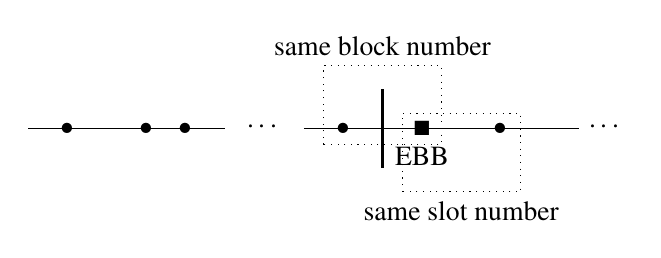
\begin{tikzpicture}
\draw
     (0   , 0)
  -- (0.5 , 0) node{$\bullet$}
  -- (1.5 , 0) node{$\bullet$}
  -- (2   , 0) node{$\bullet$}
  -- (2.5 , 0);
\node at (3,0) {$\cdots$};
\draw
     (3.5 , 0)
  -- (4   , 0) node{$\bullet$}
  -- (6   , 0) node{$\bullet$}
  -- (7   , 0) node[right]{$\cdots$};
\draw [very thick] (4.5,0.5) -- (4.5,-0.5);
\node at (5,0) {$\blacksquare$};
\node [below=0.1] at (5,0) {EBB};
%
\draw [dotted]
     (3.75, -0.2)
  -- ++(0, 1)
  -- ++(1.5, 0) node[pos=0.5,above] {same block number}
  -- ++(0, -1)
  -- cycle;
\draw [dotted]
     (4.75, -0.8)
  -- ++(0, 1)
  -- ++(1.5, 0)
  -- ++(0, -1)
  -- cycle  node[pos=0.5,below] {same slot number};
\end{tikzpicture}
\end{center}
%
This turns out to be a huge headache. When we started the rewrite, I think we
underestimated quite how many parts of the system would be affected by the
possibility of having multiple blocks with the same block number and
multiple blocks with the same slot number on a single chain. Some examples
include:

\begin{itemize}
\item \label{ebb-chain-selection}
For chain selection protocols based on chain length, two chains may end in
blocks with the same block number, yet not have equal length.

\item When we validate block headers that contain explicit block numbers, we
cannot insist that those block numbers are monotonically increasing, instead
having to add a special case for EBBs.

\item TODO: Many, many others
\end{itemize}

In hindisght, we should have tried harder to eliminate EBBs from the get-go. In
this chapter, we will discuss two options for modifying the existing design to
reduce the impact of EBBs (\cref{ebbs:logical}), or indeed eliminate them
altogether (\cref{ebbs:elimination}).

\section{Logical slot/block numbers}
\label{ebbs:logical}

\section{Eliminating EBBs altogether}
\label{ebbs:elimination}









% For the Ouroboros family of consensus
% protocols, the last block in an epoch is not of special interest, so it
% might be surprising to see the term EBB in this report.
%
% When a new epoch
% begins---that is, at an epoch boundary---the active stake distribution shifts,
% but it is not based on the final block in the previous epoch, but instead on
% the ledger state as it was quite a bit earlier. As a consequence, blocks cannot
% have an effect on the leadership schedule until they are a certain depth into
% the chain. This is important, because it means that if there is a fork in the
% chain, the leadership schedule after the intersection point will be determined
% by the common prefix of both chains.


%
%
% section 3 (The Ouroboros Protocol)
%
% Stage 1: "There is an initial stake distribution which is hardcoded into the genesis block"


% Discuss that although EBBs are a Byron concern, their presence has far reaching
% consequences on the consensus later. In hindsight, we should have tried harder
% to not deal with them at all from the beginning; we did not anticipate quite how
% bad the situation would be. We now have a plan for getting rid of them
% (\cref{decontamination-plan}) but it will be a fairly long term thing and it
% might not happen at all, depending on quite how much time is available for
% removing tech debt.
%
%
% \section{Introduction}
%
% \section{Consequences}
%
% \subsection{Chain selection}
% \label{ebb-chain-selection}
%
% \section{Elimination}
% \label{decontamination-plan}


\part{Storage Layer}

\chapter{Overview}
\label{hfc}

\section{Introduction}
\label{hfc:intro}

\todo{} We should discuss terminology here: what we mean by a hard fork,
and how that is different from how the word is usually used.

We should mention that era transitions happen at epoch boundaries only.

Mention that we had to adjust the consensus layer in some ways:

\begin{itemize}
\item Simplified chain selection (tip only; \cref{chain-selection:overview})
\item Remove the assumption slot/time conversion is always possible (\cref{time})
\end{itemize}

\newcommand{\chunkNumber}[1]{\ensuremath{\mathsf{chunkNumber}(#1)}}
\newcommand{\relativeSlot}[2]{\ensuremath{\mathsf{relativeSlot}(#1, #2)}}

\chapter{Immutable Database}
\label{immutable}

The Immutable DB is tasked with storing the blocks that are part of the
\emph{immutable} part of the chain. Because of the nature of this task, the
requirements and \emph{non-requirements} of this component are fairly specific:

\begin{itemize}
\item \textbf{Append-only}: as it represents the immutable chain, blocks will
  only be appended in the same order as they are ordered in the chain. Blocks
  will never be \emph{modified} or \emph{deleted}.
\item \textbf{Reading}: the database should be able to return the block or
  header stored at a given \emph{point} (combination of slot number and hash)
  efficiently.\todo{define point somewhere?}
\item \textbf{Efficient streaming}: when serving blocks or headers to other
  nodes, we need to be able to stream ranges of \emph{consecutive} blocks or
  headers efficiently. As described in \cref{serialisation:network:serialised},
  it should be possible to stream \emph{raw} blocks and headers, without
  serialising them.
\item \textbf{Recoverability}: it must be possible to validate the blocks stored
  in the database. When a block in the database is corrupt or missing, it is
  sufficient to truncate the database, representing an immutable chain, to the
  last valid block before the corrupt or missing block. The truncated blocks can
  simply be downloaded again. It is therefore not necessary to be able recover
  the full database when blocks are missing.
\end{itemize}

While we touched upon some of the non-requirements already above, it is useful
to highlight the following non-requirements.

\begin{itemize}
\item \textbf{Queries}: besides looking up a single block by its point and
  streaming ranges of consecutive blocks, the database does have to be able to
  answer queries about blocks. No searching or filtering is needed.
\item \textbf{Durability}: the system does not require the durability guarantee
  that traditional database systems provide (the D in ACID). If the system
  crashes right after appending a block, it is acceptable that the block in
  question is truncated when recovering the database. Because of the overlap
  with the Volatile DB\todo{link}, such a truncation is likely to even go
  unnoticed. In the worst case, the truncated blocks can simply be downloaded
  again.
\end{itemize}

Because of the specific requirements and non-requirements listed above, we
decided to write our own implementation, the \lstinline!ImmutableDB!, instead of
using an existing off-the-shelf database system. Traditional database systems
provide guarantees that are not needed and, conversely, do not take advantage of
the requirements to optimise certain operations. For example, there is no need
for a journal or flushing (\lstinline!fsync!) the buffers after each write
because of our unique durability and recoverability (non-)requirements.

\section{API}
\label{immutable:api}

Before we describe the implementation of the Immutable DB, we first describe its
functionality. The Immutable DB has the following API:

\begin{lstlisting}
data ImmutableDB m blk = ImmutableDB {
      closeDB :: m ()

    , getTip :: STM m (WithOrigin (Tip blk))

    , appendBlock :: blk -> m ()

    , getBlockComponent ::
           forall b.
           BlockComponent blk b
        -> RealPoint blk
        -> m (Either (MissingBlock blk) b)

    , stream ::
           forall b.
           ResourceRegistry m
        -> BlockComponent blk b
        -> StreamFrom blk
        -> StreamTo   blk
        -> m (Either (MissingBlock blk) (Iterator m blk b))
    }
\end{lstlisting}

The database is parameterised over the block type \lstinline!blk! and the monad
\lstinline!m!, like most of the consensus layer.\todo{mention io-sim}
\todo{TODO} Mention our use of records for components?

The \lstinline!closeDB! operation closes the database, allowing all opened
resources, including open file handles, to be released. This is typically only
used when shutting down the entire system. Calling any other operation on an
already-closed database should result in an exception.

The \lstinline!getTip! operation returns the current tip of the Immutable DB.
The \lstinline!Tip! type contains information about the block at the tip like
the slot number, the block number, the hash, etc. The \lstinline!WithOrigin!
type is isomorphic to \lstinline!Maybe! and is used to account for the
possibility of an empty database, i.e., when the tip is at the ``origin'' of the
chain. This operation is an \lstinline!STM! operation, which allows it to be
combined with other \lstinline!STM! operations in a single transaction, to
obtain a consistent view on them. This also implies that no IO or disk access is
needed to obtain the current tip.

The \lstinline!appendBlock! operation appends a block to the Immutable DB. As
slot numbers increase monotonically in the blockchain, the block's slot must be
greater than the current tip's slot (or equal when the tip points at an EBB, see
\cref{ebbs}). It is not required that each slot is filled,\todo{link?} so there
can certainly be gaps in the slot numbers.

The \lstinline!getBlockComponent! operation allows reading one or more
components of the block in the database at the given point. We discuss what
block components are in \cref{immutable:api:block-component}. The
\lstinline!RealPoint! type represents a point that can only refer to a block,
not to genesis (the empty chain), which the larger \lstinline!Point! type
allows. As the given point might not be in the Immutable DB, this operation can
also return a \lstinline!MissingBlock! error instead of the requested block
component.

The \lstinline!stream! operation returns an iterator to efficiently stream the
blocks between the two given bounds. The bounds are defined as such:
\begin{lstlisting}
data StreamFrom blk =
    StreamFromInclusive !(RealPoint blk)
  | StreamFromExclusive !(Point     blk)

newtype StreamTo blk =
    StreamToInclusive (RealPoint blk)
\end{lstlisting}
Lower bounds can be either inclusive or exclusive, but exclusive upper bounds
were omitted because they were not needed in practice. An inclusive bound must
refer to a block, not genesis, hence the use of \lstinline!RealPoint!. The
exclusive lower bound \emph{can} refer to genesis, hence the use of
\lstinline!Point!, in particular to begin streaming from the start of the chain.
As one or both of the bounds might not be in the Immutable DB, this operation
can return a \lstinline!MissingBlock! error. We discuss what block components
are in \cref{immutable:api:block-component}. The \lstinline!ResourceRegistry!
will be used to allocate all the resources the iterator opens during its
lifetime, e.g., file handles. By closing the registry in case of an exception
(using \lstinline!bracket!), all open resources are released and nothing is
leaked.\todo{link} More discussion about iterators follows in
\cref{immutable:api:iterators}.

\subsection{Block Component}
\label{immutable:api:block-component}

\todo{TODO} move to ChainDB?

Besides reading or streaming blocks from the Immutable DB, it must be possible
to read or stream headers, raw blocks (see
\cref{serialisation:network:serialised}), but in some cases also \emph{nested
contexts} (see \cref{serialisation:storage:nested-contents}) or even block
sizes. Adding an operation to the API for each of these would result in too much
duplication. We handle this with the \lstinline!BlockComponent! abstraction:
when reading or streaming, one can choose which \emph{components} of a block
should be returned, e.g., the block itself, the header of the block, the size of
the block, the raw block, the raw header, etc. We model this with the following
GADT:

\begin{lstlisting}
data BlockComponent blk a where
  GetVerifiedBlock :: BlockComponent blk blk
  GetBlock         :: BlockComponent blk blk
  GetRawBlock      :: BlockComponent blk ByteString
  GetHeader        :: BlockComponent blk (Header blk)
  GetRawHeader     :: BlockComponent blk ByteString
  GetHash          :: BlockComponent blk (HeaderHash blk)
  GetSlot          :: BlockComponent blk SlotNo
  GetIsEBB         :: BlockComponent blk IsEBB
  GetBlockSize     :: BlockComponent blk Word32
  GetHeaderSize    :: BlockComponent blk Word16
  GetNestedCtxt    :: BlockComponent blk (SomeSecond (NestedCtxt Header) blk)
  ..
\end{lstlisting}
The \lstinline!a! type index determines the type of the block component.
Additionally, we have \lstinline!Functor! and \lstinline!Applicative! instances.
The latter allows combining multiple \lstinline!BlockComponent!s into one. This
can be considered a small DSL for querying components of a block.

\subsection{Iterators}
\label{immutable:api:iterators}

The following API can be used to interact with an iterator:

\begin{lstlisting}
data Iterator m blk b = Iterator {
      iteratorNext    :: m (IteratorResult b)
    , iteratorHasNext :: STM m (Maybe (RealPoint blk))
    , iteratorClose   :: m ()
    }

data IteratorResult b =
    IteratorExhausted
  | IteratorResult b
\end{lstlisting}

The \lstinline!iteratorNext! operation returns the current
\lstinline!IteratorResult! and advances the iterator to the next block in the
stream. When the iterator has reached its upper bound, it is exhausted. Remember
that the \lstinline!b! type argument corresponds to the requested block
component.

The \lstinline!iteratorHasNext! operation returns the point corresponding to the
block the next call to \lstinline!iteratorNext! will return. When exhausted,
\lstinline!Nothing! is returned.

As an open iterator can hold onto resources, e.g., open file handles, it should
be explicitly closed using the \lstinline!iteratorClose! operation. Interacting
with a closed iterator should result in an exception, except for calling
\lstinline!iteratorClose!, which is idempotent.

\section{Implementation}
\label{immutable:implementation}

We will now give a high-level overview of our custom implementation of the
Immutable DB that satisfies the requirements and the API.

\begin{itemize}
\item We store blocks sequentially in a file, called a \emph{chunk file}. We
  append each raw block, without any extra information before or after it, to
  the chunk file. This will facilitate efficient binary streaming of blocks. In
  principle, it is a matter of copying bytes from one buffer to another, without
  any additional processing needed.

\item Every $x$ \emph{slots}, where $x$ is the configurable chunk size, we start
  a new chunk file to avoid storing all blocks in a single file.

\item To facilitate looking up a block by a point, which consists of the hash
  and the slot number, we ``index'' our database by slot numbers. One can then
  look up the block in the given slot and compare its hash against the point's
  hash. No searching will be needed.

  Blocks are stored sequentially in chunk files, but slot numbers do \emph{not}
  increase one-by-one; they are \emph{sparse}. This means we need a mapping from
  the slot number to the offset and size of the block in the chunk file. We
  store this mapping in the on-disk \emph{primary index}, one per chunk file,
  which we discuss in more detail in \cref{immutable:implementation:indices}.

\item As mentioned above, when looking up a block by a point, we will compare
  the hash of the block at the point's slot in the Immutable DB with the point's
  hash. We should be able to do this without first having to read and
  deserialise the entire block in order to know its hash.

  Moreover, it should be possible to read just the header of the block without
  first having to read the entire block. As described in
  \cref{serialisation:storage:nested-contents}, we can do this if have access to
  the header offset, header size, and nested context of the block.

  For these reasons, we store the aforementioned extra information, which should
  be available without having to read and deserialise the entire block,
  separately in the on-disk \emph{secondary index}, one per chunk file
  (\cref{immutable:implementation:indices}).

\item All the information stored in the primary and secondary indices can be
  recovered from the blocks in the chunk files. This is described in
  \cref{immutable:implementation:recovery}.

\item Whenever a file-system operation fails, or a file is missing or corrupted,
  we shut down the Immutable DB and consequently the whole system. When this
  happens, either the system's file system is no longer reliable (e.g., disk
  corruption), manual intervention (e.g., disk is full) is required, or there is
  a bug in the system. In all cases, there is no point in trying to continue
  operating. We shut down the system and flag the shutdown as \emph{dirty},
  triggering a full validation on the next start-up, see
  \cref{immutable:implementation:recovery}.

  Not all forms of disk corruption can easily be detected. For example, when
  some bytes in a block stored in a chunk file have been flipped on disk, this
  can easily go unnoticed. Deserialising the block might fail if the
  serialisation format is no longer valid, but the bitflip could also happen in,
  e.g., the amount of a transaction, which will not be detected by the
  deserialiser. In fact, the majority of blocks read will not even be
  deserialised, as blocks served to other nodes are read and sent in their raw,
  still serialised format. However, sending a corrupted block must be avoided,
  as nodes receiving it will consider it invalid and can blacklist us, mistaking
  us for an adversary.

  To detect such forms of silent corruption, we store CRC32 checksums in the
  secondary index (\cref{immutable:implementation:indices}) which we verify when
  reading the block, which we can do even when not deserialising the block. Note
  that we could use the block's own hash for this purpose,\footnote{To be
  precise: we would have to check the block body against the body hash stored in
  the header, and verify the signature of the header.} but because computing
  such a cryptographic hash is much more expensive, we opted for a separate
  CRC32 checksum, which is much more efficient to compute and designed for
  exactly this purpose.

\item We store the state of the current chunk, including its indices, in memory.
  We store this state, a pure data type, in a \lstinline!StrictMVar!. Besides
  avoiding space leaks by forcing its contents to WHNF, this
  \lstinline!StrictMVar! type has another useful ability that its standard
  non-strict variant is lacks: while it is locked when being modified, the
  previous, \emph{stale} value can still be read.

  This is convenient for the Immutable DB: we can support multiple concurrent
  reads even when at most one append operation is in progress, as it is safe to
  read a block based on the stale state because data will only be appended, not
  modified.

  To append a block to the Immutable DB, we lock the state to avoid concurrent
  append operations. We append the block to the chunk file, and append the
  necessary information to the primary and secondary indices. We unlock the
  state, updated with the information about the newly appended block.

\item We \emph{do not flush} any writes to disk, as discussed in the
  introduction of this chapter. This makes appending a block quite cheap: the
  serialised block is copied to an OS buffer, which is then asynchronously
  flushed in the background.

\item To avoid repeatedly reading and deserialising the same primary and
  secondary indices of older chunks, we cache them in a LRU-cache that is
  bounded in size.

\item To open an iterator, we check its bounds using the (cached) indices. The
  bounds are valid when both correspond to blocks present in the Immutable DB.
  Next, a file handle is opened for the chunk file containing the first block to
  stream. The same chunk file's indices are read (from the cache) and the
  iterator will maintain a list of secondary index entries, one for each block
  to stream from the chunk file. By having this list of entries in memory, the
  indices will not have to be accessed for each streamed block.

  When a block component is requested from the iterator, it is read from the
  chunk file and/or extracted from the corresponding in-memory entry.
  Afterwards, the entry is dropped from the in-memory list so that the next
  entry is ready to be read. When the list of entries is exhausted without
  reaching the end bound, we move on to the next chunk file. This process
  repeats until the end bound is reached.
\end{itemize}

\subsection{Chunk layout}
\label{immutable:implementation:chunk-layout}

Each block in the block chain has a unique slot number (except for EBBs, which
we discuss below). Slot numbers increase in the blockchain, but not all slots
have to be filled. For example, in the Byron era (using the Permissive BFT
consensus algorithm), nearly every slot will be filled, but in the Shelley era
(using the Praos consensus algorithm), on average only one in twenty slots will
be filled.

As mentioned above, we want to group blocks into chunk files. Because we need to
be able to look up blocks in the Immutable DB based on their slot number, we
group blocks into chunk files based on their slot numbers so that the chunk file
containing a block can be determined by looking at the slot number of the block.

Internally, we translate \emph{absolute} slot numbers into \emph{chunk numbers}
and \emph{relative slot numbers} (relative w.r.t.\ the chunk). As EBBs
(\cref{ebbs}) have the same slot number as their successor, this translation is
not injective. To restore injectivity, we include ``whether the block is an EBB
or not'' as an input to the translation.

\todo{TODO} how should this be formatted?

\begin{definition}[Chunk number]
  Let $s$ be the absolute slot number of a block. Using a chunk size of
  $\mathit{sz}$:

  \[
  \chunkNumber{s} = \lfloor s / \mathit{sz} \rfloor
  \]
  Naturally, chunks are zero-indexed.

\end{definition}

\begin{definition}[Relative slot number]
  Let $s$ be the absolute slot number of a block. Using a chunk size of
  $\mathit{sz}$:

  \[
  \relativeSlot{s}{\mathit{isEBB}} =
  \begin{cases}
    0                         & \text{if}\,\mathit{isEBB} \\
    (s \bmod \mathit{sz}) + 1 & \text{otherwise}
  \end{cases}
  \]
  We reserve the very first relative slot for an EBB, hence the need to make
  room for it by incrementing by one in the non-EBB case.
\end{definition}

In the example below, we show a chunk with chunk number 1 using a chunk size of
100:

\begin{center}
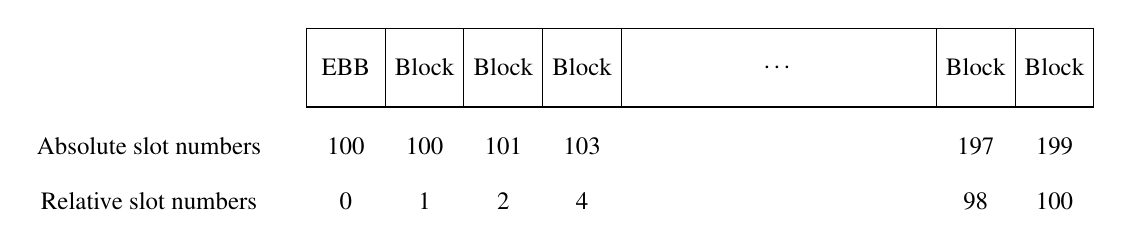
\begin{tikzpicture}
\draw (0, 0) -- (10, 0);
\draw (0, 1) -- (10, 1);

\draw ( 0, 0) -- ( 0, 1);
\draw ( 1, 0) -- ( 1, 1);
\draw ( 2, 0) -- ( 2, 1);
\draw ( 3, 0) -- ( 3, 1);
\draw ( 4, 0) -- ( 4, 1);
\draw ( 8, 0) -- ( 8, 1);
\draw ( 9, 0) -- ( 9, 1);
\draw (10, 0) -- (10, 1);

\draw (0.5, 0.5) node {\small EBB};
\draw (1.5, 0.5) node {\small Block};
\draw (2.5, 0.5) node {\small Block};
\draw (3.5, 0.5) node {\small Block};
\draw (6.0, 0.5) node {\small \ldots};
\draw (8.5, 0.5) node {\small Block};
\draw (9.5, 0.5) node {\small Block};

\draw (-2.0, -0.5) node {\small Absolute slot numbers};
\draw ( 0.5, -0.5) node {\small 100};
\draw ( 1.5, -0.5) node {\small 100};
\draw ( 2.5, -0.5) node {\small 101};
\draw ( 3.5, -0.5) node {\small 103};
\draw ( 8.5, -0.5) node {\small 197};
\draw ( 9.5, -0.5) node {\small 199};

\draw (-2.0, -1.2) node {\small Relative slot numbers};
\draw ( 0.5, -1.2) node {\small 0};
\draw ( 1.5, -1.2) node {\small 1};
\draw ( 2.5, -1.2) node {\small 2};
\draw ( 3.5, -1.2) node {\small 4};
\draw ( 8.5, -1.2) node {\small 98};
\draw ( 9.5, -1.2) node {\small 100};
\end{tikzpicture}
\end{center}
Note that some slots are empty, e.g., 102 and 198 are missing. The first and
lasts slots can be empty too. In practice, it will never be the case that an
entire chunk is empty, but the implementation allows for it.

If we were to pick a chunk size of 1 and store each block in its own file, we
would need millions of files, as there are millions of blocks. When serving
blocks to peer, we would constantly open and close individual block files, which
is very inefficient.

If we pick a very large or even unbounded chunk size, the resulting chunk file
would be several gigabytes in size and keep growing. This would make the
recovery process (\cref{immutable:implementation:recovery}) more complicated and
potentially much slower, as more data might have to be read and
validated.\todo{Other arguments?} Moreover, our current approach of caching
indices per chunk would have to be revised.

In practice, a chunk size of \num{21600} is used, which matches the \emph{epoch
size} of Byron. It is no coincidence that there is (at most) one EBB at the
start of each Byron epoch, fitting nicely in the first relative slot that we
reserve for it. Originally, the Immutable DB called these chunk files
\emph{epoch files}. With the advent of Shelley, which has a different epoch size
than Byron, we decoupled the two and introduced the name ``chunk''.

\paragraph{Dynamic chunk size}

The \emph{chunking} scheme was designed with the possibility of a non-uniform
chunk size in mind. Originally, the goal was to make the chunk size configurable
such that the number of slots per chunk could change after a certain slot.
Similarly, the reserving an extra slot for an EBB would be optional and could
stop after a certain slot, i.e., when the production of EBBs stopped. The
reasoning behind this was to allow the chunk size to change near the transition
from Byron to Shelley. As the slot density goes down by a factor of twenty when
transitioning to Shelley, the number of blocks per chunk file and, consequently,
the chunk size would go down by the same factor, leading to too many, smaller
chunk files. The intention was to configure the chunk size to increase by the
same factor at the start of the Shelley era.

The transition to another era, e.g., Shelley, is dynamic: the slot at which it
happens is determined by on-chain voting and is not certain up to a number of
hours in advance. Making the mapping from slot number to chunk and relative slot
number rely on the actual slot at which the transition happened would complicate
things significantly. It would make the mapping depend on the ledger state,
which determines the current era. This would make an unwanted coupling between
the Immutable DB, storing \emph{blocks}, to the ledger state obtained by
applying these blocks. A reasonable compromise would be to hard-code the change
in chunk size to the estimated transition slot. When the estimate is incorrect,
only a few Byron chunks would contain more blocks than intended or only a few
Shelley chunks would contain fewer blocks than intended.

Unfortunately, due to lack of time, dynamic chunk sizes were not implemented in
time for the transition to Shelley. This means the same chunk size is being used
for the \emph{entire chain}, resulting in fewer blocks per Shelley chunk file
than ideal, and, consequently, more chunk files than ideal.

\paragraph{Indexing by block number}

The problem of too small, too many chunk files described in the paragraph above
is caused by the fact that slot numbers can be sparse and do not have to be
consecutive. \emph{Block numbers} do not have the same problem: they are
consecutive and thus dense, regardless the era of the blockchain. If instead of
indexing the Immutable DB by slot numbers, we indexed it by \emph{block
numbers}, we would not have the problem. Unfortunately, the point type, which is
used throughout the network layer and the consensus layer to identify and look
up blocks, consists of a hash and \emph{slot number}, not a block number.

Either we would have to maintain another index from slot number to block number,
which would require its own chunking scheme based on slot numbers or just one
big file, which has its own downsides. Or, points should be based on block
numbers instead of slot numbers. As points are omnipresent, this change is very
far-reaching. The latter approach carries our preference, but is currently out
of the question. The former is more localised, but the complexity and risks
involved in migrating deployed on-disk databases to the new format do not
outweigh the uncertain benefits.

\subsection{Indices}
\label{immutable:implementation:indices}

As mentioned before, we have on-disk indices for the chunk files for two
purposes:
\begin{enumerate}
\item To map the sparse slot numbers to the blocks that are densely stored in
  the chunk files.
\item To store the information about a block that should be available without
  having to read and deserialise the actual block, e.g., the header offset, the
  header size, the CRC32 checksum, etc.
\end{enumerate}
We use a separate index for each task: the \emph{primary index} for the first
task and the \emph{secondary index} for the second task. Each chunk file has a
corresponding primary index file and secondary index file. Because of a
dependency of the primary index on the secondary index, we first discuss the
latter.

\paragraph{Secondary index}

In the secondary index, we store the information about a block that is needed
before or without having to read and deserialise the block. The secondary index
is an append-only file, like the chunk file, and contains a \emph{secondary
index entry} for each block. For simplicity and robustness, a secondary index
merely contains a series of densely stored secondary index entries with no extra
information between, before, or after them. This avoids needing to initialise or
finalise such a file, which also makes the recovery process simpler
(\cref{immutable:implementation:recovery}). A secondary index entry consists of
the following fields:

\begin{center}
\begin{tabular}{l r}
  field & size [bytes] \\
  \hline
  block offset  & 8 \\
  header offset & 2 \\
  header size   & 2 \\
  checksum      & 4 \\
  header hash   & X \\
  block or EBB  & 8 \\
\end{tabular}
\end{center}

\begin{itemize}
\item The block offset is used to determine at which offset in the corresponding
  chunk file the raw block can be read.

  As blocks are variable-sized, the size of the block also needs to be known in
  order to read it. Instead of spending another 8 bytes to store the block size
  as an additional field, we read the block offset of the \emph{next entry} in
  the secondary index, which corresponds to the block after it. The block size
  can then be computed by subtracting the latter's block offset from the
  former's.

  In case the block is the final block in the chunk file, there is no next
  entry. Instead, the final block's size can be derived from the chunk file's
  size. When reading the final block $B_n$ of the current chunk file, it is
  important to obtain the chunk file size at the right time, before any more
  blocks ($B_{n+1}, B_{n+2}, \ldots$) are appended to the same file, increasing the
  chunk file size. Otherwise, we risk reading the bytes corresponding to not
  just the previously final block $B_n$, but also $B_{n+1}, B_{n+2},
  \ldots$\footnote{In hindsight, storing the block size as a separate field would
  have simplified the implementation.}

  The reasoning behind using 8 bytes for the block offset is the following. The
  maximum block header and block body sizes permitted by the blockchain itself
  are dynamic parameters that can change through on-chain voting. At the time of
  writing, the maximum header size is 1100 bytes and the maximum body size is
  \num{65536} bytes. By multiplying this theoretical maximum block size of
  $\num{1100} + \num{65536} = \num{66636}$ bytes by the chunk size used in
  practice, i.e., \num{21600}, assuming a maximal density of 1.0 in the Byron
  era, we get \num{1439337600} as the maximal file size for a chunk file. An
  offset into a file of that size fits tightly in 4 bytes, but this would not
  support any future maximum block size increases, hence the decision to use 8
  bytes.

\item The header offset and header size are needed to extract the header from a
  block without first having to read and deserialise the entire block, as
  discussed in \cref{serialisation:storage:nested-contents}. These are stored
  per block, as the header size can differ from block to block. The nested
  context is reconstructed by reading bytes from the start of the block, as
  explained in our discussion of the \lstinline!ReconstructNestedCtxt! class in
  \cref{serialisation:storage:nested-contents}.

  Using 2 bytes for the header offset and header size is enough when taking the
  following into account: (so far all types of) blocks start with their header,
  the current maximum header size is \num{1100} bytes, and the header offset is
  relative to the start of the block.

\item As discussed before, to detect silent corruption of blocks, we store a CRC
  checksum of each block, against which the block is verified after reading it.
  This verification can be done without deserialising the block.

  Note that we do not store a checksum of the raw header, which means we do not
  check for silent corruption when streaming headers.\todo{Maybe we should?}

\item The header hash is used for lookups and bounds checking, i.e., to check
  whether the given point's hash matches the hash of the block as the same slot
  in the Immutable DB. By storing it separately, we do not have to read and
  compute the hash of the block's header just to check whether it has the right
  hash.

  The header hash field's size depends on the concrete instantiation of the
  \lstinline!HeaderHash blk! type family. In practice, a 32-byte hash is used.

\item The ``block or EBB'' field is represented in memory as follows:

  \begin{lstlisting}
  data BlockOrEBB =
      Block !SlotNo
    | EBB   !EpochNo
  \end{lstlisting}

  The former constructor represents a regular block with an absolute slot number
  and the latter an EBB (\cref{ebbs}) with an epoch number (since there is only
  a single EBB per epoch). The main reason this field is part of the secondary
  index entry is to implement the \lstinline!iteratorHasNext! method of the
  iterator API (see \cref{immutable:api:iterators}) without having to read the
  next block from disk, as the iterator will keep these secondary index entries
  in memory.

  Both the \lstinline!SlotNo! and \lstinline!EpochNo! types are newtypes around
  a \lstinline!Word64!, hence the 8 on-disk bytes. We omit the tag
  distinguishing between the two constructors in the serialisation because in
  nearly all cases, this information has already been retrieved from the primary
  index, i.e., whether the first filled slot in a chunk is an EBB or
  not.\footnote{In hindsight, having the tag in the serialisation would have
  simplified the implementation.}

\item Because of the fixed size of each field, it was originally decided to
  (de)serialise the corresponding data type using the \lstinline!Binary! class.
  Using CBOR would be more flexible to future changes. This would make the
  encoding variable-sized, which is not necessarily an issue, which will become
  clear in our description of the primary index.

\end{itemize}

\paragraph{Primary index}

The primary index maps the sparse slot numbers to the secondary index entries of
the corresponding blocks in the dense secondary index. As discussed above, the
secondary index entry of a block tells us the offset in the chunk file of the
corresponding block.

The format of the primary index is as follows. The primary index start with a
byte indicating its version number. Next, for each slot, empty or not, we store
the offset at which its secondary index entry starts in the secondary index.
This same offset will correspond to the \emph{end} of the previous secondary
index entry. When a slot is empty, its offset will be the same as the offset of
the slot before it, indicating that the corresponding secondary index entry is
empty.

When appending a new block, we append the previous offset as many times as the
number of slots that was skipped, indicating that they are empty. Next, we
append the offset after the newly appended secondary index entry corresponding
to the new block.

We use a fixed size of 4 bytes to store each offset. As this is an offset in the
secondary index, it should be at least large enough to address the maximal size
of a secondary index file. We can compute this by multiplying the used chunk
size by the size of a secondary index entry: $\num{21600} * (8 + 2 + 2 + 4 + 32
+ 8) = \num{1209600}$, which requires more than 2 bytes to address.

To look up the secondary index entry for a certain slot, we compute the
corresponding chunk number and relative slot number using $\mathsf{chunkNumber}$
and $\mathsf{relativeSlot}$ (we discuss how we deal with EBBs later). Because we
use a fixed size for each offset, based on the relative slot number, we can
compute exactly at which bytes should be read at which offset in the primary
index, i.e., the 4 + 4 bytes corresponding to the offset at the relative slot
and the offset after it. When both offsets are equal, the slot is empty. When
not equal, we now know which bytes to read from the secondary index to obtain
the secondary index entry corresponding to the block in question.

However, as mentioned in \cref{immutable:implementation}, we maintain a cache of
primary indices, which means that they are always read from disk in their
entirety. After a cache hit, looking up a relative slot in the cached primary
index corresponds to a constant-time lookup in a vector.

We illustrate this format with an example primary index below, which matches the
chunk out of the example from \cref{immutable:implementation:chunk-layout}. The
offsets correspond to the blocks on the line below them, where $\emptyset$ indicates an
empty slot. We assume a fixed size of 10 bytes for each secondary index entry.
The offset $X$ corresponds the final size of the secondary index.

\begin{center}
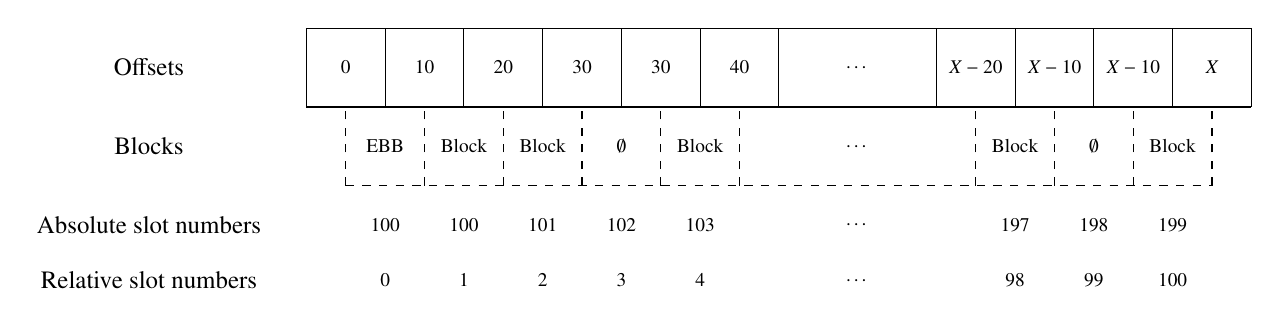
\begin{tikzpicture}
\draw (0, 0)  -- (12, 0);
\draw (0, 1)  -- (12, 1);

\draw ( 0, 0) -- ( 0, 1);
\draw ( 1, 0) -- ( 1, 1);
\draw ( 2, 0) -- ( 2, 1);
\draw ( 3, 0) -- ( 3, 1);
\draw ( 4, 0) -- ( 4, 1);
\draw ( 5, 0) -- ( 5, 1);
\draw ( 6, 0) -- ( 6, 1);
\draw ( 8, 0) -- ( 8, 1);
\draw ( 9, 0) -- ( 9, 1);
\draw (10, 0) -- (10, 1);
\draw (11, 0) -- (11, 1);
\draw (12, 0) -- (12, 1);

\draw (-2.0, 0.5) node {\small Offsets};
\draw ( 0.5, 0.5) node {\scriptsize  0};
\draw ( 1.5, 0.5) node {\scriptsize 10};
\draw ( 2.5, 0.5) node {\scriptsize 20};
\draw ( 3.5, 0.5) node {\scriptsize 30};
\draw ( 4.5, 0.5) node {\scriptsize 30};
\draw ( 5.5, 0.5) node {\scriptsize 40};
\draw ( 7.0, 0.5) node {\scriptsize \ldots};
\draw ( 8.5, 0.5) node {\scriptsize $X - 20$};
\draw ( 9.5, 0.5) node {\scriptsize $X - 10$};
\draw (10.5, 0.5) node {\scriptsize $X - 10$};
\draw (11.5, 0.5) node {\scriptsize $X$};

\draw[dashed] (0.5, -1) -- (11.5, -1);

\draw[dashed] ( 0.5, -1) -- ( 0.5, 0);
\draw[dashed] ( 1.5, -1) -- ( 1.5, 0);
\draw[dashed] ( 2.5, -1) -- ( 2.5, 0);
\draw[dashed] ( 3.5, -1) -- ( 3.5, 0);
\draw[dashed] ( 4.5, -1) -- ( 4.5, 0);
\draw[dashed] ( 5.5, -1) -- ( 5.5, 0);
\draw[dashed] ( 8.5, -1) -- ( 8.5, 0);
\draw[dashed] ( 9.5, -1) -- ( 9.5, 0);
\draw[dashed] (10.5, -1) -- (10.5, 0);
\draw[dashed] (11.5, -1) -- (11.5, 0);

\draw (-2.0, -0.5) node {\small Blocks};
\draw ( 1.0, -0.5) node {\scriptsize EBB};
\draw ( 2.0, -0.5) node {\scriptsize Block};
\draw ( 3.0, -0.5) node {\scriptsize Block};
\draw ( 4.0, -0.5) node {\scriptsize $\emptyset$};
\draw ( 5.0, -0.5) node {\scriptsize Block};
\draw ( 7.0, -0.5) node {\scriptsize \ldots};
\draw ( 9.0, -0.5) node {\scriptsize Block};
\draw (10.0, -0.5) node {\scriptsize $\emptyset$};
\draw (11.0, -0.5) node {\scriptsize Block};

\draw (-2.0, -1.5) node {\small Absolute slot numbers};
\draw ( 1.0, -1.5) node {\scriptsize 100};
\draw ( 2.0, -1.5) node {\scriptsize 100};
\draw ( 3.0, -1.5) node {\scriptsize 101};
\draw ( 4.0, -1.5) node {\scriptsize 102};
\draw ( 5.0, -1.5) node {\scriptsize 103};
\draw ( 7.0, -1.5) node {\scriptsize \ldots};
\draw ( 9.0, -1.5) node {\scriptsize 197};
\draw (10.0, -1.5) node {\scriptsize 198};
\draw (11.0, -1.5) node {\scriptsize 199};

\draw (-2.0, -2.2) node {\small Relative slot numbers};
\draw ( 1.0, -2.2) node {\scriptsize 0};
\draw ( 2.0, -2.2) node {\scriptsize 1};
\draw ( 3.0, -2.2) node {\scriptsize 2};
\draw ( 4.0, -2.2) node {\scriptsize 3};
\draw ( 5.0, -2.2) node {\scriptsize 4};
\draw ( 7.0, -2.2) node {\scriptsize \ldots};
\draw ( 9.0, -2.2) node {\scriptsize 98};
\draw (10.0, -2.2) node {\scriptsize 99};
\draw (11.0, -2.2) node {\scriptsize 100};

\end{tikzpicture}
\end{center}

The version number we mentioned above can be used to migrate indices in the old
format to a newer format, when the need would arise in the future. We do not
include a version number in the secondary index, as both index formats are
tightly coupled, which means that both index files should be migrated together.

One might realise that because the size of a secondary index entry is static,
the primary index could be represented more compactly using a bitmap. This is
indeed the case and the reason for it not being a bitmap is mostly a historical
accident. However, this accident has the upside that migrating to variable-sized
secondary index entries, e.g., serialised using CBOR instead of
\lstinline!Binary! is straightforward.

\paragraph{Lookup}

Having discussed both index formats, we can now finally detail the process of
looking up a block by a point. Given a point with slot $s$ and hash $h$, we need
to go through the following steps to read the corresponding block:

\begin{enumerate}
\item Determine the chunk number $c = \chunkNumber{s}$.
\item Determine the relative slot $\mathit{rs}$ within chunk $c$ corresponding
  to $s$: $\mathit{rs} = \relativeSlot{s}{\mathit{isEBB}}$.

  Note the $\mathit{isEBB}$ argument, which is unknown at this point. Just by
  looking at the slot and the static chunk size, we can tell whether the block
  \emph{could} be an EBB or not: only the very first slot in a chunk (which has
  the same size as a Byron epoch) could correspond to an EBB \emph{or} the
  regular block after it. For all other slots we are certain they cannot
  correspond to an EBB.

  In case the slot $s$ corresponds to the very first slot in the chunk, we will
  have to use the hash $h$ to determine whether the point corresponds to the EBB
  or the regular block in slot $s$.
\item We lookup the offset at $\mathit{rs}$ and the offset after it in the
  primary index of chunk $c$. As discussed, these lookups go through a cache and
  are cheap. We now have the offsets in the secondary index file corresponding
  to the start and end of the secondary index entry we are interested in. If
  both offsets are equal, the slot is empty, and the lookup process terminates.

  In case of a potential EBB, we have to do two such lookups: once for relative
  slot 0 and once for relative slot 1.

\item We read the secondary index entry from the secondary index file. The
  secondary indices are also cached on a per chunk basis. The secondary index
  entry contains the header hash, which we can now compare against $h$. In case
  of a match, we can read the block from the chunk file using the block offset
  contained in the secondary index entry. When the hash does not match, the
  lookup process terminates.

  In case of a potential EBB, the hash comparisons finally tell us whether the
  point corresponds to the EBB or the regular block in slot $s$, or
  \emph{neither} in case both hashes do not match $h$.
\end{enumerate}

\subsection{Recovery}
\label{immutable:implementation:recovery}

Because of the specific requirements of the Immutable DB and the expected write
patterns, we can use a much simpler recovery scheme than traditional database
systems. Only the immutable, append-only part of the chain is stored, which
means that data inconsistencies (e.g., because of a hard shutdown) are most
likely to happen at the end of the chain, i.e., in the last chunk and its
indices. We can simply truncate the chain in such cases. As we maintain some
overlap with the Volatile DB\todo{link}, blocks truncated from the end of the
chain are likely to still be in the Volatile DB, making the recovery process
unnoticeable. If the overlap is not enough and the truncated blocks are not in
the Volatile DB, they can simply be downloaded again.

There are two modes of recovery:
\begin{enumerate}
\item Validate the last chunk: this is the default mode when opening the
  Immutable DB. The last chunk file and its indices are validated. This will
  detect and truncate append operations that did not go through entirely, e.g.,
  a block that was only partially appended to a chunk file, or a block that was
  appended to one or both of the indices, but not to the chunk file.

  When after truncating a chunk file, the chunk file becomes empty, we validate
  the chunk file before it. In the unlikely case that that chunk file has to be
  truncated and ends up empty too, we validate the chunk file before it and so
  on, until we reach a valid block or the database is empty.

\item Validate all chunks: this is the full recovery mode that is triggered by a
  dirty shut down, caused by a missing or corrupted file (e.g., a checksum
  mismatch while reading), or because the node itself was not shut down
  properly.\todo{In the latter case, validating the last would be enough} We
  validate all chunk files and their indices, from oldest to newest. When a
  corrupt or missing block is encountered, we truncate the chain to the last
  valid block before it. Trying to recover from a chain with holes in it would
  be terribly complex, we therefore do not even try it.

\end{enumerate}
In both recovery modes, chunks are validated the same way, which we will shortly
describe. When in full recovery mode, we also check whether the last block in a
chunk is the predecessor of the first block in the next chunk, by comparing the
hashes. This helps sniff out a truncated chunk file that is not the final one,
causing a gap in the chain.

Validating a chunk proceeds as follows:
\begin{itemize}
\item In the common case, the chunk file and the corresponding primary and
  secondary index files will be present and all valid. We optimise for this
  case.\footnote{Unlike in other areas, where we try to maintain that the
  average case is equal to the worst case.}

\item The secondary index contains a CRC32 checksum of each block in the
  corresponding chunk (see \cref{immutable:implementation:indices}), we extract
  these checksums and pass them to the \emph{chunk file parser}.

\item The chunk file parser will try to deserialise all blocks in a chunk file.
  When a block fails to deserialise, it is treated as corrupt and we truncate
  the chain to the last valid block before it. Each raw block is also checked
  against the CRC32 checksum from the secondary index, to detect corruptions
  that are not caught by deserialising, e.g., flipping a bit in a
  \lstinline!Word64!, which can remain a valid, yet corrupt
  \lstinline!Word64!.\footnote{One might think that deserialising the blocks is
  not necessary if the checksums all match. However, the chunk file parser also
  the corresponding secondary index, which is used to validate the on-disk one.
  For this process deserialisation is required.}

  When the CRC32 checksum is not available, because of a missing or partial
  secondary index file, we fall back to the more expensive validation of the
  block based on its cryptographic hashes to detect silent corruption. This type
  of validation is block-dependent and provided in the form of the
  \lstinline!nodeCheckIntegrity! method of the \lstinline!NodeInitStorage!
  class. This validation is implemented by hashing the body of the block and
  comparing it against the body hash stored in the header, and by verifying the
  signature of the header.

  When the CRC32 checksum \emph{is} available, but does not match the one
  computed from the raw block, we also fall back to this validation, as we do
  not know whether the checksum or the block was corrupted (although the latter
  is far more likely).

  The chunk file parser also verifies that the hashes line up within a chunk, to
  detect missing blocks. It does this by comparing the ``previous hash'' of each
  block with the previous block's hash.

  The chunk file parser returns a list of secondary index entries, forming
  together the corresponding secondary index.

\item The chunk file containing the blocks is our source of truth. To check the
  validity of the secondary index, we check whether it matches the secondary
  index returned by the chunk file parser. If there is a mismatch, we overwrite
  the entire secondary index file using the secondary index returned by the
  chunk file parser.

\item We can reconstruct the primary index from the secondary index returned by
  the chunk file parser. When the on-disk primary index is missing or it is not
  equal to the reconstructed one, we (over)write it using the reconstructed one.

\item When truncating the chain, we always make sure that the resulting chain
  ends with a block, i.e., a filled slot, not an empty slot. Even if this means
  going back to the previous chunk.

\end{itemize}

We test the recovery process in our \lstinline!quickcheck-state-machine! tests
of the Immutable DB. In various states of the Immutable DB, we generate one or
more random corruptions for any of the on-disk files: either a simple deletion
of the file, a truncation, or a random bitflip. We verify that after restarting
the Immutable DB, it has recovered to the last valid block before the
truncation.

Additionally, in those same tests, we simulate file-system errors during
operations. For example, while appending a block, we let the second disk write
fail. This is another way of testing whether we can correctly recover from a
write that was aborted half-way through.

\chapter{Volatile Database}
\label{volatile}

\chapter{Ledger Database}
\label{ledgerdb}

\section{Initialisation}
\label{ledgerdb:initialisation}

Describe why it is important that we store a single snapshot and then replay
ledger events to construct the ledger DB.

\newcommand{\chainle}{\ensuremath{\mathrel{\sqsubseteq}}}
\newcommand{\chainlt}{\ensuremath{\mathrel{\sqsubset}}}
\newcommand{\chainnotlt}{\ensuremath{\mathrel{\nsqsubset}}}
\newcommand{\wehave}{.\;}
\newcommand{\suchthat}{.\;}
\newcommand{\app}{\ensuremath{\mathrel{\triangleright}}}
\newcommand{\length}[1]{\ensuremath{\mathrm{length} \; #1}}
\newcommand{\ifthen}[2]{\ensuremath{\mathrm{if} \quad #1 \quad \mathrm{then} \quad #2}}
\renewcommand{\iff}{\ensuremath{\qquad\mathrm{iff}\qquad}}
\newcommand{\candidates}[2]{\ensuremath{\mathsf{candidates}_#1(#2)}}
\newcommand{\blockNo}[1]{\ensuremath{\mathtt{blockNo}(#1)}}
\newcommand{\selectviewle}{\ensuremath{\precsim}}

\chapter{Chain Selection}
\label{chainsel}

Chain selection is one of the central responsibilities of the chain database
(\cref{chaindb}). It of course depends on chain selection as it is defined  by
the consensus protocol (\cref{consensus:class:chainsel}), but needs to  take
care of a lot of operational concerns. In this chapter we will take a closer
look at the implementation of chain selection in the chain database, and state
some properties and sketch some proofs to motivate it.

\section{Comparing anchored fragments}
\label{chainsel:fragments}

\subsection{Introduction}

Recall from \cref{consensus:overview:chainsel} that while in the literature
chain selection is defined in terms of comparisons between entire chains, we
instead opted to model it in terms of a comparison between the \emph{headers} at
the tip of those chains (or rather, a \emph{view} on those headers defined by
the specific consensus protocol).

We saw in \cref{storage:inmemory} (specifically, \cref{storage:fragments}) that
the consensus layer stores chain fragments in memory (the most recent headers on
a chain), both for the node's own current chain as well as for upstream nodes
(which we refer to as ``candidate chains''). Defining chain selection in terms
of fragments is straight-forward when those fragments are non-empty: we simply
take the most recent header, extract the view required by the consensus protocol
(\cref{BlockSupportsProtocol}), and then use the consensus protocol's chain
selection interface to compare them. The question is, however, how to compare
two fragments when one (or both) of them is \emph{empty}. This problem is more
subtle than it might seem at first sight, and requires careful consideration.

We mentioned in \cref{consensus:overview:chainsel} that consensus imposes a
fundamental assumption that the strict extension of a chain is always (strictly)
preferred over that chain (\cref{prefer-extension}), and that consequently we
\emph{always} prefer a non-empty chain over an empty one (and conversely we
\emph{never} prefer an empty chain over a non-empty one). However, chain
fragments are mere proxies for their chains, and the fragment might be empty
even if the chain is not. This means that in principle it's possible we do not
prefer a non-empty fragment over an empty one, or indeed prefer an empty
fragment over a non-empty one. However, when a fragment is empty, we cannot rely
on the consensus protocol's chain selection because we have no header to give
it.

Let's consider under which conditions these fragments might be empty:

\begin{description}
\item[Our fragment]
Our own fragment is a path through the volatile database, anchored at the tip of
the immutable database (\cref{storage:fragments}). Under normal circumstances,
it will be empty only if our \emph{chain} is empty; we will refer to such empty
fragments as \emph{genuinely empty}.\footnote{We can distinguish between an empty
fragment of a non-empty chain and a (necessarily) empty fragment of an empty
chain by looking at the anchor point: if it is the genesis point, the chain must
be empty.} However, our fragment can also be empty even when our chain is not,
if due to data loss the volatile database is empty (or contains no blocks that
fit onto the tip of the immutable database).

\item[Candidate fragment]
A \emph{genuinely} empty candidate fragment, representing an empty candidate
chain, is never preferred over our chain. Unfortunately, however, the candidate
fragment as maintained by the chain sync client (\cref{chainsyncclient}) can
essentially be empty at any point due to the way that a switch-to-fork is
implemented in terms of rollback followed by roll forward: after a maximum
rollback (and before the roll forward), the candidate fragment is empty.
\end{description}

\subsection{Precondition}
\label{chainsel:fragments:precondition}

Since neither of these circumstances can be avoided, we must therefore impose a
precondition for chain selection between chain fragments to be definable:

\begin{definition}[Precondition for comparing chain fragments]
The two fragments must either both be non-empty, or they must intersect.
\end{definition}

In this chapter, we establish this precondition in two different ways:

\begin{enumerate}
\item When we construct candidates chains (potential chains that we may wish
to replace our own chain with), those candidate chains must intersect with
our own chain within $k$ blocks from its tip; after all, if that is not the
case, we would induce a roll back of more than $k$ blocks
(\cref{consensus:overview:k}).

\item When we compare fragments to each other, we only compare fragments from a
set of fragments that are all anchored at the same point (i.e., the anchor of
all fragments in the set is the same, though it might be different from the
anchor of our current fragment). Since they are all anchored at the same point,
they trivially all intersect with each other.
\end{enumerate}

There is one more use of fragment selection, which is rather more subtle;
we will come back to this in \cref{chainsyncclient:plausiblecandidates}.

\todo{TODO} TODO: Throughout we are talking about \emph{anchored} fragments
here. We should make sure that we discuss those somewhere.

\subsection{Definition}
\label{chainsel:fragments:definition}

We will now show that this precondition suffices to compare two fragments,
whether or not they are empty; we'll consider each case in turn.

\begin{description}

\item[Both fragments empty]
Since the two fragments must intersect, that intersection point can only
be the two anchor points, which must therefore be equal. This means that
two fragments represent the same chain: neither fragment is preferred
over the other.

\item[First fragment non-empty, second fragment empty]
Since the two fragments must intersect, that intersection can only be the
anchor of the second fragment, which can lie anywhere on the first fragment.

\begin{itemize}
\item If it lies at the \emph{tip} of the first fragment, the two fragments represent the
same chain, and neither is preferred over the other.
\item If it lies \emph{before} the tip of first fragment, the first fragment is
a strict extension of the second, and is therefore is preferred over the
second.
\end{itemize}

\item[First fragment empty, second fragment non-empty]
This case is entirely symmetric to the previous; if the intersection is the
tip of the second fragment, the fragments represent the same chain. Otherwise,
the second fragment is a strict extension of the first, and is therefore
preferred.

\item[Both fragments non-empty]
In this case, we can simply use the consensus protocol chain selection API
to compare the two most recent headers on both fragments.

\end{description}

Note that this relies critically on the ``prefer extension'' rule
(\cref{prefer-extension}).

\section{Preliminaries}
\label{chainsel:spec}

Recall from \cref{storage:components} that the immutable database stores a
linear chain, terminating in the \emph{tip} $I$ of the immutable database. The
volatile database stores a (possibly fragmented) tree of extensions to that
chain:
%
\begin{center}
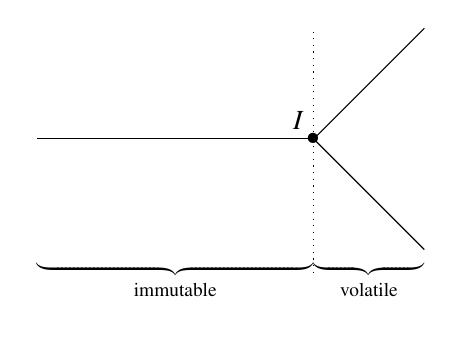
\begin{tikzpicture}
\draw (0,0) -- (100pt, 0) coordinate (immtip) node{$\bullet$} node[above left] {$I$};
\draw (immtip) -- ++(40pt,  40pt);
\draw (immtip) -- ++(40pt, -40pt);
\draw [dotted] (immtip) -- ++(0, 40pt);
\draw [dotted] (immtip) -- ++(0, -50pt);
\node at (50pt, -40pt) [below] {$\underbrace{\hspace{100pt}}_\textrm{immutable}$};
\node at (120pt, -40pt) [below] {$\underbrace{\hspace{40pt}}_\textrm{volatile}$};
\end{tikzpicture}
\end{center}
%
The node's \emph{current chain} is stored in memory as a chain fragment through
the volatile database, anchored at $I$.  When we start up the node, the chain
database must find the best possible path through the volatile database and
adopt that as our current fragment; every time a new block is added to the
volatile database, we have to recompute the new best possible path. In other
words, we maintain the following invariant:

\begin{definition}[Current chain invariant]
\label{current-chain-invariant}
The current chain is the best possible path through the volatile DB.
\end{definition}

``Best'' of course is according to the chain selection rule defined by the
consensus protocol (\cref{consensus:class:chainsel}). In this section we
describe how the chain database establishes and preserves this invariant.

\subsection{Notation}

So far we have been relatively informal in our description of chain selection,
but in order to precisely describe the algorithm and state some of its
properties, we have to introduce some notation.

\begin{definition}[Chain selection]
We will model chain selection as a transitive binary relation (\chainlt) between
valid chains (it is undefined for invalid chains), and let $C \chainle C'$ if
and only if $C \chainlt C'$ or $C = C'$. It follows that (\chainle) is a partial
order (reflexive, antisymmetric, and transitive).
\end{definition}

For example, the simple ``prefer longest chain'' chain selection rule could be
given as
%
\begin{equation*}
\tag{longest chain rule}
C \chainlt C'  \iff  \length{C} < \length{C'}
\end{equation*}

In general of course the exact rule depends on the choice of consensus protocol.
\Cref{prefer-extension} (\cref{consensus:overview:chainsel}) can now be
rephrased as
%
\begin{equation}
\label{eq:prefer-extension}
\forall C, B \wehave C \chainlt (C \app B)
\end{equation}

We will not be comparing whole chains, but rather chain fragments
(we will leave the anchor of fragments implicit):
%
\begin{definition}[Fragment selection]
We lift $\chainlt$ to chain fragments in the manner described in
\cref{chainsel:fragments}; this means that $\chainlt$ is undefined for two
fragments if they do not intersect (\cref{chainsel:fragments:precondition}).
\end{definition}

We also lift $\chainle$ to \emph{sets} of fragments, intuitively indicating that
a particular fragment is the ``best choice'' out of a set $\mathcal{S}$ of
candidate fragments:
%
\begin{definition}[Optimal candidate]
\begin{equation*}
\mathcal{S} \chainle F  \iff   \nexists F' \in \mathcal{S} \suchthat F \chainlt F'
\end{equation*}
(in other words, if additionally $F \in \mathcal{S}$, then $F$ is a maximal
element of $C$). This inherits all the preconditions of $\chainle$ on chains and
fragments.
\end{definition}

Finally, we will introduce some notation for \emph{computing} candidate
fragments:\footnote{In order to compute these candidates efficiently, the
volatile database must support a ``forward chain index'', able to efficiently
answer the question ``which blocks succeed this one?''.}

\begin{definition}[Construct set of candidates]
Given some set of blocks $V$, and some anchor $A$ (with $A$ either a block or
the genesis point), $$\candidates{A}{V}$$ is the set of chain fragments
anchored at $A$ using blocks picked from $V$.
\end{definition}

By construction all fragments in $\candidates{A}{V}$ have the same anchor, and
hence all intersect (at $A$); this will be important for the use of the
$\chainle$ operator.

\subsection{Properties}

In the following we will use ($F \app B$) to denote appending block $B$ to chain
$F$, and lift this notation to sets, so that for some set of blocks
$\mathcal{B}$ we have
%
\begin{equation*}
F \app \mathcal{B} = \{ F \app B \mid B \in \mathcal{B} \}
\end{equation*}

\begin{lemma}[Properties of the set of candidates]
\label{candidates:properties}
The set of candidates computed by $\candidates{A}{V}$ has the following
properties.

\begin{enumerate}

\item \label{candidates:prefixclosed}
It is prefix closed:
\begin{equation*}
\forall F, B \wehave
\ifthen
  {(F \app B) \in \candidates{A}{V}}
  {F \in \candidates{A}{V}}
\end{equation*}

\item \label{candidates:appendnew}
If we add a new block into the set, we can append that block to existing
candidates (where it fits):
\begin{equation*}
\ifthen
  {F \in \candidates{A}{V}}
  {F \app B \in \candidates{A}{V \cup \{ B \}}}
\end{equation*}
provided $F$ can be extended with $B$.

\item \label{candidates:monotone}
Adding blocks doesn't remove any candidates:
\begin{equation*}
\candidates{A}{V} \subseteq \candidates{A}{V \cup \{B\}}
\end{equation*}

\item \label{candidates:musthavenew}
If we add a new block, then any new candidates must involve that new block:
\begin{equation*}
\ifthen
  {F \in \candidates{A}{V \cup \{B\}}}
  {F \in \candidates{A}{V} \text{ or } F = (\ldots \app B \app \ldots)}
\end{equation*}

\end{enumerate}
\end{lemma}

The next lemma says that if we have previously found some optimal candidate $F$,
and subsequently learn of a new block $B$ (where $B$ is a direct or indirect
extension of $F$), it suffices to find a locally optimal candidate \emph{amongst
the candidates that involve $B$}; this new candidate will also be a globally
optimal candidate.

\begin{lemma}[Focus on new block]
\label{focusonnewblock}
Suppose we have $F, F_\mathit{new}$ such that
\begin{enumerate}
\item \label{focusonnewblock:previouslyoptimal}
$\candidates{A}{V} \chainle F$
\item \label{focusonnewblock:optimalamongstnew}
$(\candidates{A}{V \cup \{B\}} \setminus \candidates{A}{V}) \chainle F_\mathit{new}$
\item \label{focusonnewblock:betterthanold}
$F \chainle F_\mathit{new}$
\end{enumerate}
Then
\begin{equation*}
\candidates{A}{V \cup \{B\}} \chainle F_\mathit{new}
\end{equation*}
\end{lemma}

\begin{proof}
Suppose there exists $F' \in \candidates{A}{V \cup \{B\}}$ such that
$F_\mathit{new} \chainlt F'$. By transitivity and
assumption~\ref{focusonnewblock:betterthanold}, $F \chainlt F'$. As
shown in \cref{candidates:properties} (\cref{candidates:musthavenew}), there are two possibilities:

\begin{itemize}
\item $F' \in \candidates{A}{V}$, which would violate
assumption~\cref{focusonnewblock:previouslyoptimal}, or
\item $F'$ must contain block $B$, which would violate
assumption~\cref{focusonnewblock:optimalamongstnew}.
\end{itemize}
\end{proof}

\section{Initialisation}
\label{chainsel:init}

The initialisation of the chain database proceeds as follows.

\begin{enumerate}

\item
\label{chaindb:init:imm}
Initialise the immutable database, determine its tip $I$, and ask the ledger DB
for the corresponding ledger state $L$ (see
\cref{ledgerdb:on-disk:initialisation}).

\item Compute the set of candidates anchored at the immutable database's tip
\label{chaindb:init:compute}
$I$ using blocks from the volatile database $V$
$$\candidates{I}{V}$$
ignoring known-to-be-invalid blocks (if any; see \cref{chaindb:invalidblocks})
and order them using $(\chainlt)$  so that we process better candidates
first.\footnote{Technically speaking we should \emph{first} validate all
candidates, and only then apply selection to the valid chains. We perform chain
selection first, because that is much cheaper. Both approaches are semantically
equivalent, since \lstinline!sortBy f . filter p = filter p . sortBy f! due to
the stability of \lstinline!sortBy!.} Candidates that are strict prefixes of
other candidates can be ignored (as justified by the ``prefer extension''
assumption, \cref{prefer-extension});\footnote{The implementation does not
compute candidates, but rather ``maximal'' candidates, which do not include such
prefixes.} we may reconsider some of these prefixes if we subsequently discover
invalid blocks (see \cref{chaindb:init:select}).

\item
\label{chaindb:init:select}
Not all of these candidates may be valid, because the volatile database stores
blocks whose \emph{headers} have been validated, but whose \emph{bodies} are
still unverified (other than to check that they correspond to their headers).
We therefore validate each candidate chain fragment, starting with $L$ (the
ledger state at the tip of the immutable database) each time.\footnote{We make
no attempt to share ledger states between candidates, even if they share a
common prefix, trading runtime performance for lower memory pressure.}

As soon as we find a candidate that is valid, we adopt it as our current chain.
If we find a candidate that is \emph{invalid}, we mark the invalid
block\footnote{There is no need to mark any successors of invalid blocks; see
\cref{chaindb:dont-mark-invalid-successors}.} (unless it is invalid due to
potential clock skew, see \cref{chainsel:infuture}), and go back to
step~\ref{chaindb:init:compute}. It is important to recompute the set of
candidates after marking some blocks as invalid because those blocks may also
exist in other candidates and we do not know how the valid prefixes of those
candidates should now be ordered.

\end{enumerate}

\section{Adding new blocks}
\label{chainsel:addblock}

When a new block $B$ is added to the chain database, we need to add it to the
volatile DB and recompute our current chain. We distinguish between the
following different cases.

Before we process the new block, we first run chain selection on any blocks that
had previously been temporarily shelved because their slot number was (just)
ahead of the wallclock (\cref{chainsel:infuture}). We do this independent of what
we do with the new block.\footnote{In a way, calls to \lstinline!addBlock! are
how the chain database sees time advance. It does not rely on slot length to do
so, because slot length is ledger state dependent.}

The implementation \lstinline!addBlock! additionally provides  client code with
various notifications throughout the process  (``block added'', ``chain
selection run'', etc.). We will not describe these notifications here.

\subsection{Ignore}

We can just ignore the block if any of the following is true.

\begin{itemize}

\item
The block is already in the immutable DB, \emph{or} it belongs to a branch which
forks more than $k$ blocks away from our tip, i.e.\footnote{The check is a
little more complicated in the presence of EBBs (\cref{ebbs}). This is relevant
if we switch to an alternative fork after a maximum rollback, and that
alternative fork starts with an EBB. It is also relevant when due to data
corruption the volatile database is empty and the first block we add when we
continue to sync the chain happens to be an EBB.}
%
\begin{equation*}
\blockNo{B} \leq \blockNo{I}
\end{equation*}
%
We could distinguish between between the block being on our chain or on a
distant fork by doing a single query on the immutable database, but it does not
matter: either way we do not care about this block.

We don't expect the chain sync client to feed us such blocks under normal
circumstances, though it's not impossible: by the time a block is downloaded
it's conceivable, albeit unlikely, that that block is now older than $k$.

\item
The block was already in the volatile database, i.e.
%
\begin{equation*}
B \in V
\end{equation*}

\item
The block is known to be invalid (\cref{chaindb:invalidblocks}).

\end{itemize}

\subsection{Add to current chain}
\label{chainsel:addtochain}

Let $B_\mathit{pred}$ be the predecessor block of $B$. If $B$ fits onto the end
of our current fragment $F$ (and hence onto our current chain) $F$, i.e.
%
\begin{itemize}
\item $F$ is empty, and $B_\mathit{pred} = I$
(where $I$ must necessarily also be the anchor of the fragment), or
\item $\exists F' \suchthat F = F' \app B_\mathit{pred}$
\end{itemize}
%
then any new candidates must be equal to or an extension of $F \app B$
(\cref{candidates:properties}, \cref{candidates:musthavenew}); this set is
computed by
%
\begin{equation*}
(F \app B \app \candidates{B}{V \cup \{B\}})
\end{equation*}
%
Since all candidates would be strictly preferred over $F$ (since they are
extensions of $F$), by \cref{focusonnewblock} it suffices to pick the best
candidate amongst these extensions. Apart from the starting point, chain
selection then proceeds in the same way as when we are initialising the database
(\cref{chainsel:init}).

This case takes care of the common case where we just add a block to our chain,
as well as the case where we stay with the same branch but receive some blocks
out of order. Moreover, we can use the \emph{current} ledger state as the
starting point for validation.

\subsection{Store, but don't change current chain}

When we are missing one of the (transitive) predecessors of the block, we store
the block but do nothing else. We can check this by following back pointers
until we reach a block $B'$ such that $B' \notin V$ and $B' \neq I$. The cost of
this is bounded by the length of the longest fragment in the volatile DB, and
will typically be low; moreover, the chain fragment we are constructing this way
will be used in the switch-to-fork case
(\cref{chainsel:switchtofork}).\footnote{The function that constructs these
fragments is called \lstinline!isReachable!.}

At this point we \emph{could} do a single query on the immutable DB to check if
$B'$ is in the immutable DB or not. If it is, then this block is on a distant
branch that we will never switch to, and so we can ignore it. If it is not, we
may or may not need this block later and we must store it; if it turns out we
will never need it, it will eventually be garbage collected (\cref{chaindb:gc}).

An alternative and easier approach is to omit the check on the immutable DB,
simply assuming we might need the block, and rely on garbage collection to
eventually remove it if we don't. This is the approach we currently use.

\subsection{Switch to a fork}
\label{chainsel:switchtofork}

If none of the cases above apply, we have a block $B$ such that

\begin{enumerate}
\item \label{chainsel:switchtofork:notinvoldb}
$B \notin V$
\item \label{chainsel:switchtofork:notinimmdb}
$\blockNo{B} > \blockNo{I}$ (and hence $B$ cannot be in the immutable DB)
\item \label{chainsel:switchtofork:connected}
For all transitive predecessors $B'$ of $B$ we have $B' \in V$ or $B' = I$.
In other words, we must have a fragment
$$F_\mathit{prefix} = I \app \ldots \app B$$
in $\candidates{I}{V \cup \{B\}}$.
\item \label{chainsel:switchtofork:doesnotfit}
(Either $F$ is empty and $B_\mathit{pred} \neq I$, or) $\exists F', B' \suchthat
F = F' \app B'$ where $B' \neq B_\mathit{pred}$; i.e., block does not fit onto
current chain.\footnote{\Cref{chainsel:switchtofork:connected} rules out the
first option: if $B_\mathit{pred} \neq I$ then we must have $B_\mathit{pred} \in
V$ and moreover this must form some kind of chain back to $I$; this means that
the preferred candidate cannot be empty.}
\end{enumerate}

(This list is just the negation of the conditions we handled in the sections
above.)
We proceed in similar fashion to the case when the block fit onto the tip of our
chain (\cref{chainsel:addtochain}). The new candidates in $\candidates{I}{V \cup
\{B\}}$ must involve $B$ (\cref{candidates:properties},
\cref{candidates:musthavenew}), which in this case means they must all be
extensions of $F_\mathit{prefix}$; we can compute these candidates
using\footnote{The implementation of the chain database actually does not
construct fragments that go back to $I$, but rather to the intersection point
with the current chain. This can be considered to be an optimisation of what we
describe here.}
$$I \app \ldots \app B \app \candidates{B}{V \cup \{B\}}$$
Not all of these fragments might be preferred over the current chain; we filter
those out.\footnote{Recall that the current chain gets special treatment: when
two candidates are equally preferable, we can pick either one, but when a
candidate and the current chain are equally preferable, we must stick with the
current chain.} We then proceed as usual, considering each of the remaining
fragments in $(\chainle)$ order, and appeal to \cref{focusonnewblock}
again to conclude that the fragment we find in this way will be an optimal
candidate across the entire volatile database.


%
% *
%
% *
%
%
% It is worth pointing out that we do _not_ rely on `F_prefix` being longer than
% the current chain. Indeed, it may not be: if two leaders are selected for the
% same slot, and we _receive_ a block for the current slot before we can _produce_
% one, our current chain will contain the block from the other leader; when we
% then produce our own block, we end up in the switch-to-fork case; here it is
% important that `preferCandidate` would prefer a candidate chain (the chain that
% contains our own block) over our current chain, even if they are of the same
% length, if the candidate ends in a block that we produced (and the current chain
% does not); however, the `ChainDB` itself does not need to worry about this
% special case.
%
% [let's be explicit about the difference between current chain and self
% produced blocks]
%

\section{In-future check}
\label{chainsel:infuture}

As we saw in \cref{chainsel:spec}, the chain DB performs full
block validation during chain selection. When we have validated a block, we then
do one additional check, and verify that the block's slot number is not ahead of
the wallclock time (for a detailed discussion of why we require the block's
ledger state for this, see \cref{time}, especially
\cref{time:block-infuture-check}). If the block is far ahead of the wallclock,
we treat this as any other validation error and mark the block as invalid.

Marking a block as invalid will cause the network layer to disconnect from the
peer that provided the block to us, since non-malicious (and non-faulty) peers
should never send invalid blocks to us. It is however possible that an upstream
peer's clock is not perfectly aligned with us, and so they might produce a block
which \emph{we} think is ahead of the wallclock but \emph{they} do not. To avoid
regarding such peers as malicious, the chain database supports a configurable
\emph{permissible clock skew}: blocks that are ahead of the wallclock by an
amount less than this permissible clock skew are not marked as invalid, but
neither will chain selection adopt them; instead, they simply remain in the
volatile database available for the next chain selection.

It is constructive to consider what happens if \emph{our} clock is off, in
particular, when it is slow. In this scenario \emph{every} (or almost every)
block that the node receives will be considered to be in the future. Suppose we
receive two consecutive blocks $A$ and $B$. When we receive $A$, chain selection
runs, we find that $A$ is ahead of the clock but within the permissible clock
skew, and we don't adopt it. When we then receive $B$, chain selection runs
again, we now discover the $A, B$ extension to our current chain; during
validation we cut off this chain at $B$ because it is ahead of the clock, but we
adopt $A$ because it is now valid.  In other words, we are always behind one
block, adopting each block only when we receive the \emph{next} block.

\begin{bug}
One problem with this scheme is that if we receive a block $B$ which is ahead of
the clock when we receive it, we might never notice it if block $B$ is not (yet)
connected to our chain: by the time we receive the missing blocks (which connect
$B$ to our chain), $B$ might no longer be ahead of the clock and we might adopt
it, even if $B$ was ahead by more than the permissible clock skew.

We could avoid this problem if we stored the time we received a block alongside
the block in the volatile database, but in the current design, the volatile
database does not store \emph{any} information on disk apart from raw blocks,
so this would be quite a significant design change.
\end{bug}

\section{Sorting}

In this chapter we have modelled chain selection as a partial order
$(\chainle)$. This suffices for the formal treatment, and in theory also
suffices for the implementation. However, at various points during the chain
selection process we need to \emph{sort} candidates in order of preference. We
can of course sort values based on a preorder only (topological sorting), but we
can do slightly better. Recall from \cref{consensus:class:chainsel} that we
require that the \lstinline!SelectView! on headers must be a total order. We can
therefore define

\begin{definition}[Same select view]
Let $C \selectviewle C'$ if the select view at the tip of $C$ is less than
or equal to the select view at the tip of $C'$.
\end{definition}

(\selectviewle) forms a total preorder (though not a partial order); if $C
\selectviewle C'$ \emph{and} $C' \selectviewle C$ then the select views at the
tips of $C$ and $C'$ are equal (though they might be different chains, of
course). Since $C \selectviewle C'$ implies $C' \chainnotlt C$, we can use this
preorder  to sort candidates (in order words, we will sort them \emph{on} their
select view, in Haskell-parlance).

\chapter{Chain Database}
\label{chaindb}

TODO\todo{TODO}: This is currently a disjoint collection of snippets.

\section{Union of the Volatile DB and the Immutable DB}
\label{chaindb:union}

As discussed in \cref{storage:components}, the blocks in the Chain DB are
divided between the Volatile DB (\cref{volatile}) and the Immutable DB
(\cref{immutable}). Yet, it presents a unified view of the two databases.
Whereas the Immutable DB only contains the immutable chain and the Volatile DB
the volatile \emph{parts} of multiple forks, by combining the two, the Chain DB
contains multiple forks.

\subsection{Looking up blocks}
\label{chaindb:union:lookup}

Just like the two underlying databases the Chain DB allows looking up a
\lstinline!BlockComponent! of a block by its point. By comparing the slot number
of the point to the slot of the immutable tip, we could decide in which database
to look up the block. However, this would not be correct: the point might have a
slot older than the immutable tip, but refer to a block not in the Immutable DB,
i.e., a block on an older fork. More importantly, there is a potential race
condition: between the time at which the immutable tip was retrieved and the
time the block is retrieved from the Volatile DB, the block might have been
copied to the Immutable DB and garbage collected from the Volatile DB, resulting
in a false negative. Nevertheless, the overlap between the two makes this
scenario very unlikely.

For these reasons, we look up a block in the Chain DB as follows. We first look
up the given point in the Volatile DB. If the block is not in the Volatile DB,
we fall back to the Immutable DB. This means that if, at the same, a block is
copied from the Volatile DB to the Immutable DB and garbage collected from the
Volatile DB, we will still find it in the Immutable DB. Note that failed lookups
in the Volatile DB are cheap, as no disk access is required.

\subsection{Iterators}
\label{chaindb:union:iterators}

Similar to the Immutable DB (\cref{immutable:api:iterators}), the Chain DB
allows streaming blocks using iterators. We only support streaming blocks from
the current chain or from a recent fork. We \emph{do not} support streaming from
a fork that starts before the current immutable tip, as these blocks are likely
to be garbage collected soon. Moreover, it is of no use to us to serve another
node blocks from a fork we discarded.

We might have to stream blocks from the Immutable DB, the Volatile DB, or from
both. If the end bound is older or equal to the immutable tip, we simply try to
open an Immutable DB iterator with the given bounds. If the end bound is newer
than the immutable tip, we construct a path of points (see
\lstinline!filterByPredecessor! in \cref{volatile:api}) connecting the end bound
to the start bound. This path is either entirely in the Volatile DB or it is
partial because a block is missing from the Volatile DB. If the missing block is
the tip of the Immutable DB, we will have to stream from the Immutable DB in
addition to the Volatile DB. If the missing block is not the tip of the
Immutable DB, we consider the range to be invalid. In other words, we allow
streaming from both databases, but only if the immutable tip is the transition
point between the two, it cannot be a block before the tip, as that would mean
the fork is too old.

\todo{TODO} Image?

To stream blocks from the Volatile DB, we maintain the constructed path of
points as a list in memory and look up the corresponding block (component) in
the Volatile DB one by one.

Consider the following scenario: we open a Chain DB iterator to stream the
beginning of the current volatile chain, i.e., the blocks in the Volatile DB
right after the immutable tip. However, before streaming the iterator's first
block, we switch to a long fork that forks off all the way back at our immutable
tip. If that fork is longer than the previous chain, blocks from the start of
our chain will be copied from the Volatile DB to the Immutable DB,\todo{link}
advancing the immutable tip. This means the blocks the iterator will stream are
now part of a fork older than $k$. In this new situation, we would not allow
opening an iterator with the same range as the already-opened iterator. However,
we do allow streaming these blocks using the already opened iterator, as the
blocks to stream are unlikely to have already been garbage collected.
Nevertheless, it is still theoretically possible\footnote{This is unlikely, as
there is a delay between copying and garbage collection (see
\cref{chaindb:gc:delay}) and there are network time-outs on the block fetch
protocol, of which the server-side (see \cref{servers:blockfetch}) is the
primary user of Chain DB iterators.} that such a block has already been garbage
collected. For this reason, the Chain DB extends the Immutable DB's
\lstinline!IteratorResult! type (see \cref{immutable:api:iterators}) with the
\lstinline!IteratorBlockGCed! constructor:
%
\begin{lstlisting}
data IteratorResult blk b =
    IteratorExhausted
  | IteratorResult b
  | IteratorBlockGCed (RealPoint blk)
\end{lstlisting}

There is another scenario to consider: we stream the blocks from the start of
the current volatile chain, just like in the previous scenario. However, in this
case, we do not switch to a fork, but our chain is extended with new blocks,
which means blocks from the start of our volatile chain are copied from the
Volatile DB to the Immutable DB. If these blocks have been copied and garbage
collected before the iterator is used to stream them from the Volatile DB (which
is unlikely, as explained in the previous scenario), the iterator will
incorrectly yield \lstinline!IteratorBlockGCed!. Instead, when a block that was
planned to be streamed from the Volatile DB is missing, we first look in the
Immutable DB for the block in case it has been copied there. After the block
copied to the Immutable has been streamed, we continue with the remaining blocks
to stream from the Volatile DB. It might be the case that the next block has
also been copied and garbage collected, requiring another switch to the
Immutable DB. In the theoretical worst case, we have to switch between the two
databases for each block, but this is nearly impossible to happen in practice.

\subsection{Followers}
\label{chaindb:union:followers}

In addition to iterators, the Chain DB also supports \emph{followers}. Unlike an
iterator, which is used to request a static segment of the current chain or a
recent fork, a follower is used to follow the \emph{current chain}. Either from
the start of from a suggested more recent point. Unlike iterators, followers are
dynamic, they will follow the chain when it grows or forks. A follower is
pull-based, just like its primary user, the chain sync server (see
\cref{servers:chainsync}). This avoids the need to have a growing queue of
changes to the chain on the server side in case the client side is slower.

The API of a follower is as follows:
%
\begin{lstlisting}
data Follower m blk a = Follower {
      followerInstruction         :: m (Maybe (ChainUpdate blk a))
    , followerInstructionBlocking :: m (ChainUpdate blk a)
    , followerForward             :: [Point blk] -> m (Maybe (Point blk))
    , followerClose               :: m ()
    }
\end{lstlisting}
%
The \lstinline!a! parameter is the same \lstinline!a! as the one in
\lstinline!BlockComponent! (see \cref{immutable:api:block-component}), as a
follower for any block component \lstinline!a! can be opened.

A follower always has an implicit position associated with it. The
\lstinline!followerInstruction! operation and its blocking variant allow
requesting the next instruction w.r.t.\ the follower's implicit position, i.e.,
a \lstinline!ChainUpdate!:
%
\begin{lstlisting}
data ChainUpdate block a =
    AddBlock a
  | RollBack (Point block)
\end{lstlisting}
%
The \lstinline!AddBlock! constructor indicates that to follow the current chain,
the follower should extend its chain with the given block (component). Switching
to a fork is represented by first rolling back to a certain point
(\lstinline!RollBack!), followed by at least as many new blocks
(\lstinline!AddBlock!) as blocks that have been rolled back. If we were to
represent switching to a fork using a constructor like:
%
\begin{lstlisting}
  | SwitchToFork (Point block) [a]
\end{lstlisting}
%
we would need to have many blocks or block components in memory at the same
time.

These operations are implemented as follows. In case the follower is looking at
the immutable part of the chain, an Immutable DB iterator is used and no
rollbacks will be encountered. When the follower has advanced into the volatile
part of the chain, the in-memory fragment containing the last $k$ headers is
used (see \cref{storage:inmemory}). Depending on the block component, the
corresponding block might have to be read from the Volatile DB.

When a new chain has been adopted during chain selection (see
\cref{chainsel:addblock}), all open followers that are looking at the part of
the current chain that was rolled back are updated so that their next
instruction will be the correct \lstinline!RollBack!. By definition, followers
looking at the immutable part of the chain will be unaffected.

By default, a follower will start from the very start of the chain, i.e., at
genesis. Accordingly, the first instruction will be an \lstinline!AddBlock! with
the very first block of the chain. As mentioned, the primary user of a follower
is the chain sync server, of which the clients in most cases already have large
parts of the chain. The \lstinline!followerForward! operation can be used in
these cases to find a more recent intersection from which the follower can
start. The client will sent a few recent points from its chain and the follower
will try to find the most recent of them that is on our current chain. This is
implemented by looking up blocks by their point in the current chain fragment
and the Immutable DB.

Followers are affected by garbage collection similarly to how iterators are
(\cref{chaindb:union:iterators}): when the implicit position of the follower is
in the immutable part of the chain, an Immutable DB iterator with a static range
is used. Such an iterator is not aware of blocks appended to the Immutable DB
since the iterator was opened. This means that when the iterator reaches its
end, we first have to check whether more blocks have been appended to the
Immutable DB. If so, a new iterator is opened to stream these blocks. If not, we
switch over to the in-memory fragment.

\section{Block processing queue}
\label{chaindb:queue}

Discuss the chain DB's block processing queue, the future/promises/events,
concurrency concerns, etc.

Discuss the problem of the effective queue size (\#2721).

\section{Marking invalid blocks}
\label{chaindb:invalidblocks}

The chain database keeps a set of hashes of known-to-be-invalid blocks.
This information is used by the chain sync client (\cref{chainsyncclient}) to
terminate connections to nodes with a chain that contains an invalid block.

\begin{lemma}
\label{chaindb:dont-mark-invalid-successors}
When the chain database discovers an invalid block $X$, it is sufficient
to mark only $X$; there is no need to additionally mark any successors of $X$.
\end{lemma}

\begin{proof}[Proof (sketch).]
The chain sync client maintains a chain fragment corresponding to some suffix
of the upstream node's chain, and it preserves an invariant that that suffix
must intersect with the node's own current chain. It can therefore never be
the case that the fragment contains a successor of $X$ but not $X$ itself:
since $X$ is invalid, the node will never adopt it, and so a fragment that
intersects the node's current chain and includes a successor of $X$ \emph{must}
also contain $X$.
\end{proof}

TODO\todo{TODO}: We should discuss how this relates to GC (\cref{chaindb:gc}).

\section{Effective maximum rollback}

The maximum rollback we can support is bound by the length of the current  fragment. This will be less than $k$ only if

\begin{itemize}
\item We are near genesis and the immutable database is empty, or
\item Due to data corruption the volatile database lost some blocks
\end{itemize}

Only the latter case is some cause for concern: we are in a state where
conceptually we \emph{could} roll back up to $k$ blocks, but due to how we chose
to organise the data on disk (the immutable/volatile split) we cannot. One
option here would be to move blocks \emph{back} from the immutable DB to the
volatile DB under these circumstances, and indeed, if there were other parts of
the system where rollback might be instigated that would be the right thing to
do: those other parts of the system should not be aware of particulars of the
disk layout.

However, since the chain database is \emph{exclusively} in charge of switching
to forks, all the logic can be isolated to the chain database. So, when we have
a short volatile fragment, we will just not roll back more than the length of
that fragment. Conceptually this can be justified also: the fact that $I$ is the
tip of the immutable DB means that \emph{at some point} it was in our chain at
least $k$ blocks back, and so we considered it to be immutable: the fact that
some data loss occurred does not really change that. We may still roll back more
than $k$ blocks when disk corruption occurs in the immutable database, of
course.

One use case of the current fragment merits a closer examination. When the chain
sync client (\cref{chainsyncclient}) looks for an intersection between our chain
and the chain of the upstream peer, it sends points from our chain fragment. If
the volatile fragment is shorter than $k$ due to data corruption, the client
would have fewer points to send to the upstream node. However, this is the
correct behaviour: it would mean we cannot connect to upstream nodes who fork
more than $k$ of what \emph{used to be} our tip before the data corruption, even
if that's not where our tip is anymore. In the extreme case, if the volatile
database gets entirely erased, only a single point is available (the tip of the
immutable database $I$), and hence we can only connect to upstream nodes that
have $I$ on their chain.  This is precisely stating that we can only sync with
upstream nodes that have a chain that extends our immutable chain.

\section{Garbage collection}
\label{chaindb:gc}

Blocks on chains that are never selected, or indeed blocks whose
predecessor we never learn, will eventually be garbage collected when their
slot number number is more than $k$ away from the tip of the selected chain.\footnote{This is slot based rather than block based for historical
reasons only; we should probably change this.}

\begin{bug}
The chain DB (more specifically, the volatile DB) can still grow without bound
if we allow upstream nodes to rapidly switch between forks; this should be
addressed at the network layer (for instance, by introducing rate limiting for
rollback in the chain sync client, \cref{chainsyncclient}).
\end{bug}

Although this is GC of the volatile DB, I feel it belongs here more than in
the volatile DB chapter because here we know \emph{when} we could GC.
But perhaps it should be split into two: a section on how GC is implemented
in the volatile DB chapter, and then a section here how it's used in the
chain DB. References from elsewhere in the report to GC should probably
refer here, though, not to the vol DB chapter.

\subsection{GC delay}
\label{chaindb:gc:delay}

For performance reasons neither the immutable DB nor the volatile DB ever makes
explicit \lstinline!fsync! calls to flush data to disk. This means that when the
node crashes, recently added blocks may be lost. When this happens in the
volatile DB it's not a huge deal: when the node starts back up and the chain
database is initialised we just run chain selection on whatever blocks still
remain; in typical cases we just end up with a slightly shorter chain.

However, when this happens in the immutable database the impact may be larger.
In particular, if we delete blocks from the volatile database as soon as we add
them to the immutable database, then data loss in the immutable database would
result in a gap between the volatile database and the immutable database, making
\emph{all} blocks in the volatile database unusable. We can recover from this, but it
would result in a large rollback (in particular, one larger than $k$).

To avoid this, we currently have a delay between adding blocks to the immutable
DB and removing them from the volatile DB (garbage collection). The delay is
configurable, but should be set in such a way that the possibility that the
block has not yet been written to disk at the time of garbage collection is
minimised;a a relatively short delay should suffice (currently we use a delay of
1 minute), though there are other reasons for preferring a longer delay:

\begin{itemize}
\item Clock changes can more easily be accommodated with more overlap (\cref{{future:clockchanges}})
\item The time delay also determines the worst-case validity of iterators
(todo\todo{TODO}: reference to relevant section).
\end{itemize}

Larger delays will of course result in more overlap between the two databases.
During normal node operation this might not be much, but the overlap might be
more significant during bulk syncing.

Notwithstanding the above discussion, an argument could be made that the
additional complexity due to the delay is not worth it; even a ``rollback'' of
more than $k$ is easily recovered from\footnote{Note that the node will never
actually notice such a rollback; the node would crash when discovering data
loss, and then restart with a smaller chain}, and clock changes as well, as
iterators asking for blocks that now live on distant chains, are not important
use cases. We could therefore decide to remove it altogether.

\section{Resources}
\label{chaindb:resources}

In the case of the chain DB, the allocation function will be wrapped in a
\lstinline!runWithTempRegistry! combinator, which will hold an empty resulting
state. This is because as mentioned in \ref{nonfunctional:temporaryregs}, we only get
values that do not leak implementation details and therefore we can't run any
checks, but still we want to keep track of the resources. The allocation of each
of the databases (Immutable DB and Volatile DB) will be executed using the
combinator \lstinline!runInnerWithTempRegistry! so that each of them performs
the relevant checks on the \lstinline!OpenState! they return but such checks are
not visible (nor runnable) on the chain DB scope.

The threads that are spawned during the initialization of the database will be
registered in the node general registry as they won't be directly tracked by the
chain DB API but instead will coexist on its side.

The final step of ChainDB initialization is registering itself in the general
registry so that it is closed in presence of an exception.

\chapter{Mempool}
\label{mempool}

Whenever a block producing node is the leader of a slot
(\cref{consensus:class:leaderselection}), it gets the chance to mint a block.
For the Cardano blockchain to be useful, the minted block in the blockchain
needs to contain \emph{transactions}. The \emph{mempool} is where we buffer
transactions until we are able to mint a block containing those transactions.

Transactions created by the user using the wallet enter the Mempool via the
local transaction submission protocol (see \cref{servers:txsubmission}). As not
every user will be running a block producing node or stakepool, these
transactions should be broadcast over the network so that other, block
producing, nodes can include these transactions in their next block, in order
for the transactions to ends up in the blockchain as soon as possible. This is
accomplished by the node-to-node transaction submission protocol\todo{link?},
which exchanges the transactions between the mempool of the nodes in the
network.

Naturally, we only want to put transactions in a block that are valid
w.r.t.\ the ledger state against which the block will be applied. Putting
invalid transactions in a block will result in an invalid block, which will be
rejected by other nodes. Consequently, the block along with its rewards is lost.
Even for a node that is not a block producer, there is no point in flooding the
network with invalid transactions. For these reasons, we validate the
transactions in the mempool w.r.t.\ the current ledger state and remove
transactions that are no longer valid.

\section{Consistency}
\label{mempool:consistency}

Transactions themselves affect the ledger state, consequently, the order in
which transactions are applied matters. For example, two transactions might try
to consume the same UTxO entries. The first of the two transactions to be
applied determines will be valid, the second will be invalid. Transactions can
also depend on each other, hence the transactions that are depended upon should
be applied first. Consequently, the mempool needs to decide how transactions are
ordered.

We chose a simple approach: we maintain a list of transactions, ordered by the
time at which they arrived. This has the following advantages:

\begin{itemize}
\item It's simple to implement and it's efficient. In particular, no search for
  a valid subset is ever required.
\item When minting a block, we can simply
  take the longest possible prefix of transactions that fits in a block.
\item It supports wallets that submit dependent transactions (where later
  transaction depends on outputs from earlier ones).
\end{itemize}

We call this \emph{linear consistency}: transactions are ordered linearly and
each transaction is valid w.r.t.\ the transactions before it and the ledger
state against which the mempool was validated.

The mempool has a background thread that watches the current ledger state
exposed by the Chain DB (\cref{chaindb}). Whenever it changes, the mempool will
revalidate its contents w.r.t.\ that ledger state. This ensures that we no
longer keep broadcasting invalid transactions and that the next time we get to
mint a block, we do not have to validate a bunch of invalid transactions,
costing us more crucial time.

\section{Caching}

The mempool caches the ledger state resulting from applying all the transactions
in the mempool to the current ledger state. This makes it quick and easy to
validate incoming transactions, they can simply be validated against the cached
ledger state without having to recompute it for each transaction. As discussed
in \cref{ledgerdb:in-memory}, the memory cost of this is minimal. When the
incoming transaction is valid w.r.t.\ the cached ledger state, we append the
transaction to the mempool and we cache the resulting ledger state.

\todo{TODO} talk about the slot for which we produce

\section{TxSeq}

\todo{TODO} efficiently get the first $x$ transactions that fit into the given size

\todo{TODO} discuss \lstinline!TicketNo!

\section{Capacity}

\todo{TODO} discuss dynamic capacity, based on twice the max block (body?) size in the protocol parameters in the ledger
\todo{TODO} add transactions one-by-one for better concurrency and fewer revalidation in case of retries


\part{Mini protocols}

\chapter{Chain sync client}
\label{chainsyncclient}

\section{Header validation}
\label{chainsyncclient:validation}

Discuss the fact that we validate headers (maybe a forward reference to the genesis chapter, where this becomes critical).

Discuss that this means we need efficient access to the $k$ most recent ledger states (we refer to this section for that).

\section{Forecasting requirements}
\label{chainsyncclient:forecasting}

Discuss that forecasting must have sufficient range to validate a chain longer than our own chain, so that we can meaningfully apply chain selection.

NOTE: Currently \cref{low-density} contains such a discussion.

\section{Trimming}
\label{chainsyncclient:trimming}

\section{Interface to the block fetch logic}
\label{chainsyncclient:plausiblecandidates}

We should discuss here the (very subtle!) reasoning about how we establish
the precondition that allows us to compare candidates
(\cref{chainsel:fragments:precondition}). See
\lstinline!plausibleCandidateChain! in \lstinline!NodeKernel!
(PR \#2735).

\chapter{Mini protocol servers}
\label{servers}

The division of work between the network layer and the consensus layer when it
comes to the implementation of the clients and servers of the mini protocols is
somewhat pragmatic. Servers and clients that do significant amounts of network
layer logic (such as block fetch client which is making delta-Q related
decisions, node-to-node transaction server and client, which are dealing with
transaction windows, etc), live in the network layer. Clients and servers that
primarily deal with consensus side concerns live in the consensus layer; the
chain sync client (\cref{chainsyncclient}), is the primary example of this.
There are also a number of servers for the mini protocols that do little more
than provide glue code between the mini protocol and the consensus interface;
these servers are described in this chapter.

\section{Local state query}
\label{servers:lsq}

\section{Chain sync}
\label{servers:chainsync}

\section{Local transaction submission}
\label{servers:txsubmission}

Unlike remote (node to node) transaction submission, local (client to node)
transaction submission does not deal with transaction windows, and is
consequently much simpler; it therefore lives consensus side rather than
network side.

\section{Block fetch}
\label{servers:blockfetch}


\part{Hard Fork Combinator}

\chapter{Overview}
\label{hfc}

\section{Introduction}
\label{hfc:intro}

\todo{} We should discuss terminology here: what we mean by a hard fork,
and how that is different from how the word is usually used.

We should mention that era transitions happen at epoch boundaries only.

Mention that we had to adjust the consensus layer in some ways:

\begin{itemize}
\item Simplified chain selection (tip only; \cref{chain-selection:overview})
\item Remove the assumption slot/time conversion is always possible (\cref{time})
\end{itemize}

\newcommand{\timeconv}[2]{\ensuremath{\mathtt{Conv}_{#1}(#2)}}
\newcommand{\applyBlocks}[2]{\ensuremath{\mathtt{apply}_\mathit{#1}(#2)}}
\newcommand{\ledgertip}[1]{\ensuremath{\mathtt{tip}(#1)}}
\newcommand{\switch}[3]{\ensuremath{\mathtt{switch}_{(\mathit{#1},\;\mathit{#2})}(#3)}}

\chapter{Time}
\label{time}

\section{Introduction}
\label{time:introduction}

A fundamental property of the Ouroboros family of consensus protocols is that
they all divide time into discrete chunks called \emph{slots}; typically the
duration of a slot is on the order of seconds. In most Ouroboros protocols slots
are grouped into \emph{epochs}, with certain changes to the consensus chain
state happening at various points in an epoch. All nodes running the blockchain
agree on a \emph{system start time} (as a UTC time) through the chain's genesis
configuration, making the translation from a particular wallclock time to a slot
number easy: subtract the system start time from the wall clock time, and
divide by the slot length. This assumption that the mapping between wall clock
and slot or epoch numbers is always available permeated the consensus layer.
Unfortunately, it is not a valid assumption in the presence of hard forks.

It's not difficult to illustrate this with an example. Suppose we want to know
which slot time $t$ corresponds to in:
%
\begin{center}
\begin{tikzpicture}
\draw (0,0) -- (330pt, 0);
\draw [dotted] (180pt,20pt) node[above] {era transition} -- (180pt,-30pt);
\node at (273 pt,0) {$\bullet$};
\node at (273 pt,0) [above] {$t$};
% era 1
% slot length 6
% epoch size 10
% 3 epochs
\foreach \x in {0, 6, ..., 180} {
  \draw (\x pt, 0) -- +(0, -3pt);
}
\foreach \x in {0, 60, ..., 180} {
  \draw (\x pt, 0) -- +(0, -10pt);
}
% era 2
% slot length 3
% epoch size 16
% 3+ epochs
\foreach \x in {180, 183, ..., 330} {
  \draw (\x pt, 0) -- +(0, -3pt);
}
\foreach \x in {180, 228, ..., 330} {
  \draw (\x pt, 0) -- +(0, -10pt);
}
\end{tikzpicture}
\end{center}
%
We can read off from this depiction that $t$ is in epoch 1 \emph{of the second
era}, and relative slot 14 within that epoch. Since there are 16 slots to an
epoch in that era, that makes it slot $1 \times 16 + 14 = 30$ within that era.
The second era was preceded by three epochs in the first era, each of which
contained 10 slots, which means that time $t$ was slot $3 \times 10 + 30 = 60$
globally.

But now consider how this calculation changes if the era transition would have
happened one epoch later:
%
\begin{center}
\begin{tikzpicture}
\draw (0,0) -- (330pt, 0);
\draw [dotted] (240pt,20pt) node[above] {era transition} -- (240pt,-30pt);
\node at (273 pt,0) {$\bullet$};
\node at (273 pt,0) [above] {$t$};
% era 1
% slot length 6
% epoch size 10
% 4 epochs
\foreach \x in {0, 6, ..., 240} {
  \draw (\x pt, 0) -- +(0, -3pt);
}
\foreach \x in {0, 60, ..., 240} {
  \draw (\x pt, 0) -- +(0, -10pt);
}
% era 2
% slot length 3
% epoch size 16
% 1+ epochs
\foreach \x in {240, 243, ..., 330} {
  \draw (\x pt, 0) -- +(0, -3pt);
}
\foreach \x in {240, 288, ..., 330} {
  \draw (\x pt, 0) -- +(0, -10pt);
}
\node at (273 pt,0) {$\bullet$};
\node at (273 pt,0) [above] {$t$};
\end{tikzpicture}
\end{center}
%
Slot $t$ is now in epoch 0 of the second era, with relative
slot 11, making it slot $0 \times 16 + 11 = 11$ within the second era.
Since the second era got preceded by \emph{four} epochs of the first era,
that makes time $t$ global slot $4 \times 10 + 11 = 51$.

All of this would be no more than a minor complication if the exact moment of
the era transition would be statically known. This however is not the case: the
moment of the era transition is decided \emph{on the chain itself}. This leads
to the inevitable conclusion that time/slot conversions depend on the ledger
state, and may indeed be impossible: the slot at time $t$ is \emph{simply not
yet known} if the transition to era 2 has not been decided yet.

\section{Slots, blocks and stability}
\label{time:slots-vs-blocks}

In \cref{param:k} we discussed the fundamental parameter $k$: blocks that are
more than $k$ blocks away from the tip of the chain are considered to be
immutable by the consensus layer and no longer subject to rollback. We say that
such blocks are \emph{stable}.

The ledger layer itself also depends on stability; for example, in Shelley the
stake distribution to be used for the leadership check needs to be stable before
it is adopted (this avoids malicious nodes from inspecting the leadership
schedule and then trying to cause a rollback if that leadership schedule is not
beneficial to them).

The ledger layer however does not use block numbers to determine stability, but
uses slot numbers to approximate it instead. This ultimately comes from the fact
that in Ouroboros the length of an \emph{epoch} is based on slots, not blocks,
although this is something we may wish to revisit (\cref{future:block-vs-slot}).

Depending on the particular choice of consensus algorithm, not all slots contain
blocks. For example, in Praos only a relatively small percentage of slots
contain blocks, depending on the Praos $f$ parameter (in Shelley, $f$ is set to
5\%). However,  the various Ouroboros protocols come with proofs (actually, a
probabilistic argument) providing a window of a certain number of slots that is
guaranteed to contain at least $k$ blocks; for example, for Ouroboros Classic
that window is $2k$ slots\footnote{Without much justification, we adopt this
same window for PBFT as well. It is almost certainly a gross overestimation.},
and for Ouroboros Praos that window is $3k/f$. Stability requirements in the
ledger then take the form ``at least $3k/f$ slots must have passed'' instead of
``at least $k$ blocks must have been applied''.

\section{Definitions}

\subsection{Time conversion}

As we saw in \cref{time:introduction}, we cannot do time conversions independent
of a ledger state. This motivates the following definition:

\begin{definition}[Time conversion]
Let $\timeconv{\sigma}{t}$ be the function that converts time $t$, with $t$
either specified as a wallclock time, a slot number, or an epoch number, to a
triplet
\begin{center}
(wallclock time, slot number, epoch number)
\end{center}
if $\sigma$ contains sufficient information to do so; $\timeconv{\sigma}{t}$
is undefined otherwise.
\end{definition}

Since all past era transitions are (obviously) known, time conversion should
always be possible for points in the past:

\begin{property}[Conversion for past points]
$\timeconv{\sigma}{t}$ should be defined for all $t \le \ledgertip{\sigma}$.
\end{property}

Furthermore, we assume that time conversion is monotone:

\begin{property}[Monotonicity of time conversion]
\label{time-conversion-monotone}
If $\timeconv{\sigma}{t}$ is defined, then $\timeconv{\applyBlocks{bs}{\sigma}}{t}$ must be as well and
\begin{equation*}
\timeconv{\applyBlocks{bs}{\sigma}}{t} = \timeconv{\sigma}{t}
\end{equation*}
\end{property}

\subsection{Forecast range}

Under certain conditions a ledger state may be usable to do time conversions
for slots ahead of the ledger state.

\begin{definition}[Forecast range]
We say that time $t > \ledgertip{\sigma}$ is within the forecast range of
$\sigma$ if \timeconv{\sigma}{t} is defined.
\end{definition}

Note that monotonicity (\cref{time-conversion-monotone}) should still
apply.

\subsection{Safe zone}

In order to be able to have a non-empty forecast range, we need to restrict
when era transitions can occur.

\begin{definition}[Safe zone]
A \emph{safe zone} is a period of time ahead of a ledger's tip in which an
era transition is guaranteed not to occur if it is not yet known.
\end{definition}

Intuitively, a non-empty safe zone means that there will be time between an
era transition being announced and it happening, no matter how the chain
is extended (no matter which blocks are applied):
%
\begin{equation}
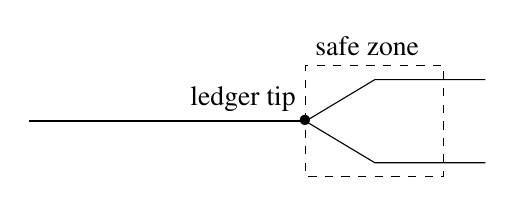
\begin{tikzpicture}[baseline=0pt]
\draw [thick] (-50pt,0) -- (50pt, 0) coordinate (tip);
\draw (tip) -- ++(25pt,  15pt) -- ++(40pt, 0pt);
\draw (tip) -- ++(25pt, -15pt) -- ++(40pt, 0pt);
\node at (tip) {$\bullet$};
\node at (tip) [above left] {ledger tip};
\draw [dashed] (tip)
            -- ++(0pt, 20pt) node[above right] {safe zone}
            -- ++(50pt, 0pt) -- ++(0pt, -40pt) -- ++(-50pt, 0pt) -- cycle;
\end{tikzpicture}
\end{equation}

\section{Ledger restrictions}
\label{time:ledgerrestrictions}

\subsection{Era transitions must be stable}

Monotonicity (\cref{time-conversion-monotone}) only talks about a chain's linear
history; since the consensus layer needs to deal with rollbacks (switching to
alternative chains) too, we will actually need a stronger property. Clearly,
time conversions cannot be invariant under switching to arbitrary chains; after
all, alternative chains might have era transitions in different places. The
consensus layer however does not \emph{support} switching to arbitrary
alternative chains; we have a maximum rollback (\cref{param:k}), and we never
switch to a shorter chain (\cref{chain-selection:overview},
\cref{never-shrink}). This means that we can model switching to an alternative
chain as $$\switch{n}{bs}{\sigma}$$ where $n \le k$ indicates how many blocks we
want to rollback, $\mathit{bs}$ is a list of new blocks we want to apply, and
$\mathtt{length} \; \mathit{bs} \ge n$.

\begin{property}[Time conversions stable under chain evolution]
\label{time-stable-under-evolution}
If \timeconv{\sigma}{t} is defined, then so is
\timeconv{\switch{n}{bs}{\sigma}}{t}
and moreover
\begin{equation*}
  \timeconv{\sigma}{t}
= \timeconv{\switch{n}{bs}{\sigma}}{t}
\end{equation*}
\end{property}

Intuitively, \cref{time-stable-under-evolution} says that we might not be able
to do time conversion for some time $t$ because it's outside our current forecast
range, but \emph{if} it is within forecast range, then we don't need to earmark
the answers we get from conversion as ``subject to rollback'': either we don't
know, or we know for sure. This requirement may not be strictly \emph{required}
for consensus to operate (\cref{future:relax-time-requirements}), but it is
a useful assumption which simplifies reasoning about time both within consensus
and within clients of the consensus layer such as the wallet.

The existence of safe zones is not sufficient to establish this stronger
property, in two ways:

\begin{itemize}
\item If we switch from a chain where an era transition is already known but
far in the future, to a chain on which the era transition happens much sooner
(or indeed, to a chain on which the era transition is not yet known), then
the forecast range will shrink and hence
\timeconv{\switch{n}{bs}{\sigma}}{t}
might not be defined, even if \timeconv{\sigma}{t} is.
\item Conversely, if we switch from a chain on which the era transition is
happening relatively soon, to a chain on which the era transition is happening
later, then the forecast range will not shrink, but the time conversions on
both chains will not agree with each other.\footnote{Going from a
chain on which the era transition is not yet known to one in which it \emph{is}
known is not problematic, due to safe zones.}
\end{itemize}

The key problem is that switching to an alternative chain can change our
information about future era transitions, and hence result in different time
conversions. We therefore insist that an era transition is not considered
``known'' until the block confirming the era transition is stable (no longer
subject to rollback). This means that the minimum distance from the announcement
of the era transition to the actual era transition must be $k$ plus the width of
the safe zone:
%
\begin{equation}
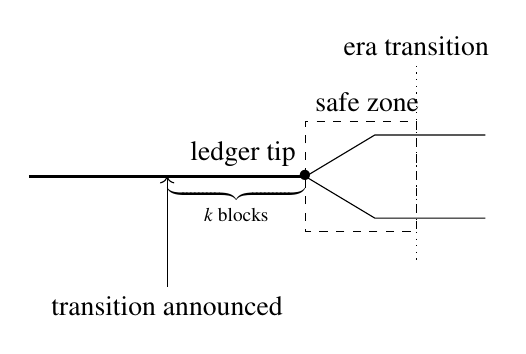
\begin{tikzpicture}[baseline=0pt]
\draw [thick] (-50pt,0) -- (50pt, 0) coordinate (tip);
\draw (tip) -- ++(25pt,  15pt) -- ++(40pt, 0pt);
\draw (tip) -- ++(25pt, -15pt) -- ++(40pt, 0pt);
\node at (tip) {$\bullet$};
\node at (tip) [above left] {ledger tip};
\draw [dashed] (tip)
            -- ++(0pt, 20pt) node[above right] {safe zone}
            -- ++(40pt, 0pt) coordinate (transition)
            -- ++(0pt, -40pt) -- ++(-40pt, 0pt) -- cycle;
\draw [dotted] (transition) ++(0pt, 20pt) node[above] {era transition}
            -- ++(0pt, -70pt);
\draw [<-] (tip) ++(-50pt, 0)
        -- +(0,-40pt) node[below] {transition announced};
% again, cheating...
\node at (25pt, -10pt) {$\underbrace{\hspace{50pt}}_\textrm{$k$ blocks}$};
\end{tikzpicture}
\end{equation}
%
Many ledgers set the width of the safe zone such that it guarantees at least $k$
blocks, but \emph{in principle} there is no need for the width of the safe zone
to be related to $k$ at all, although other parts of consensus might have
requirements for the width of the safe zone; we will discuss that in the next
section (\cref{time:ledgerrestrictions:safezones}).

\subsection{Size of the safezones}
\label{time:ledgerrestrictions:safezones}

The most important example of where we might need to do time translation for
blocks ahead of the ledger's tip is forecasting the Shelley ledger view
(\cref{ledger:forecasting}). The Shelley ledger view contains an abstraction
called \lstinline!EpochInfo! allowing the ledger to do time conversions, for
example to decide when rewards should be allocated.

As discussed in \cref{forecast:ledgerview}, it is important that the forecast
range of the ledger to allow us to validate at least $k + 1$ blocks after the
ledger tip; consequently, the safe zone of the ledger must be wide enough to
guarantee that it can span $k + 1$ blocks. This combination of the requirements
of the ledger with the header/body split
(\cref{nonfunctional:network:headerbody}) means that in practice the width of
the safe zone should be at least equal to the forecast range of the ledger, and
hence defined in terms of $k$ after all.

\subsection{Stability should not be approximated}

We discussed in \cref{time:slots-vs-blocks} that the ledger uses uses slot
numbers to approximate stability. Such an approximation would violate
\cref{time-stable-under-evolution}, however. Although we never switch to a
shorter chain in terms of blocks, it is certainly possible that we might switch
to a chain with a smaller \emph{slot} number at its tip: this would happen
whenever we switch to a longer but denser chain. If stability would be based on
slot numbers, this might mean that we could go from a situation in which the era
transition is considered known (and hence the forecast extends into the next
era) to a situation in which the era transition is not yet considered known (and
hence the forecast range only includes the safe zone in the current era).

Admittedly such a reduction of the forecast range would be temporary, and once
the era transition is considered known again, it will be in the same location;
after all, the block that confirmed the era transition \emph{is} stable. This
means that any previously executed time conversions would remain to be valid;
however, the fact that the forecast range shrinks might lead to unexpected
surprises. Using blocks rather than slot numbers to determine stability avoids
this problem.

\section{Properties}

\subsection{Forecast ranges arising from safe zones}

Slot length and epoch size can only change at era transitions. This means that
if the transition to the next era is not yet known, any time $t$ within the
era's safe zone is guaranteed to be within the era's forecast range. If the
transition to the next era \emph{is} known, the safe zone of the current era is
not relevant, but the safe zone of the next era is:
%
\begin{equation}
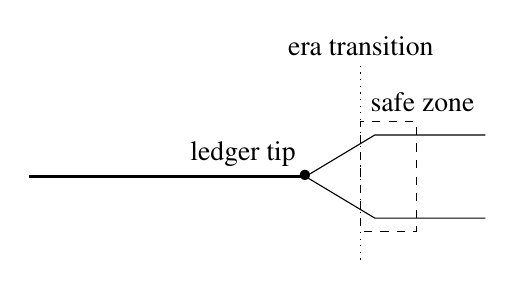
\begin{tikzpicture}[baseline=0pt]
\draw [thick] (-50pt,0) -- (50pt, 0) coordinate (tip);
\draw (tip) -- ++(25pt,  15pt) -- ++(40pt, 0pt);
\draw (tip) -- ++(25pt, -15pt) -- ++(40pt, 0pt);
\node at (tip) {$\bullet$};
\node at (tip) [above left] {ledger tip};
\draw [dashed] (tip) ++(20pt, 0pt) coordinate (transition)
            -- ++(0pt, 20pt) node[above right] {safe zone}
            -- ++(20pt, 0pt) -- ++(0pt, -40pt) -- ++(-20pt, 0pt) -- cycle;
\draw [dotted] (transition) ++(0pt, 40pt) node[above] {era transition}
            -- ++(0pt, -70pt);
\end{tikzpicture}
\end{equation}
%
The safe zone of the next era might be smaller or larger than (or indeed of
equal size as) the safe zone of the previous era; in this example it happens to
be smaller.

\Cref{hfc:era-transition-becoming-known} shows how the forecast range changes as
the next era transition becomes known; as shown, the next era starts at the
earliest possible moment (right after the safe zone); in general it could start
later than that, but of course not earlier (that would violate the definition of
the safe zone).

\begin{figure}

\begin{equation}
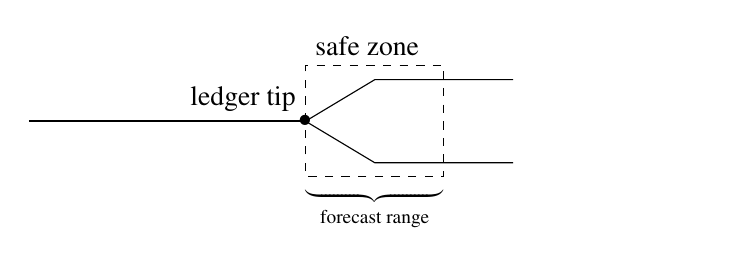
\begin{tikzpicture}[baseline=0pt]
\path (0,0) -- ++(200pt, 0pt); % adjust bounding box
\draw [thick] (-50pt,0) -- (50pt, 0) coordinate (tip);
\draw (tip) -- ++(25pt,  15pt) -- ++(50pt, 0pt);
\draw (tip) -- ++(25pt, -15pt) -- ++(50pt, 0pt);
\node at (tip) {$\bullet$};
\node at (tip) [above left] {ledger tip};
\draw [dashed] (tip)
            -- ++(0pt, 20pt) node[above right] {safe zone}
            -- ++(50pt, 0pt)
            -- ++(0pt, -40pt)
            -- ++(-50pt, 0pt) coordinate[pos=0.5] (safezone)
            -- cycle;
\node at (safezone) [below] {$\underbrace{\hspace{50pt}}_\textrm{forecast range}$};
\end{tikzpicture}
\end{equation}

\begin{equation}
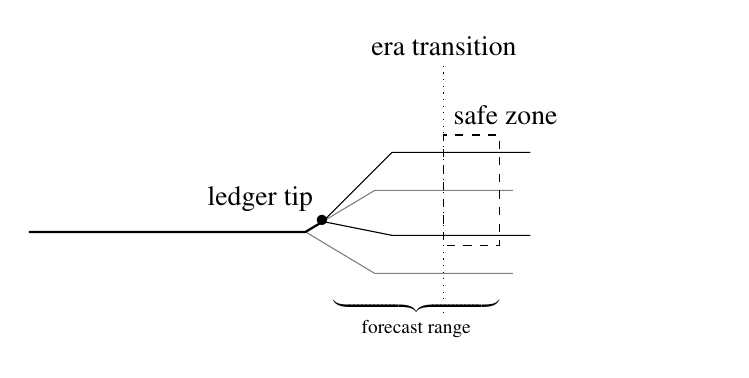
\begin{tikzpicture}[baseline=0pt]
\path (0,0) -- ++(200pt, 0pt); % adjust bounding box
\draw [gray] (-50pt,0) -- (50pt, 0) coordinate (oldtip);
\draw [gray, name path=chaintop] (oldtip) -- ++(25pt, 15pt) coordinate[pos=0.25] (tip) -- ++(50pt, 0pt);
\draw [gray] (oldtip) -- ++(25pt, -15pt) -- ++(50pt, 0pt);
\draw [thick] (-50pt,0) -- (50pt, 0) -- (tip);
\node at (tip) {$\bullet$};
\node at (tip) [above left] {ledger tip};
\draw (tip) -- ++(25pt, 25pt) -- +(50pt, 0pt);
\draw (tip) -- ++(25pt, -5pt) -- +(50pt, 0pt);
\draw [dotted, name path=transition]
        (oldtip) ++(50pt, 60pt) node[above] {era transition}
              -- ++(0pt, -90pt);
\path [name intersections={of=transition and chaintop}]
        (intersection-1) coordinate (safezone);
\draw [dashed] (safezone)
            -- ++(0pt, 20pt) node[above right] {safe zone}
            -- ++(20pt, 0pt)
            -- ++(0pt, -40pt)
            -- ++(-20pt, 0pt) coordinate[pos=0.5] (safezone)
            -- cycle;

% cheat: we should compute this of course :)
\node at (90pt,-20pt) [below] {$\underbrace{\hspace{60pt}}_\textrm{forecast range}$};
\end{tikzpicture}
\label{forecast-range-known-era-transition}
\end{equation}
\caption{\label{hfc:era-transition-becoming-known}Era transition becoming known}
\end{figure}

\subsection{Cross-fork conversions}
\label{time:cross-fork}

\begin{lemma}[Cross fork conversions]
Suppose we have the ledger state at some point $P$, and want to do time
conversions for time $t$ of a point $Q$ on a different fork of the chain:

\begin{center}
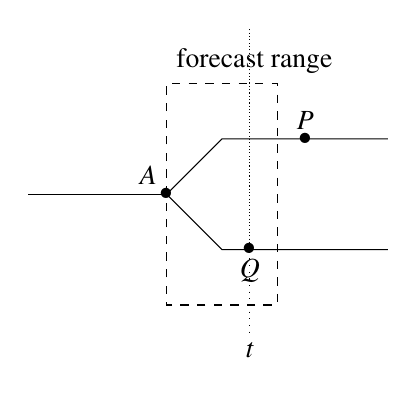
\begin{tikzpicture}
\draw (0,0) -- (50pt, 0) coordinate (A);
\draw (A) -- ++(20pt, 20pt)
          -- ++(30pt, 0) coordinate(P)
          -- ++(30pt, 0);
\draw (A) -- ++(20pt, -20pt)
          -- ++(10pt, 0) coordinate(Q1)
          -- ++(40pt, 0) coordinate(Q2)
          -- ++(10pt, 0);
\node at (A) {$\bullet$};
\node at (A) [above left] {$A$};
\node at (P) {$\bullet$};
\node at (P) [above] {$P$};
\node at (Q1) {$\bullet$};
\node at (Q1) [below] {$Q$};
\draw [dashed] (A) -- ++(0, 40pt) node[above right] {forecast range}
                   -- ++(40pt, 0)
                   -- ++(0, -80pt)
                   -- ++(-40pt, 0)
                   -- cycle;
\draw [dotted] (Q1) -- +(0, 80pt) -- +(0, -30pt) node[below] {$t$};
\end{tikzpicture}
\end{center}

Provided that $Q$ is within the forecast range of the common ancestor $A$
of $P$ and $Q$, the ledger state at $P$ can be used to do time conversions
for point $t$.
\end{lemma}

\begin{proof}
Since $t$ is within the forecast range at $A$, by definition $\timeconv{A}{t}$
is defined. By monotonicity (\cref{time-conversion-monotone}) we must have
\begin{align*}
\timeconv{A}{t} & = \timeconv{P}{t} \\
\timeconv{A}{t} & = \timeconv{Q}{t}
\end{align*}
It follows that $\timeconv{P}{t} = \timeconv{Q}{t}$.
\end{proof}

\section{Avoiding time}
\label{hfc:avoiding-time}

Time is complicated, and time conversions were pervasive throughout the
consensus layer. Despite the exposition above and the increased understanding,
we nonetheless have attempted to limit the use of time as much as possible,
in an attempt to simplify reasoning whenever possible. The use of
time within the core consensus layer is now very limited indeed:

\begin{enumerate}
\item When we check if we are a slot leader and need to produce a block, we
need to know the current time as a slot number (\todo{TODO.}We should discuss
this somewhere. The chapter on the consensus protocol discusses the protocol
side of things, but not the actual ``fork block production'' logic.)
\item When we add new blocks to the chain DB, we need to check if their slot
number is ahead of the wallclock (\cref{storage:infuture}).
\item Specific consensus protocols may need to do time conversions; for example,
Praos needs to know when various points in an epoch have been reached in order
to update nonces, switch stake distribution, etc.
\end{enumerate}

None of these use cases require either forecasting or cross-chain conversions.
The most important example of where forecasting is required is in projecting
the ledger view, as discussed in \cref{time:ledgerrestrictions:safezones}.
Cross-fork conversions (\cref{time:cross-fork}) may arise for example when the consensus layer makes time conversions available to tooling such as the wallet,
which may use it for example to show the wallclock of slots of blocks that may
not necessarily live on the current chain.

Keeping track of era transitions, and providing time conversions that take
them into account, is the responsibility of the hard fork combinator and
we will discuss it in more detail in \cref{hfc:time}.

In the remainder of this section we will discuss some simplifications
that reduced the reliance on time within the consensus layer.

\subsection{``Header in future'' check}
\label{time:header-infuture-check}

Recall from \cref{nonfunctional:network:headerbody} that block downloading
proceeds in two steps: first, the chain sync client downloads the block header
and validates it; if it finds that the header is valid, the block download logic
may decide to also download the block body, depending on chain selection
(\cref{chain-selection}).

Suppose the node's own ledger state is at point $P$, and the incoming header is
at point $Q$. In order to validate the header, we need a ledger \emph{view} at
point $Q$ without having the ledger \emph{state} at point $Q$; this means that
point $Q$ must be within the ledger's forecast range at the common ancestor $A$
of $P$ and $Q$ (\cref{class:ConsensusProtocol:ledgerview,ledger:forecasting}):

\begin{center}
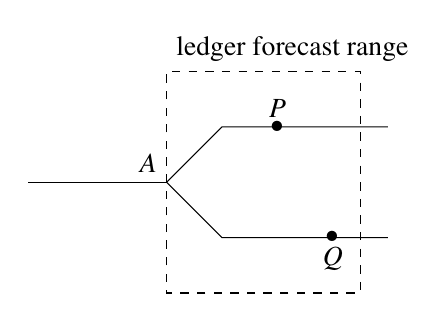
\begin{tikzpicture}
\draw (0, 0) -- (50pt, 0) coordinate (A);
\draw (A) -- ++(20pt,  20pt) -- ++(20pt, 0) coordinate (P) -- ++(40pt, 0);
\draw (A) -- ++(20pt, -20pt) -- ++(40pt, 0) coordinate (Q) -- ++(20pt, 0);
\node at (P) {$\bullet$};
\node at (Q) {$\bullet$};
\node at (A) [above left] {$A$};
\node at (P) [above] {$P$};
\node at (Q) [below] {$Q$};
\draw [dashed] (A) -- ++(0, 40pt) node[above right] {ledger forecast range}
                   -- ++(70pt, 0)
                   -- ++(0, -80pt)
                   -- ++(-70pt, 0)
                   -- cycle;
\end{tikzpicture}
\end{center}

As we have seen in \cref{time:cross-fork}, if $Q$ is within the \emph{time}
forecast range at $A$---put another way, if the time forecast range is at least
as wide as the ledger forecast range---then we also can use the ledger state at
$P$ to do time conversions at point $Q$. Moreover, as we saw in
\cref{time:ledgerrestrictions:safezones}, for many ledgers that inclusion
\emph{must} hold. If we make this a requirement for \emph{all} ledgers, in
principle the chain sync client could do a header-in-future check.

For simplicity, however, we nonetheless omit the check. As we will see in the
next section, the chain database must repeat this check \emph{anyway}, and so
doing it ahead of time in the chain sync client does not help very much;
skipping it avoids one more use of time within the consensus layer. Indeed, a
case could be made that we could skip header validation altogether, which would
alleviate the need for forecasting \emph{at all}; we will come back to this in
\cref{future:eliminating-forecasting}.

\subsection{Ahead-of-time ``block in future'' check}
\label{time:block-infuture-check}

In the original design of the chain database, when a new block was added we
first checked if the block's slot number was ahead of the wallclock, before
considering it for chain selection. If it was ahead of the wallclock by a small
amount (within the permissible clock skew), we then scheduled an action to
reconsider the block when its slot arrived.

In order to compare the block's slot number to the wallclock, we can either
convert the block's slot to a wallclock time, or convert the current wallclock
time to a slot number. Both are problematic: the only ledger state we have
available is our own current ledger state, which may not be usable to translate
the current wallclock time to a slot number, and since we don't know anything
about the provenance of the block (where the block came from), that ledger state
may also not be usable to translate the block's slot number to a wallclock
time. We now circumvent this problem by delaying the in-future check until we
have validated the block, and so can use the block's \emph{own} ledger state to
do the time conversion (\cref{storage:infuture}).

We saw in the previous section that the chain sync client \emph{could} do the
in-future check on headers, but the chain sync client is not the only way that
blocks can be added to the chain database, so simply skipping the check in the
chain database altogether, stipulating as a \emph{precondition} that the block
is not ahead of the wallclock, is not a good idea. Nonetheless it is worth
considering if we could use a weaker precondition, merely requiring that the
node's current ledger tip must be usable for time conversions for the slot
number of the new block. Specifically, can we guarantee that we can satisfy this
precondition in the chain sync client, if we do the in-future check on headers
after all?

It turns out that in general we cannot, not even in relatively common cases.
Consider again the diagram from \cref{time:header-infuture-check}, but
specialised to the typical case that the upstream node is on the same chain as
we are, but a bit ahead of us:

\begin{center}
\begin{tikzpicture}
\path (0,0) -- ++(200pt, 0pt); % adjust bounding box
\draw (0, 0) -- (50pt, 0) coordinate (A) coordinate (P);
\draw (A) -- ++(20pt, 0pt) -- ++(20pt, 0) -- ++(40pt, 0);
\draw (A) -- ++(20pt, 0pt) -- ++(40pt, 0) coordinate (Q) -- ++(20pt, 0);
\node at (P) {$\bullet$};
\node at (Q) {$\bullet$};
\node at (A) [above left] {$A$};
\node at (A) {$\bullet$};
\node at (P) [below left] {$P$};
\node at (Q) [below] {$Q$};
\draw [dashed] (A) -- ++(0, 20pt) node[above right] {forecast range}
                   -- ++(70pt, 0)
                   -- ++(0, -40pt)
                   -- ++(-70pt, 0)
                   -- cycle;
\end{tikzpicture}
\end{center}

Since $P$ and $Q$ are on the same chain,  point $P$ is necessarily also the
``intersection'' point, and the distance between $P$ and $Q$ can only arise from
the block download logic lagging behind the chain sync client.
Now consider what happens when the node switches to an alternative fork:

\begin{center}
\begin{tikzpicture}
\path (0,0) -- ++(200pt, 0pt); % adjust bounding box
\draw (0, 0) -- (30pt, 0) coordinate (A);
\draw (A) -- ++(20pt,  20pt) -- ++(20pt, 0) coordinate (P) -- ++(60pt, 0);
\draw (A) -- ++(20pt, -20pt) -- ++(60pt, 0) coordinate (Q) -- ++(20pt, 0);
\node at (P) {$\bullet$};
\node at (Q) {$\bullet$};
\node at (A) [above left] {$A$};
\node at (P) [above] {$P$};
\node at (Q) [below] {$Q$};
\draw [dashed] (A) -- ++(0, 40pt) node[above right] {forecast range}
                   -- ++(70pt, 0)
                   -- ++(0, -80pt)
                   -- ++(-70pt, 0)
                   -- cycle;
\end{tikzpicture}
\end{center}

Note what happens: since the node is switching to another fork, it must rollback
some blocks and then roll forward; consequently, the intersection point $A$
moves back, and $P$ moves forward (albeit on a different chain). $Q$ stays the
same, \emph{but might have fallen out of the forecast range at $A$}.

This means that even if the chain sync client was able to verify that a header
(at point $Q$) was not ahead of the wallclock, if the node switches to a
different fork before the block download logic has downloaded the corresponding
block, when it presents that downloaded block to the chain database, the block
might no longer be within the forecast range of the node's current ledger and
the chain database will not be able to verify (ahead of time) whether or not the
block is ahead of the wallclock. What's worse, unlike the chain sync client, the
chain database has no access to the intersection point $A$; it all it has is the
ledger's current tip at  point $P$ and the new block at point $Q$. It therefore
has no reliable way of even determining \emph{if} it can do time conversions for
the new block.

\subsection{``Immutable tip in future'' check}
\label{time:imm-tip-in-future}

The chain database never adopts blocks from the future
(\cref{storage:infuture}). Nevertheless, it is possible that if the user sets
their computer system clock back by (the equivalent of) more than $k$ blocks,
the immutable database (\cref{storage:components}) might contain blocks
whose slot numbers are ahead of the wall clock. We cannot verify this during a
regular integrity check of the immutable database because, as we have seen in
this chapter, we would need a ledger state to do so, which we are not
constructing during that integrity check. For now, we simply omit this check
altogether, declaring it to be the user's responsibility instead to do a
fresh install if they do reset their clock by this much.

However, in principle this check is not difficult: we initialise the immutable
DB \emph{without} doing the check, then initialise the ledger DB, passing it the
immutable DB (which it needs to replay the most recent blocks, see
\cref{ledgerdb}), and then ask the ledger DB for the ledger state
corresponding to the tip of the immutable database. That ledger state will then
allow us to do time conversions for any of the blocks in the immutable DB,
trimming any blocks that are ahead of the wallclock.

\subsection{Scheduling actions for slot changes}
\label{time:scheduling-actions}

The consensus layer provides an abstraction called \lstinline!BlockchainTime!
that provides access to the current slot number. It also offers an interface
for scheduling actions to be run on every slot change. However, if the node
is still syncing with the chain, and does not have a recent ledger state
available, the current slot number, and indeed the current slot length,
are simply unknown. In this case the blockchain time will report the current
slot number as unavailable, and any scheduled actions will not be run.

We therefore limit the use of this scheduler to a single application only:
it is used to trigger the leadership check (and corresponding block
production, if we find we are a leader). This means that the leadership
check will not be run if we are still syncing with the chain and have no
recent ledger state available, but that is correct: producing blocks based on
ancient ledger states is anyway not useful.

\subsection{Switching on ``deadline mode'' in the network layer}

Under normal circumstances, the priority of the network layer is to reduce
\emph{latency}: when a block is produced, it must be distributed across the
network as soon as possible, so that the next slot leader can construct the
\emph{next} block as this block's successor; if the block arrives too late,
the next slot leader will construct their block as the successor of the previous
block instead, and the chain temporarily forks.

When we are far behind, however, the priority is not to reduce latency, but
rather to improve \emph{throughput}: we want to catch up as quickly as we can
with the chain, and aren't producing blocks anyway
(\cref{time:scheduling-actions}).

In order to switch between these two modes we want to know if we are near the
tip of the ledger---but how can we tell? If we know the current slot number
(the slot number corresponding to the current wall clock), we can compare
that current slot number to the slot number at the tip of the ledger. But,
as we mentioned before, if we are far behind, the current slot number of
simply unknown. Fortunately, we can use this to our advantage: if the
slot number is unknown, we \emph{must} be far behind, and hence we can use
the decision, turning on deadline mode only if the slot number is known
\emph{and} within a certain distance from the ledger tip.

\chapter{Miscellaneous}

TODO\todo{TODO}: This is a mess at the moment.

\section{On abstraction}

ledger integration: as things were changing a lot, it made sense for consensus to define the ledger API internally and have the integration be done consensus side. but as things are stabilising, it might make more sense for that abstraction to live externally, so that you can literally plug in Shelley into consensus and we don't have to do anything

\section{On-disk ledger state}

\duncan

Sketch out what we think it could look like
Consequences for the design

\section{Transaction TTL}
\label{future:ttl}

Describe that the mempool could have explicit support for TTL, but that right now we don't (and why this is OK: the ledger anyway checks tx TTL). We should discuss why this is not an attack vector (transactions will either be included in the blockchain or else will be chucked out because some of their inputs will have been used).

\section{Block based versus slot based}
\label{future:block-vs-slot}

\section{Eliminating safe zones}
\label{future:eliminating-safezones}

Are they really needed? Consensus doesn't really look ahead anymore?
(Headers are not checked for time; leadership is ticking, not forecasting).
Does the wallet really need it? What about the ledger?

Other thought: what if we split slots into "microslots", 20 microslots to a
slot. Now the slot/time mapping is \emph{always} known, and for Shelley etc
we don't actually need to know the global microslot, all we care about is
the microslot within a slot (and hence is independent of when Shelley starts).
This would make time conversion no longer state dependent.

\section{Eliminating forecasting}
\label{future:eliminating-forecasting}

This is a stronger version of \cref{future:eliminating-safezones}, where
we eliminate \emph{all} forecasting. Specifically, this means that we don't
do header validation anymore, relying on the chain DB to do block validation.
This would be an important simplification of the consensus layer, but we'd
need to analyse what the ``benefit'' of this simplification is for an
attacker. Personally, I think it'll be okay.

The most important analysis we need to do here is how this affects the memory
usage of the chain sync client. Note that we already skip the ahead-of-time
check, which we don't do until we have the full block and validate it. We
should discuss that somewhere as well.

\section{Open kinds}
\label{future:openkinds}

Avoid type errors such as trying to apply a ledger to a block instead of an era
(or an era instead of crypto, or..).

\section{Relax requirements on time conversions}
\label{future:relax-time-requirements}

Perhaps it would be okay if time conversions we strictly relative to a ledger
state, rather than ``absolute'' (\cref{time:ledgerrestrictions}).

\section{Configuration}

What a mess.

\section{Specialised chain selection data structure}

In \cref{chainsel:spec} we describe how chain selection is implemented. However,
in an ideal world this would mean we have some kind of specialised data
structure supporting

\begin{itemize}
\item Efficient insertion of new blocks
\item Efficient computation of the best chain
\end{itemize}

It's however not at all clear what such a data structure would look like if we
don't want to hard-code the specific chain selection rule.

\section{Dealing with clock changes}
\label{future:clockchanges}

When the user changes their system clock, blocks that we previously adopted
into our current chain might now be ahead of the system clock (\cref{chainsel:infuture}) and should not
be part of the chain anymore, and vice versa.

When the system clock of a node is moved \emph{forward}, we should run chain
selection again because some blocks that we stored because they were in the
future may now become valid. Since this could be any number of blocks, on any
fork, probably easiest to just do a full chain selection cycle (starting from
the tip of the immutable database).

When the clock is moved \emph{backwards}, we may have accepted blocks that we
should not have. Put another way, an attacker might have taken advantage of the
fact that the clock was wrong to get the node to accept blocks in the future. In
this case we therefore really should rollback--- but this is a weird kind of
rollback, one that might result in a strictly smaller current chain. We can only
do this by re-initialising the chain DB from scratch (the ledger DB does not
support such rollback directly). Worse still, we have have decided that some
blocks were immutable which really weren't.

Unlike the data corruption case, here we should really endeavour to get to a
state in which it was as if the clock was never ``wrong'' in the first place;
this may mean we might have to move some blocks back from the immutable DB to
the volatile DB, depending on exactly how far the clock was moved back and how
big the overlap between the immutable DB and volatile DB is.

It is therefore good to keep in mind that the overlap between the immutable DB
and volatile DB does make it a bit easier to deal with relatively small clock
changes; it may be worth ensuring that, say, the overlap is at least a few days
so that we can deal with people turning back their clock a day or two without
having to truncate the immutable database. Indeed, in a first implementation,
this may be the \emph{only} thing we support, though we will eventually have to
lift that restriction.

Right now, we do nothing special when the clock moves forward (we will discover
discover the now valid blocks on the next call to \lstinline!addBlock!
(\cref{chainsel:addblock}). When the clock is reset \emph{backwards}, the node
will currently (intentionally) crash, we make no attempt to try and reset
the state (the current slot number moving backwards might cause difficulties
in many places). Unfortunately, if the clock is moved so far back that blocks
in the \emph{immutable database} are now considered to be ahead of the wall
clock, we will not currently detect this (\cref{time:imm-tip-in-future}).


\part{Testing}

\chapter{Reaching consensus}
\label{testing:consensus}

\section{Dire-but-not-to-dire}
\label{testing:dire}

We should mention the PBFT threshold here \cref{bft-paper}.

\chapter{The storage layer}
\label{testing:storage}


\part{Conclusions}

\chapter{Technical design decisions}
\label{technical}

In this chapter we will discuss a number of interesting technical decision
decisions that aren't directly to any of the specific needs of the consensus
layer.

\section{Classes versus records}
\label{technical:classes-vs-records}

Discuss why classes are helpful (explicit about closures).

\section{Top-level versus associated type families}
\label{technical:toplevel-vs-associated}

\chapter{Future work}

\section{On abstraction}

ledger integration: as things were changing a lot, it made sense for consensus to define the ledger API internally and have the integration be done consensus side. but as things are stabilising, it might make more sense for that abstraction to live externally, so that you can literally plug in Shelley into consensus and we don't have to do anything

\section{Genesis}
\label{future:genesis}

Genesis is problematic for at least two reasons:

\begin{itemize}
\item It does not fit the look-at-tip-only approach we use
\item It violates the ``we never roll back to a shorter chain'' assumption.
\end{itemize}

\section{On-disk ledger state}

\duncan

Sketch out what we think it could look like
Consequences for the design

\section{Transaction TTL}
\label{future:ttl}

Describe that the mempool could have explicit support for TTL, but that right now we don't (and why this is OK: the ledger anyway checks tx TTL). We should discuss why this is not an attack vector (transactions will either be included in the blockchain or else will be chucked out because some of their inputs will have been used).

\section{Block based versus slot based}
\label{future:block-vs-slot}

\section{Eliminating safe zones}
\label{future:eliminating-safezones}

Are they really needed? Consensus doesn't really look ahead anymore?
(Headers are not checked for time; leadership is ticking, not forecasting).
Does the wallet really need it? What about the ledger?

Other thought: what if we split slots into "microslots", 20 microslots to a
slot. Now the slot/time mapping is \emph{always} known, and for Shelley etc
we don't actually need to know the global microslot, all we care about is
the microslot within a slot (and hence is independent of when Shelley starts).
This would make time conversion no longer state dependent.

\section{Eliminating forecasting}
\label{future:eliminating-forecasting}

This is a stronger version of \cref{future:eliminating-safezones}, where
we eliminate \emph{all} forecasting. Specifically, this means that we don't
do header validation anymore, relying on the chain DB to do block validation.
This would be an important simplification of the consensus layer, but we'd
need to analyse what the ``benefit'' of this simplification is for an
attacker. Personally, I think it'll be okay.

The most important analysis we need to do here is how this affects the memory
usage of the chain sync client. Note that we already skip the ahead-of-time
check, which we don't do until we have the full block and validate it. We
should discuss that somewhere as well.

\section{Open kinds}
\label{future:openkinds}

Avoid type errors such as trying to apply a ledger to a block instead of an era
(or an era instead of crypto, or..).

\section{Relax requirements on time conversions}
\label{future:relax-time-requirements}

Perhaps it would be okay if time conversions we strictly relative to a ledger
state, rather than ``absolute'' (\cref{time:ledgerrestrictions}).

\section{Configuration}

What a mess.

\section{Specialised chain selection data structure}

In \cref{chainsel:spec} we describe how chain selection is implemented. However,
in an ideal world this would mean we have some kind of specialised data
structure supporting

\begin{itemize}
\item Efficient insertion of new blocks
\item Efficient computation of the best chain
\end{itemize}

It's however not at all clear what such a data structure would look like if we
don't want to hard-code the specific chain selection rule.

\section{Dealing with clock changes}
\label{future:clockchanges}

When the user changes their system clock, blocks that we previously adopted
into our current chain might now be ahead of the system clock (\cref{chainsel:infuture}) and should not
be part of the chain anymore, and vice versa.

When the system clock of a node is moved \emph{forward}, we should run chain
selection again because some blocks that we stored because they were in the
future may now become valid. Since this could be any number of blocks, on any
fork, probably easiest to just do a full chain selection cycle (starting from
the tip of the immutable database).

When the clock is moved \emph{backwards}, we may have accepted blocks that we
should not have. Put another way, an attacker might have taken advantage of the
fact that the clock was wrong to get the node to accept blocks in the future. In
this case we therefore really should rollback--- but this is a weird kind of
rollback, one that might result in a strictly smaller current chain. We can only
do this by re-initialising the chain DB from scratch (the ledger DB does not
support such rollback directly). Worse still, we have have decided that some
blocks were immutable which really weren't.

Unlike the data corruption case, here we should really endeavour to get to a
state in which it was as if the clock was never ``wrong'' in the first place;
this may mean we might have to move some blocks back from the immutable DB to
the volatile DB, depending on exactly how far the clock was moved back and how
big the overlap between the immutable DB and volatile DB is.

It is therefore good to keep in mind that the overlap between the immutable DB
and volatile DB does make it a bit easier to deal with relatively small clock
changes; it may be worth ensuring that, say, the overlap is at least a few days
so that we can deal with people turning back their clock a day or two without
having to truncate the immutable database. Indeed, in a first implementation,
this may be the \emph{only} thing we support, though we will eventually have to
lift that restriction.

Right now, we do nothing special when the clock moves forward (we will discover
discover the now valid blocks on the next call to \lstinline!addBlock!
(\cref{chainsel:addblock}). When the clock is reset \emph{backwards}, the node
will currently (intentionally) crash, we make no attempt to try and reset
the state (the current slot number moving backwards might cause difficulties
in many places). Unfortunately, if the clock is moved so far back that blocks
in the \emph{immutable database} are now considered to be ahead of the wall
clock, we will not currently detect this (\cref{time:imm-tip-in-future}).

\chapter{Conclusions}


\part{Appendices}
\appendix

\chapter{Byron}

Some details specific to the Byron ledger.
EBBs already discussed at length in \cref{ebbs}.

The Byron specification can be found at \url{https://github.com/input-output-hk/cardano-ledger-specs}.

\section{Update proposals}
\label{byron:hardfork}

\subsection{Moment of hard fork}
\label{byron:hardfork:moment}

The Byron ledger state provides the current protocol version in
%
\begin{lstlisting}
adoptedProtocolVersion :: ProtocolVersion
\end{lstlisting}
%
in the \lstinline!State! type from
\lstinline!Cardano.Chain.Update.Validation.Interface!.
This protocol version is a three-tuple \emph{major}, \emph{minor}, \emph{alt}.
The Byron specification does not provide any semantic interpretation of these
components. By convention (outside of the purview of the Byron specification),
the hard fork is initiated the moment that the \emph{major} component of
\lstinline!adoptedProtocolVersion! reaches a predefined, hardcoded, value.

\subsection{The update mechanism for the \lstinline!ProtocolVersion!}

Updates to the \lstinline!ProtocolVersion! in Byron are part of the general
infrastructure for changing protocol parameters (parameters such as the maximum
block size), except that in the case of a hard fork, we care only about changing
the \lstinline!ProtocolVersion!, and not any of the parameters themselves.

The general mechanism for updating protocol parameters in Byron is as follows:

\begin{enumerate}

\item
A protocol update \emph{proposal} transaction is created. It proposes new values
for some protocol parameters and a greater \emph{protocol version} number as an
identifier. There cannot be two proposals with the same version number.

\item
Genesis key delegates can add \emph{vote} transactions that refer to such a
proposal (by its hash). They don't have to wait; a node could add a proposal and
a vote for it to its mempool simultaneously. There are only positive votes, and
a proposal has a time-to-live (see \lstinline!ppUpdateProposalTTL!) during which
to gather sufficient votes. While gathering votes, a proposal is called
\emph{active}.

Note that neither Byron nor Shelley support full centralisation (everybody can
vote); this is what the Voltaire ledger is intended to accomplish.

\item
Once the number of voters satisfies a threshold (currently determined by the
\lstinline!srMinThd! field of the \lstinline!ppSoftforkRule! protocol
parameter), the proposal becomes \emph{confirmed}.

\item
Once the threshold-satisfying vote becomes stable (i.e. its containing block is at
least $2k$ slots deep), a block whose header's protocol version number
(\lstinline!CC.Block.headerProtocolVersion!) is that of the proposal is
interpreted as an \emph{endorsement} of the stably-confirmed proposal by the
block's issuer (specifically by the Verification Key of its delegation
certificate). Endorsements---i.e. \emph{any block}, since they all contain that
header field---also trigger the system to discard proposals that were not
confirmed within their TTL.

Notably, endorsements for proposals that are not yet stably-confirmed (or do not
even exist) are not invalid but rather silently ignored. In other words, no
validation applies to the `headerProtocolVersion` field.

\item
Once the number of endorsers satisfies a threshold (same as for voting), the
confirmed proposal becomes a \emph{candidate} proposal.

\item
\emph{At the beginning of an epoch}, the candidate proposal with the greatest
protocol version number among those candidates whose threshold-satisfying
endorsement is stable (i.e. the block is at least $2k$ deep) is \emph{adopted}:
the new protocol parameter values have now been changed.

If there was no stable candidate proposal, then nothing happens. Everything is
retained; in particular, a candidate proposal whose threshold-satisfying
endorsement was not yet stable will be adopted at the subsequent epoch unless it
is surpassed in the meantime.

When a candidate is adopted, all record of other
proposals/votes/endorsements---regardless of their state---is discarded. The
explanation for this is that such proposals would now be interpreted as an
update to the newly adopted parameter values, whereas they were validated as an
update to the previously adopted parameter values.

\end{enumerate}

The diagram shown in \cref{byron:update-process} summarises the progress of a
proposal that's eventually adopted. For other proposals, the path short circuits
to a ``rejected/discarded'' status at some point.

\begin{figure}
\hrule
\begin{center}
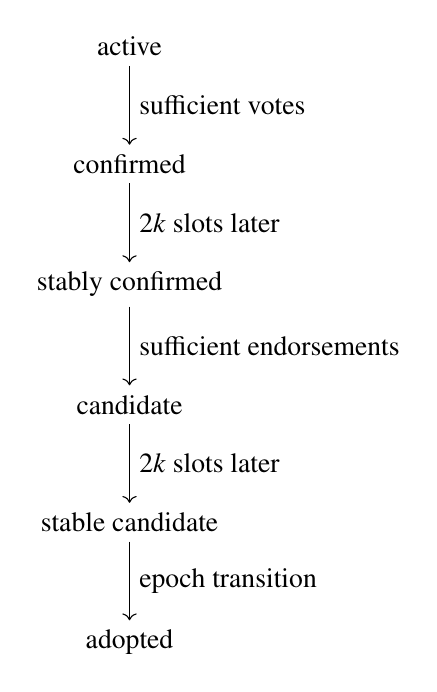
\begin{tikzpicture}
\node (act)                {active}           ;
\node (con) [below=of act] {confirmed}        ;
\node (sta) [below=of con] {stably confirmed} ;
\node (can) [below=of sta] {candidate}        ;
\node (sca) [below=of can] {stable candidate} ;
\node (ado) [below=of sca] {adopted}          ;
\draw[->] (act.south) -- (con.north) node[pos=0.5, right] {sufficient votes};
\draw[->] (con.south) -- (sta.north) node[pos=0.5, right] {$2k$ slots later};
\draw[->] (sta.south) -- (can.north) node[pos=0.5, right] {sufficient endorsements};
\draw[->] (can.south) -- (sca.north) node[pos=0.5, right] {$2k$ slots later};
\draw[->] (sca.south) -- (ado.north) node[pos=0.5, right] {epoch transition};
\end{tikzpicture}
\end{center}
\hrule
\caption{\label{byron:update-process}Byron update proposal process}
\end{figure}

\subsection{Initiating the hard fork}
\label{byron:hardfork:initiating}

Proposals to initiate the hard fork can be submitted and voted on before all
core nodes are ready. After all, once a proposal is stably confirmed, it will
effectively remain so indefinitely until nodes endorse it (or it gets superseded
by another proposal). This means that nodes can vote to initiate the hard fork,
\emph{then} wait for everybody to update their software, and once updated, the
proposal is endorsed and eventually the hard fork is initiated.

Endorsement is somewhat implicit. The node operator does not submit an explicit
``endorsement transaction'', but instead restarts the
node\footnote{\label{byron:unnecessary-restarts}A node restart is necessary for
\emph{any} change to a protocol parameter, even though most parameters do not
require any change to the software at all.} (probably after a software update
that makes the node ready to support the hard fork) with a new protocol version
(as part of a configuration file or command line parameter), which then gets included
in the blocks that the node produces (this value is the
\lstinline!byronProtocolVersion! field in the static \lstinline!ByronConfig!).

\subsection{Software versions}

The Byron ledger additionally also records the latest version of the software on
the chain, in order to facilitate software discovering new versions and
subsequently updating themselves. This would normally precede all of the above,
but as far as the consensus layer is concerned, this is entirely orthogonal. It
does not in any way interact with either the decision to hard fork nor the
moment of the hard fork. If we did forego it, the discussion above would still
be entirely correct. As of Shelley, software discovery is done off-chain.

The Byron \emph{block header} also records a software version
(\lstinline!headerSoftwareVersion!). This is a legacy concern only, and is
present in but ignored by the current Byron implementation, and entirely absent
from the Byron specification.

\chapter{Shelley}

\section{Update proposals}
\label{shelley:hardfork}

\subsection{Moment of the hard fork}
\label{shelley:hardfork:moment}

Similar to the Byron ledger (\cref{byron:hardfork:moment}), the Shelley ledger
provides a ``current protocol version'', but it is a two-tuple (not a
three-tuple), containing only a \emph{hard fork} component and \emph{soft fork}
component:
%
\begin{lstlisting}
_protocolVersion :: (Natural, Natural)
\end{lstlisting}
%
in \lstinline!PParams!. The hard fork from Shelley to its successor will be
initiated once the hard fork component of this version gets incremented.

\subsection{The update mechanism for the protocol version}

The update mechanism in Shelley is simpler than it is in Byron. There is no
distinction between votes and proposals: to ``vote'' for a proposal one merely
submits the exact same proposal. There is also no separate endorsement step
(though see \cref{shelley:hardfork:initiating}).

The procedure is as follows:

\begin{enumerate}

\item
As in Byron, a proposal is a partial map from parameters to their values.

\item
During each epoch, a genesis key can submit (via its delegates) zero, one, or
many proposals; each submission overrides the previous one.

\item
``Voting'' (submitting of proposals) ends $6k/f$ slots before the end of the
epoch (i.e., twice the stability period, called \lstinline!stabilityWindow! in
the Shelley ledger implementation).

\item
At the end of an epoch, if the majority of nodes (as determined by the
\lstinline!Quorum! specification constant, which must be greater than half the
nodes) have most recently submitted the same exact proposal, then it is adopted.

\item
The next epoch is always started with a clean slate, proposals from the
previous epoch that didn't make it are discarded.\footnote{Proposals \emph{can}
be explicitly marked to be for future epochs; in that case, these are simply
not considered until that epoch is reached.}

\end{enumerate}

The protocol version itself is also considered to be merely another parameter,
and parameters can change without changing the protocol version, although a
convention could be established that the protocol version must change if any of
the parameters do; but the specification itself does not mandate this.

\subsection{Initiating the hard fork}
\label{shelley:hardfork:initiating}

The timing of the hard fork in Shelley is different to the one in Byron: in
Byron, we \emph{first} vote and then wait for people to get ready
(\cref{byron:hardfork:initiating}); in Shelley it is the other way around.

Core node operators will want to know that a significant majority of the core
nodes is ready (supports the hard fork) before initiating it. To make this
visible, Shelley blocks contain a protocol version. This is not related to the
current protocol version as reported by the ledger state
(\lstinline!_protocolVersion! as discussed in the previous section), but it is
the \emph{maximum} protocol version that the node which produced that block can
support.

Once we see blocks from all or nearly all core nodes with the `hard fork`
component of their protocol version equal to the post-hard-fork value, nodes
will submit their proposals with the required major version change to initiate
the hard fork.\footnote{This also means that unlike in Byron
(\cref{byron:unnecessary-restarts}), in Shelley there is no need to restart the
node merely to support a particular parameter change (such as a maximum block
size).}

\section{Forecasting}
\label{shelley:forecasting}

Discuss the fact that the effective maximum rollback in Shelley is $k - 1$,
not $k$; see also \cref{ledger:forecasting}.


\bibliographystyle{acm}
\bibliography{references}

\end{document}
